%File: formatting-instructions-latex-2024.tex
%release 2024.0
\documentclass[letterpaper]{article} % DO NOT CHANGE THIS
\usepackage{aaai24}  % DO NOT CHANGE THIS
\usepackage{times}  % DO NOT CHANGE THIS
\usepackage{helvet}  % DO NOT CHANGE THIS
\usepackage{courier}  % DO NOT CHANGE THIS
\usepackage[hyphens]{url}  % DO NOT CHANGE THIS
\usepackage{graphicx} % DO NOT CHANGE THIS
\urlstyle{rm} % DO NOT CHANGE THIS
\def\UrlFont{\rm}  % DO NOT CHANGE THIS
\usepackage{natbib}  % DO NOT CHANGE THIS AND DO NOT ADD ANY OPTIONS TO IT
\usepackage{caption} % DO NOT CHANGE THIS AND DO NOT ADD ANY OPTIONS TO IT
\frenchspacing  % DO NOT CHANGE THIS
\setlength{\pdfpagewidth}{8.5in}  % DO NOT CHANGE THIS
\setlength{\pdfpageheight}{11in}  % DO NOT CHANGE THIS
%
% These are recommended to typeset algorithms but not required. See the subsubsection on algorithms. Remove them if you don't have algorithms in your paper.
\usepackage{algorithm}
\usepackage{algorithmic}

\usepackage{graphicx}
\usepackage{multirow}
\usepackage{relsize}


%
% These are are recommended to typeset listings but not required. See the subsubsection on listing. Remove this block if you don't have listings in your paper.
\usepackage{newfloat}
\usepackage{listings}
\DeclareCaptionStyle{ruled}{labelfont=normalfont,labelsep=colon,strut=off} % DO NOT CHANGE THIS
\lstset{%
	basicstyle={\footnotesize\ttfamily},% footnotesize acceptable for monospace
	numbers=left,numberstyle=\footnotesize,xleftmargin=2em,% show line numbers, remove this entire line if you don't want the numbers.
	aboveskip=0pt,belowskip=0pt,%
	showstringspaces=false,tabsize=2,breaklines=true}
\floatstyle{ruled}
\newfloat{listing}{tb}{lst}{}
\floatname{listing}{Listing}
%
% Keep the \pdfinfo as shown here. There's no need
% for you to add the /Title and /Author tags.
\pdfinfo{
/TemplateVersion (2024.1)
}

% DISALLOWED PACKAGES
% \usepackage{authblk} -- This package is specifically forbidden
% \usepackage{balance} -- This package is specifically forbidden
% \usepackage{color (if used in text)
% \usepackage{CJK} -- This package is specifically forbidden
% \usepackage{float} -- This package is specifically forbidden
% \usepackage{flushend} -- This package is specifically forbidden
% \usepackage{fontenc} -- This package is specifically forbidden
% \usepackage{fullpage} -- This package is specifically forbidden
% \usepackage{geometry} -- This package is specifically forbidden
% \usepackage{grffile} -- This package is specifically forbidden
% \usepackage{hyperref} -- This package is specifically forbidden
% \usepackage{navigator} -- This package is specifically forbidden
% (or any other package that embeds links such as navigator or hyperref)
% \indentfirst} -- This package is specifically forbidden
% \layout} -- This package is specifically forbidden
% \multicol} -- This package is specifically forbidden
% \nameref} -- This package is specifically forbidden
% \usepackage{savetrees} -- This package is specifically forbidden
% \usepackage{setspace} -- This package is specifically forbidden
% \usepackage{stfloats} -- This package is specifically forbidden
% \usepackage{tabu} -- This package is specifically forbidden
% \usepackage{titlesec} -- This package is specifically forbidden
% \usepackage{tocbibind} -- This package is specifically forbidden
% \usepackage{ulem} -- This package is specifically forbidden
% \usepackage{wrapfig} -- This package is specifically forbidden
% DISALLOWED COMMANDS
% \nocopyright -- Your paper will not be published if you use this command
% \addtolength -- This command may not be used
% \balance -- This command may not be used
% \baselinestretch -- Your paper will not be published if you use this command
% \clearpage -- No page breaks of any kind may be used for the final version of your paper
% \columnsep -- This command may not be used
% \newpage -- No page breaks of any kind may be used for the final version of your paper
% \pagebreak -- No page breaks of any kind may be used for the final version of your paperr
% \pagestyle -- This command may not be used
% \tiny -- This is not an acceptable font size.
% \vspace{- -- No negative value may be used in proximity of a caption, figure, table, section, subsection, subsubsection, or reference
% \vskip{- -- No negative value may be used to alter spacing above or below a caption, figure, table, section, subsection, subsubsection, or reference

\setcounter{secnumdepth}{0} %May be changed to 1 or 2 if section numbers are desired.

% The file aaai24.sty is the style file for AAAI Press
% proceedings, working notes, and technical reports.
%

% Title

% Your title must be in mixed case, not sentence case.
% That means all verbs (including short verbs like be, is, using,and go),
% nouns, adverbs, adjectives should be capitalized, including both words in hyphenated terms, while
% articles, conjunctions, and prepositions are lower case unless they
% directly follow a colon or long dash
\title{Auto311: A Confidence-guided Automated System for Non-emergency Call}
\author {
    % Authors
    Zirong Chen\textsuperscript{\rm 1},
    Xutong Sun\textsuperscript{\rm 1},
    Yuanhe Li\textsuperscript{\rm 1},
    Meiyi Ma\textsuperscript{\rm 1}
}
\affiliations {
    % Affiliations
    \textsuperscript{\rm 1}Department of Computer Science, Vanderbilt University, Nashville, Tennessee 37235, USA\\
    \{zirong.chen, xutong.sun, yuanhe.li, meiyi.ma\}@vanderbilt.edu
}

%Example, Single Author, ->> remove \iffalse,\fi and place them surrounding AAAI title to use it
\iffalse
\title{My Publication Title --- Single Author}
\author {
    Author Name
}
\affiliations{
    Affiliation\\
    Affiliation Line 2\\
    name@example.com
}
\fi


%Example, Multiple Authors, ->> remove \iffalse,\fi and place them surrounding AAAI title to use it



% REMOVE THIS: bibentry
% This is only needed to show inline citations in the guidelines document. You should not need it and can safely delete it.
\usepackage{bibentry}
% END REMOVE bibentry

\begin{document}

\maketitle

\begin{abstract}
% Effective responses to emergencies and non-emergencies are essential for disaster management and can help reduce potential life-threatening consequences. However, dispatching centers often do not have the resources to handle all calls, regardless of when or where they occur. In this study, we analyzed audio recordings from the Nashville Metropolitan Government Dispatching Center, developed an assistant system to help the dispatchers quickly and accurately classify non-emergency calls and highlight important context information from the ongoing call to help the dispatchers quickly and easily file a report. We also evaluated our system under real-world conditions to assess its effectiveness. From the experimental results, we find our system can accurately give out classification results with an average F-1 score of 92.54\%. With the help of the confidence-aware features in key information identification, our system is tested to successfully highlight the most essential context to file a report with an average consistency score of 0.9329 when compared to the ground truth. From our emulated results, our system helps reduce the conversation by 1.01 turns on average only based on the context information in the first few rounds and also offers call dispatching suggestions with an average accuracy of 94.49\%.

% Emergency and non-emergency services perform as critical gateways between residents and first responders. Effective emergency and non-emergency response proves essential for disaster management. However, despite responders' and governments' best efforts, the sheer volume of 911 emergency and 311 non-emergency calls combined with severe labor shortages have heavily burdened existing infrastructure in the USA. 
Emergency and non-emergency response systems are essential services provided by local governments and critical to
protecting lives, the environment, and property. The effective handling of (non-)emergency calls is critical for public safety and well-being. 
% Emergency and non-emergency services play a vital role as connections between residents and first responders. 
% It is crucial to have efficient responses for both situations to manage disasters effectively. 
By reducing the
burden through non-emergency callers, residents in critical need of assistance through 911 will receive fast
and effective response. 
Collaborating with the Department of Emergency Communications (DEC) in Nashville, we analyzed 11,796 non-emergency call recordings and developed Auto311\footnote{Code and Demo: https://github.com/AICPS-Lab/Auto311}, the first
automated system to handle 311 non-emergency calls, which (1) effectively and dynamically predicts ongoing non-emergency incident types to generate tailored case reports during the call; (2) itemizes essential information from dialogue contexts to complete the generated reports; and (3) strategically structures system-caller dialogues with optimized confidence. We used real-world data to evaluate the system's effectiveness and deployability. The experimental results indicate that the system effectively predicts incident type with an average F-1 score of 92.54\%. Moreover, the system successfully itemizes critical information from relevant contexts to complete reports, evincing a 0.93 average consistency score compared to the ground truth. Additionally, emulations demonstrate that the system effectively decreases conversation turns as the utterance size gets more extensive and categorizes the ongoing call with 94.49\% mean accuracy. 

% Emergency and non-emergency services act as critical gateways between residents and first responders. Effective responses to emergencies and non-emergencies prove essential for disaster management. However, despite the best efforts by responders and governments, the sheer volume of emergency (911) and non-emergency (311) calls, coupled with a severe labor shortage, have put immense strain on the existing infrastructure in the USA. This study analyzes audio recordings from the Nashville Metropolitan Government Dispatch Center. We develop an automated system to (1) accurately and dynamically predict the ongoing incident type(s) of non-emergency calls to generate specific case reports, (2) itemize essential information to complete the generated case report, (3) and strategically organize the dialogue between our system and the caller with optimized system confidence scores. Furthermore, this study evaluates the system using real-world data to assess effectiveness and potential adaptability. The experimental results indicate the system can provide accurate classification with an average F-1 score of 92.54\%. By implementing confidence-aware features in key information identification, the system successfully itemizes essential information from the most vital context to complete the reports with an average consistency score of 0.9329 compared to the ground truth. Additionally, emulated results demonstrate that the system decreases conversation turns by 1.01 on average solely based on early contextual information while offering call dispatch suggestions with 94.49\% average accuracy.

% highlight salient contextual information from ongoing calls to expedite dispatcher report filing. 

% dispatch centers across cities frequently lack sufficient resources to handle all calls irrespective of timing or location. 

% Emergency and non-emergency services act as critical gateways between residents and first responders. Despite the best efforts by responders and governments, the sheer volume of emergency 


% (2) developed a tool to help dispatchers quickly and accurately identify the key information from callers, and (3) evaluated the tool under real-world conditions to assess its effectiveness, adaptability, and robustness.
\end{abstract}
\section{Introduction}
\label{sec:introduction}
\begin{figure}[t]
    \centering
    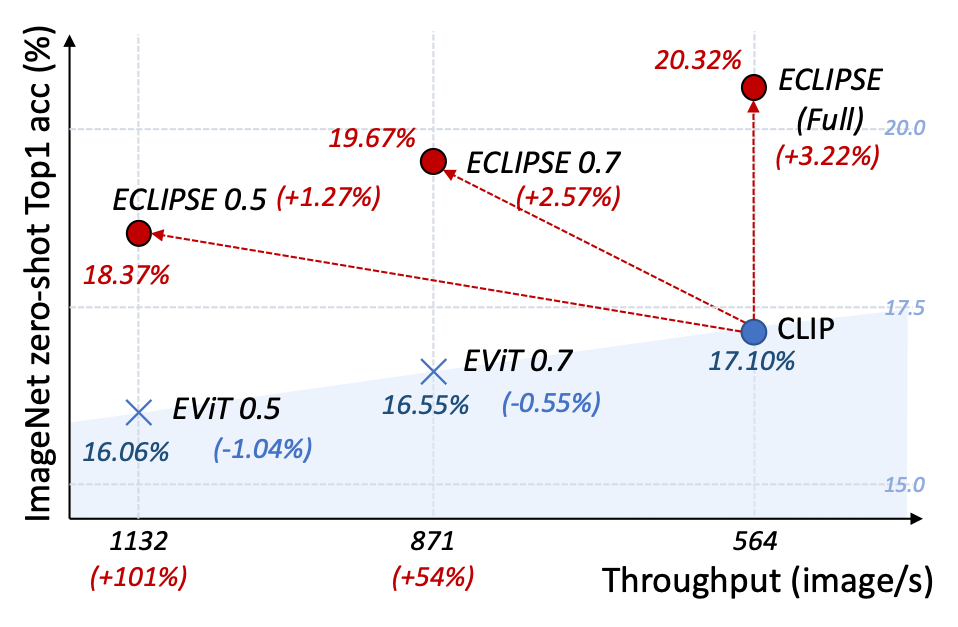
\includegraphics[width=0.9\columnwidth]{figures/imgs/figure_speed.png}
    \caption{Time vs. ImageNet zero-shot performance analysis for Contrastive Language-Image Pretraining with existing ViT accleration framework (EViT).
    We compare the results between EViT directly applied on CLIP and EViT trained with our proposed meta-architecture, ECLIPSE.
    Our proposed framework enables even streamlined ViTs with 101\% faster throughputs to outperform the full ViT of CLIP.
    Model performance and inference time are measured with ViT-B/16 backbone.
    }
    \label{fig:fig_speed}
\end{figure}
% Transformers in Computer vision
Transformers~\cite{vaswani2017attention} have achieved significant progress across various challenging vision tasks such as image classification~\cite{dosovitskiy2021an,touvron2021training,jiang2021all,graham2021levit}, object detection~\cite{carion2020end}, semantic segmentation~\cite{xie2021segformer,liu2021swin,wang2021pyramid} and visual relationship detection~\cite{kim2021hotr,kim2022mstr}.
% ViTs in Contrastive Language-Image Pretraining
Following this success in vision tasks, recent studies demonstrated that large-scale vision-language pretraining (VLP)~\cite{li2019visualbert,chen2019uniter,huang2019unicoder,li2020oscar,li2020unimo,lu2019vilbert,tan2019lxmert,jia2021scaling,radford2021learning} with ViTs is scalable to large uncurated datasets and transferable to various downstream tasks.

% Computational overhead of distillation
However, the large scale image-text pairs for VLP are usually collected from the web; thus they are often noisy, i.e., having weak correlation between the image and its corresponding text description.
To alleviate the image-text misalignment problem, previous works~\cite{li2021align,Lu2022COTS} have proposed knowledge distillation framework~\cite{hinton2015distilling} with a momentum encoder for both image and text.
However, adopting two additional momentum encoders and calculating soft alignments for distillation loss inevitably increase the computational cost for training, which hinders training for large-scale VLP.

% Efficient Distillation
In this work, we propose a efficient formulation for distilling soft image-text alignment matrix without text momentum encoder for contrastive language-image pretraining~\cite{jia2021scaling,radford2021learning}.
Inspired from SimSiam~\cite{chen2021exploring}, we simply replace the text momentum encoder with stop-gradient operation.
This design not only eliminates the computational cost for an additional text momentum encoder, but also enables the distillation to operate within a unified projected space of text embedding, resulting in better performance.
Based on this shared projected space, we adopt token sparsification~\cite{liang2022evit} for the online image encoder to i) provide a partial view that complementarily interacts with the full-view of the momentum image encoder, ii) compensate for the computational overhead of training the momentum image encoder, and iii) accelerate inference speed.
% Moreover, we further mitigate the heavy computational overhead by adopting token sparsification frameworks~\cite{liang2022evit} to expedite vision transformers which was originally proposed for supervised learning.
% Model acceleration can also improve inference speed unlike training acceleration via random masking of input patches~\cite{li2022scaling}.
% This unique design not only effectively improves data efficiency by alleviating the natural misalignment between images and text, but it also enhances computational efficiency by expediting online network.
While our distillation architecture effectively improves data efficiency by alleviating the natural misalignment between images and text, the expedited online image encoder and the momentum teacher positively interacts with a sweet spot that achieves speed improvement without degrading performance.
We name this meta-architecture as ECLIPSE: \textbf{E}xpediting \textbf{C}ontrastive \textbf{L}anguage-\textbf{I}mage \textbf{P}retraining with \textbf{S}elf-distilled \textbf{E}ncoders.
ECLIPSE is trained with a loss jointly obtained from two image-text alignment matrices (i.e., $\bar{A}$ and $A$ in Fig.~\ref{fig:fig_overview}):
\begin{itemize}
    \item The batch-wise image-text alignment matrix $\bar{A}$ between the text encoder and the momentum teacher is trained with an InfoNCE loss~\cite{oord2018representation} with hard alignment labels for matching image-text pairs.
    
    \item Student-text alignment matrix $A$ is obtained likewise with the online network and the text encoder with stop gradient. We train the online network to match $A$ with the soft alignment matrix $\bar{A}$ obtained above.
\end{itemize}
The momentum parameters are updated with an exponential moving average (EMA) of the parameters of online encoder.

Extensive experiments demonstrate the effectiveness of ECLIPSE, showing that our distillation architecture significantly improves data efficiency while achieving substantial model acceleration.
For example, when applied to CLIP~\cite{radford2021learning}, our proposed architecture improves 1.27\% zero-shot accuracy in ImageNet classification while achieving 101\% acceleration in inference speed.
Moreover, ECLIPSE can be also trained without expedition, which then shows a large 3.22\% gain compared to ViT, thus offers a model choice between an accelerated model with competitive performance and a full-capacity model with enhanced performance (see Fig.~\ref{fig:fig_speed} and Tab.~\ref{tab:keep}).
Furthermore, scaling to large-scale datasets, ECLIPSE achieves state-of-the-art on several downstream tasks, outperforming CLIP variants with a model accelerated by more than 54\%.

\begin{figure}
    \centering
    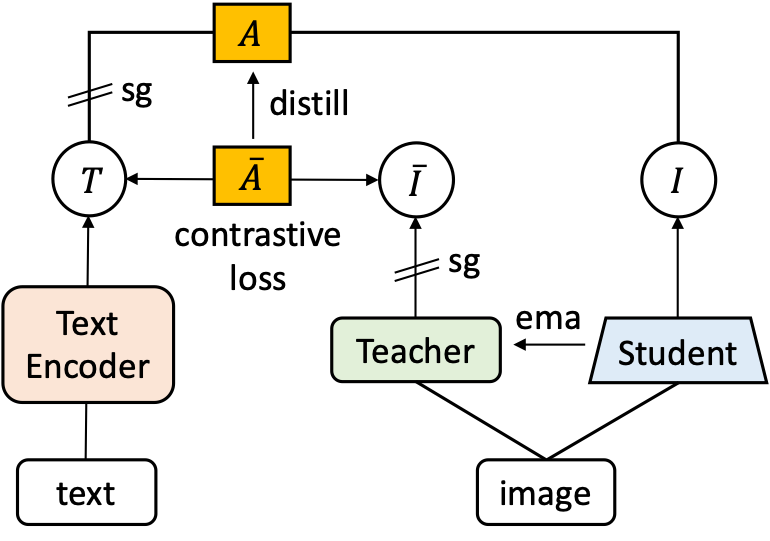
\includegraphics[width=0.8\columnwidth]{figures/imgs/figure_overview.png}
    \vspace{0.7em}
    \caption{Overview of ECLIPSE. Student encoder is trained to estimate the soft alignment matrix $\bar{A}$ predicted by Text Encoder and the Teacher network.
    sg stands for stop-gradient, $I$ and $\bar{I}$ are encoded image with student and teacher network, respectively.
    }
    \label{fig:fig_overview}
\end{figure}
\section{Motivating Study} 

% \subsection{Potential Urgent Situations \label{sec:motivation}} 
% Making seemingly routine calls to the local call center can conceal potentially urgent situations in various instances. Analysis of a large collection of audio transcriptions, conducted collaboratively with the call center team, reveals approximately 2,746 out of 4,640 transcriptions indicate possible urgent circumstances during the call. This finding highlights the urgency of developing an intelligible, manageable handover control system to promptly notify dispatchers when current calls imply urgent scenarios.


\subsubsection{Unintentional Additional Information}

 Examination of audio transcriptions indicates callers tend to provide supplementary details beyond the dispatcher's specific inquiries (72\% of callers offer extra information, exceeding the question's scope). Notably, this additional information can enhance the precision and comprehensiveness of the emergency response system. See the example below with the caller's personal information removed: 

$\mathsf{Dispatcher}$: Metro Nashville Police, Fire, and Medical, what is the location of your emergency? $\mathsf{Caller}$: Oh, I'm not sure if this is an emergency. I am \textit{\#name}, \textit{\#phone\_number}. The address is \textit{\#address}. It's the King Buffet. I got about a customer out in the parking lot smoking crackpipes in front of all the customers. 


% Here, despite the dispatcher asking about location, the caller additionallshares name, phone number, and suspicious activity details, hinting at a drug-related incident. Utilizing this information strategically could enhance emergency response talks, addressing follow-up queries preemptively, and streamlining interactions.

In this conversation turn, although the dispatcher only inquires about location, the caller provides additional details like name, phone number, and suspicious activity, suggesting a drug-related case. Strategically leveraging such extra information could optimize emergency response conversations by proactively addressing potential follow-up questions, thus streamlining the interaction. 

% Notably, only high-confidence answers undergo integration into the final report, achieved through an interactive confidence-checking process. This ensures maintained accuracy and reliability while restricting the final report to only the most relevant information.

\subsubsection{Shifting and Multiple Incident Types}
Call recordings show that ongoing incidents mentioned by callers occasionally encompass multiple incident types (at a rate of 38.27\%). Callers also tend to modify incident types as they uncover more details. For instance, phrases like ``someone busted my car and my wallet is gone'' indicate two incident types – damaged and lost stolen property. Similarly, in ``I saw a car illegally parked... oh, wait, it's abandoned because the bumper is off and rusted,'' the caller initially reports illegal parking, then recognizes it as an abandoned vehicle based on new details. This underscores the need for our system to recognize various incident types concurrently and adapt to evolving conversations.


% Based on the call recordings, the ongoing incident happening on the caller's side sometimes refers to multiple incident types (with a percentage of 38.27\%). Meanwhile, the caller might also tend to change the incident type with more details discovered. For example, ``...someone busted my car and my wallet is gone...'' indicates two incident types – ``someone busted my car'' suggests damage to property while ``my wallet is gone'' implies lost or stolen property. Also, in ``... I saw a car illegally parked at the same spot in the garage for a while... oh, wait I think it is abandoned instead cuz the bumper is off and rusted ...'', the caller was to report an illegal parking case, but then figured out this should be reported as an abandoned vehicle based on details like ``the bumper is off and rusted.'' This discovery necessitates that our system possesses the capability to simultaneously identify various types of incidents while also being adaptable to changes in the types of incidents as the conversation evolves.
\section{Overview of Auto311}

Auto311 is developed to autonomously handle non-emergency calls by engaging in interactive conversations with callers. An outline of our system's structure is shown in Figure \ref{fig:sys_overview}. The system comprises five key components: the \textit{conversational interface} for interacting with callers, the \textit{handover control} to transfer calls to human operators if needed, the \textit{incident type prediction} module to identify probable incident types, the \textit{information itemization} module to organize details in case reports, and the \textit{confidence-guided report generation and dialogue optimization} module for generating informed reports and optimizing subsequent conversations using confidence guidance.

% Auto311 has been designed to autonomously manage non-emergency calls, engaging in interactive conversations with non-emergency callers. An overview of our system's architecture is presented in Figure \ref{fig:sys_overview}. The system consists of five integral components: the \textit{conversational interface}, which facilitates interaction with callers; the \textit{handover control} function, responsible for directing calls to human operators when urgent situations arise; the \textit{incident type prediction} module, which identifies the most probable incident type(s) associated with the ongoing call; the \textit{information itemization} module, responsible for categorizing information into appropriate sections within the case report; and the \textit{confidence-guided report generation and dialogue optimization} module, ensuring the generation of a well-informed report and the optimization of subsequent dialogues with obtained confidence guidance.


% Auto311 is designed to handle non-emergency calls automatically. It interacts with the non-emergency callers in back-and-forth conversations. An overview of our system is shown in Figure \ref{fig:sys_overview}. There are five components of our system, including a \textit{conversational interface} to interact with the caller, a \textit{handover control} function to reroute calls to real operators in case of urgencies, an \textit{incident type prediction} module to indicate the most likely incident type(s) of the ongoing call, an \textit{information itemization} module to itemize the information based on the blank fields in the case report, and a \textit{confidence-guided report optimization} to ensure the report is generated. Future dialogue is optimized with obtained module outputs and corresponding confidence scores.

\begin{figure}[h]
    \centering
    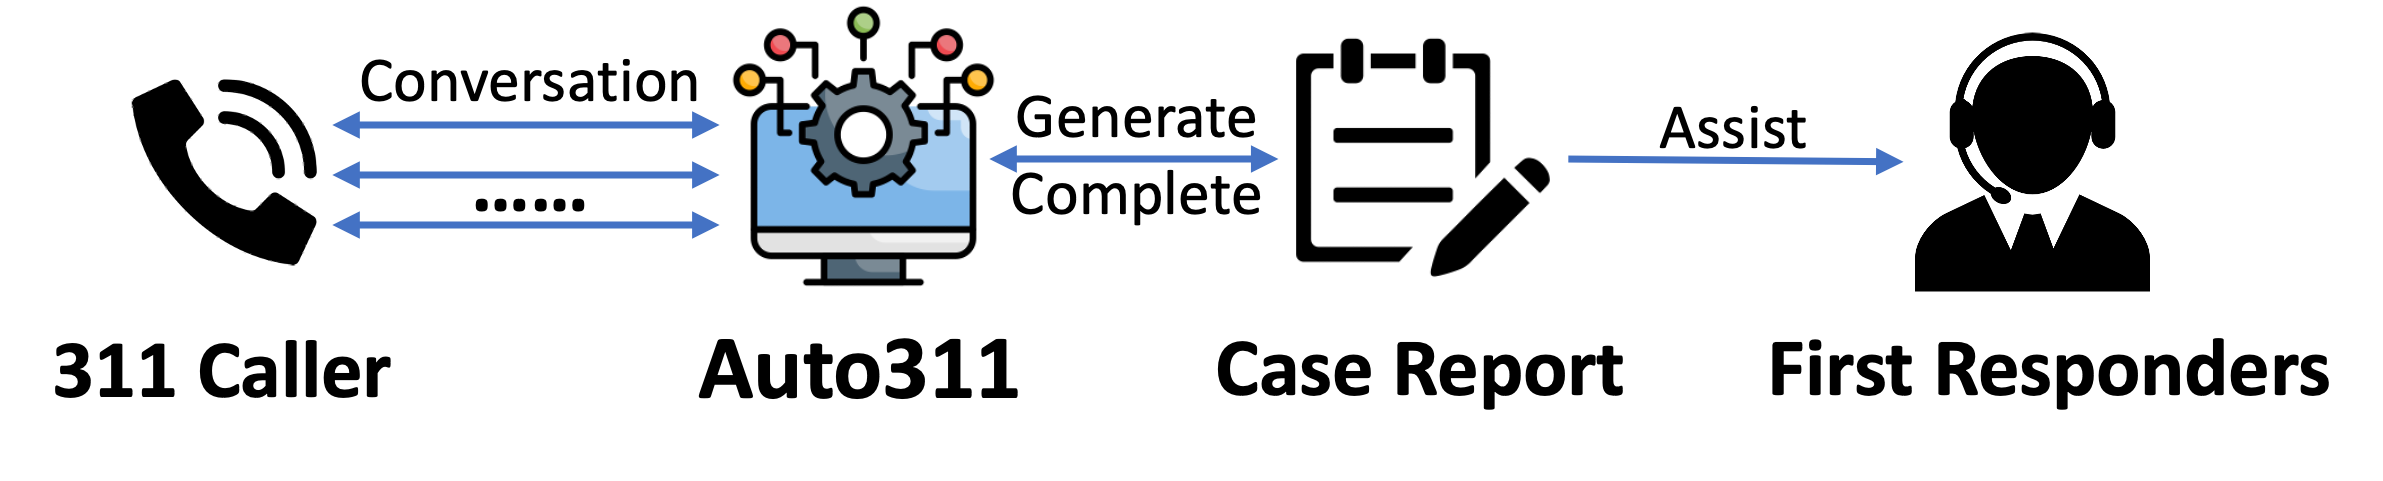
\includegraphics[width=0.4\textwidth]{figures/system_overview.png}
    \caption{Auto311 in Emergency Response}
    \label{fig:sys_overview}
    \vspace{-0.5cm}
\end{figure}

During runtime, as shown in Figure \ref{fig:sys_logic}, when a caller initiates contact, the \textit{conversational interface} starts the dialogue with opening questions, collecting essential information like the caller's name and incident location. Each response from the caller forms an utterance. Subsequently, the \textit{handover control} function evaluates whether human operator intervention is required for the call. The call proceeds to subsequent modules only if the handover is not needed. At the same time, the \textit{incident type prediction} module forecasts the most likely incident type(s) for report generation, while the \textit{information itemization} module provides potential details from the caller's utterance to fill the report's sections. Additionally, the \textit{confidence-guided report generation and dialogue optimization} module constantly monitors confidence scores to ensure the report is filled with high confidence, thereby optimizing follow-up conversations.

% During runtime, as illustrated in Figure \ref{fig:sys_logic}, when a caller initiates contact, the \textit{conversational interface} commences the dialogue by presenting opening questions, gathering fundamental information such as the caller's name and incident location. With each turn, the caller's response is captured as an utterance. Once the utterance is obtained, the \textit{handover control} function assesses whether a human operator's intervention is necessary for the ongoing call. Only if the handover control function's criteria are met does the call progress to subsequent modules. Concurrently, the \textit{incident type prediction} module anticipates the most probable incident type(s) to facilitate report generation, while the \textit{information itemization} module supplies potential details from the caller's utterance to complete the report's blank sections. Moreover, the \textit{confidence-guided report generation and dialogue optimization} module continuously monitors confidence scores to ensure that the report is enriched with maximum confidence, thereby optimizing follow-up dialogues.

% At runtime, shown in Figure \ref{fig:sys_logic}, upon a caller dials in, the \textit{conversational interface} initializes the dialogue with opening questions, querying basic questions, such as the caller's name and the location of the incident. At every turn, the caller's response is collected as an utterance. After obtaining the utterance, the \textit{handover control} function decides if a human operator needs to interfere with the current call. Only when the call clears the concerns of the handover control function, will it be passed to the subsequent modules. Meanwhile, the \textit{incident type prediction} module predicts the most likely incident type(s) to guide the report creation, and the \textit{information itemization} module offers potential information from caller utterance to the blank fields in the report. The \textit{confidence-guided report generation and dialogue optimization} module further tracks the confidence scores to make sure the report is updated with the maximized confidence so that the follow-up dialogues are optimized. 

\begin{figure*}[t]
    \centering
    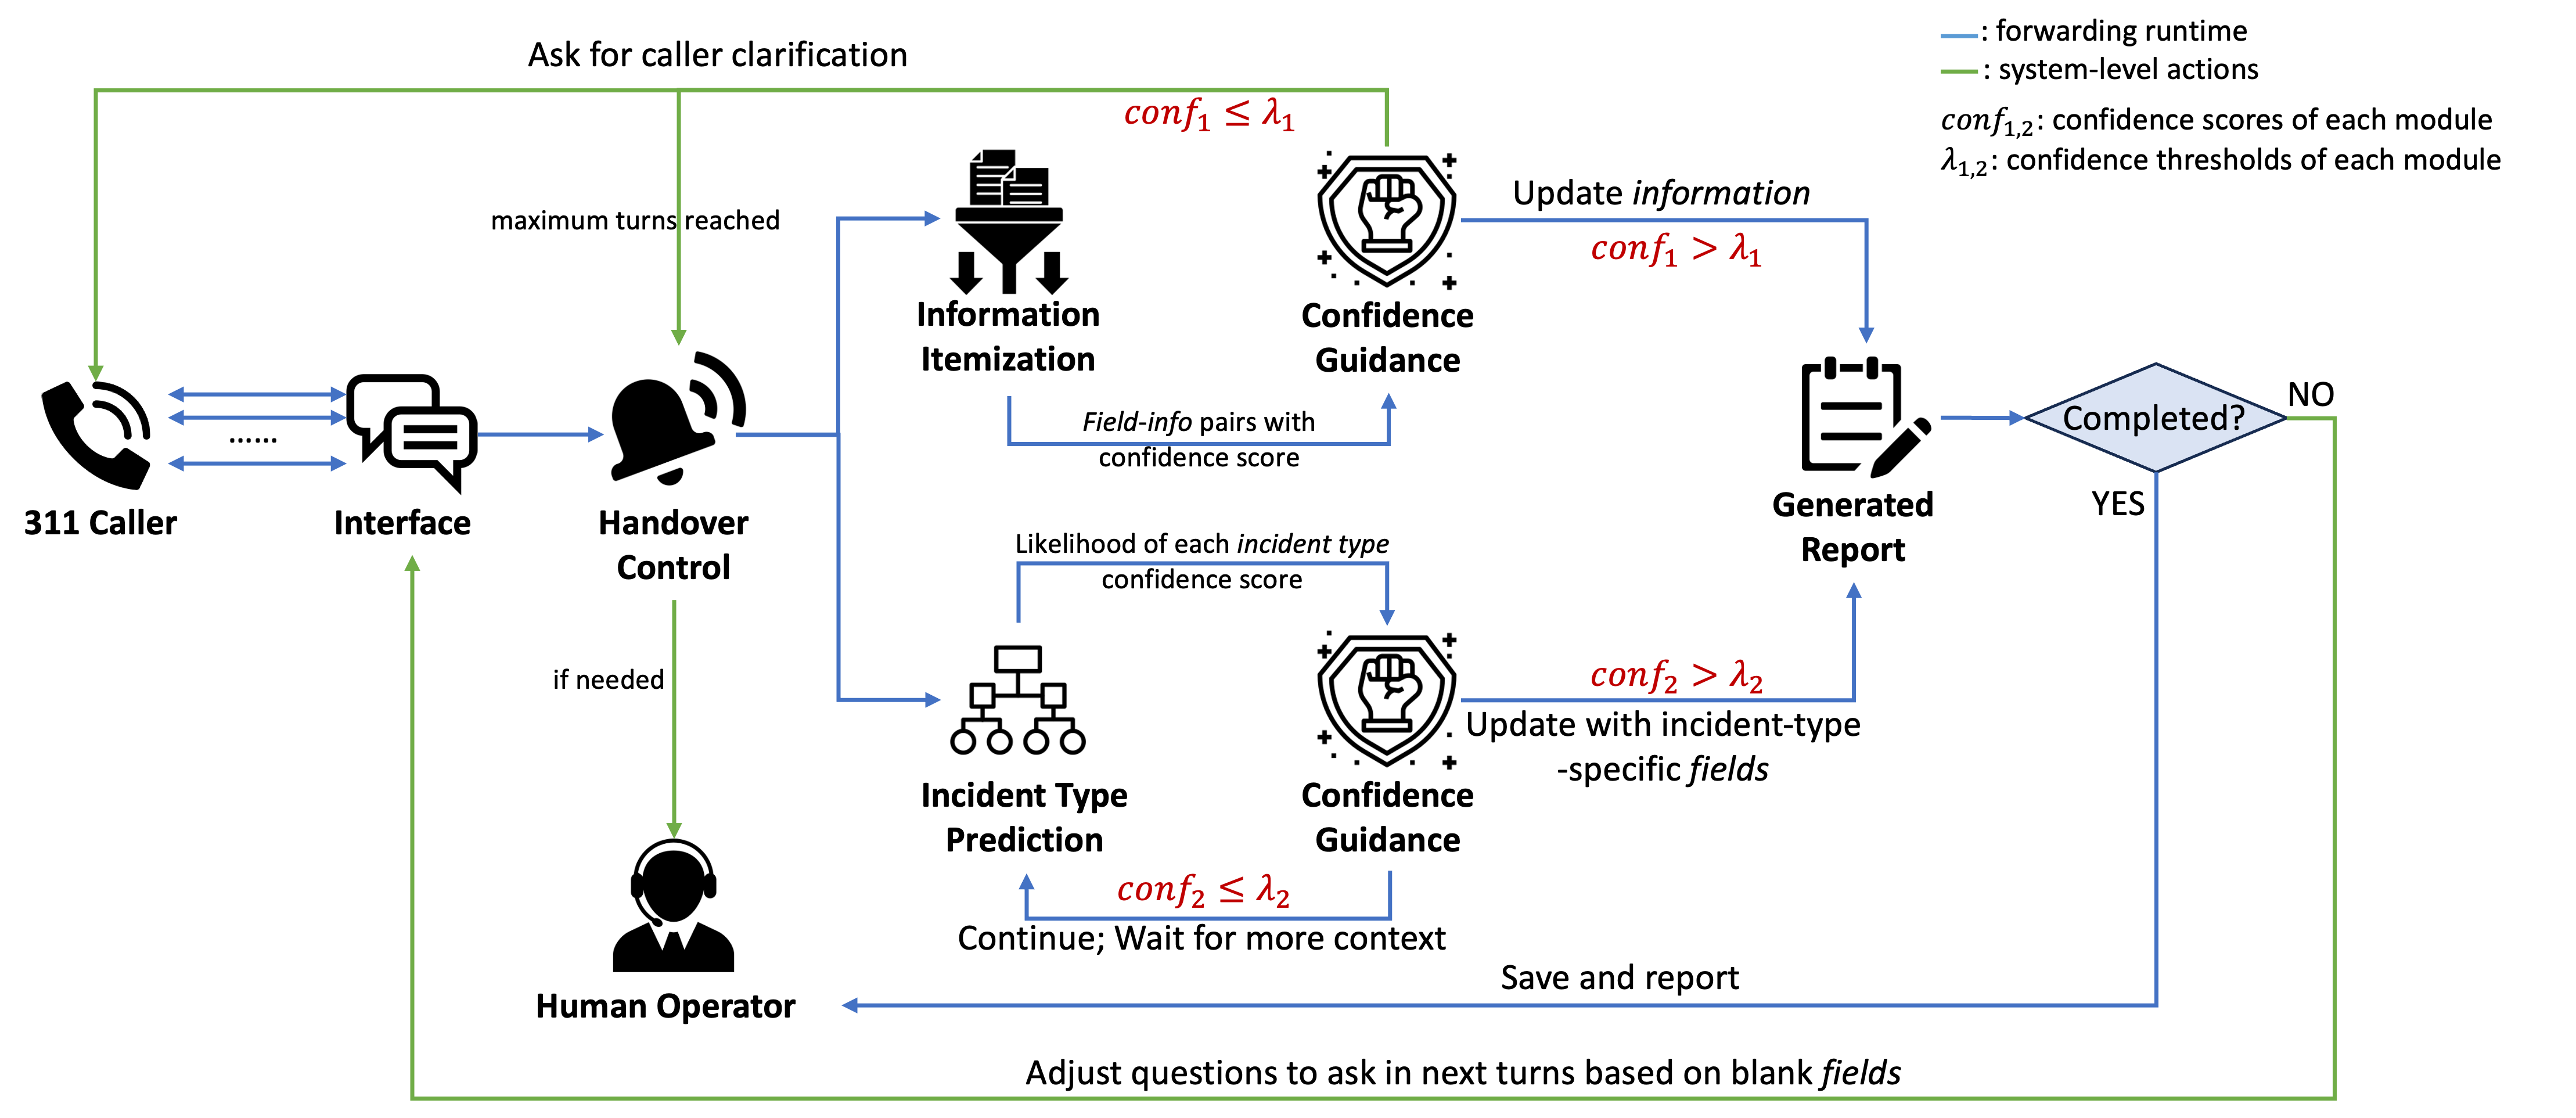
\includegraphics[width=0.9\textwidth]{figures/system_logic.png}
    \caption{Confidence-guided System Design}
    \label{fig:sys_logic}
    \vspace{-0.5cm}
\end{figure*}

% \subsubsection{Case Report vs Question List}
Importantly, the case report referred to here differs from the question list within the conversational interface. The question list stores upcoming inquiries for the interface, while the case report shapes the subsequent dialogue by updating the question list with its incomplete sections after each conversation turn.

% It is worth noting that the case report mentioned here is different from the question list in the conversational interface. The question list stores the next questions to ask for the conversational interface. However, the case report organizes the follow-up dialogue by updating the question list with its uncompleted fields after each conversation turn.

% in the following aspects: (1) the question list contains questions to ask in the next turns in the conversation, however, the case report consists of blank fields that need to be completed by the information itemization module; (2) the question list can be extended with blank fields with missing or low-confident answers while the case report can be extended by more specific fields under the predicted incident type from the incident type prediction module.

\subsection{Conversational Interface}

The conversational interface supports both voice and text inputs. Employing state-of-the-art audio transcription tools, notably the OpenAI Whisper model \cite{openai_whisper_2022}, this interface adeptly transforms speech into text, accommodating a range of accents. For text-to-speech functionality, we harness advanced audio generation tools like the Suno-AI Bark model \cite{bark}, acclaimed for producing realistic voices within a lightweight model framework. Beyond speech-to-text and text-to-speech conversion, the interface engages in conversations using a dynamically updated question list. This list determines the query sequence and guides the interface's speech-to-text conversion process.


% The conversational interface accommodates both voice and text formats. Leveraging cutting-edge audio transcription tools, specifically the OpenAI Whisper model \cite{openai_whisper_2022}, this interface proficiently converts speech to text while being adept at handling diverse accents. For text-to-speech generation, we rely on advanced audio generation tools such as the Suno-AI Bark model \cite{bark}, renowned for its capacity to produce remarkably realistic voices while maintaining a lightweight model size. Beyond the realm of text-to-speech and speech-to-text conversion, the conversational interface engages in interactions using a dynamically updated question list. This list dictates the sequence of questions to pose and serves as a guide for the interface's speech-to-text conversion process.

% The conversational interface supports both voice and text formats. Powered by one of the state-of-the-art audio transcription tools, the OpenAI Whisper model \cite{openai_whisper_2022}, the conversational interface is capable of speech-to-text transcription with robustness to different accents. Regarding backward text-to-speech generation, we also employ state-of-the-art audio generation tools, like the Suno-AI Bark model \cite{bark}, which guarantees highly realistic voice generation and light-weighted model size. Besides text-to-speech and speech-to-text generation, the conversational interface carries out the interactions with a question list that is dynamically updated each turn. The question list contains the next questions to ask and guides the speech-to-text generation of the interface. 

% In our settings, at the beginning stage, our interface initializes the conversation with the same opening question from a real operator: ``What is the location of the emergency?''. The starting question list only contains the following 4 questions: (1) what is the location of the emergency? (2) what is your name? (3) what is your best contact number? (4) Tell me what is going on. Then, the follow-up question list is generated at runtime based on the outputs from the next modules.

\subsection{Always-on Handover Control}

% The handover control module is kept active anytime during the runtime in case the current call needs to be rerouted to human operators. During our collaboration with the local call center, we further specify the following cases that trigger our handover control module: (1) when downstream modules return with exceptions, e.g., uncertain information; (2) when the caller keeps requesting to interact with a human operator, e.g., the caller says ``real operator'' or ``real human'' in the latest utterance; (3) early alerting for any potential urgency. The first case is handled inside system actions. For example, when Auto311 is uncertain about the itemized information, it asks the caller for clarification. We set the maximum turns of clarification to 3. Once the maximum is reached, we consider Auto311 faces exceptions and the handover control is triggered. To deal with the rest two cases, we develop an intuitive rule-based detection with high vigilance for future interpretability and control for the local call center team. We utilize Latent Dirichlet Allocation (LDA) \cite{blei2003latent} to produce a sensitive word list after manual review. We combine both nature language processing (NLP) features \cite{nltk} like stem, lemma, part-of-speech tags, and shallow parsing tags along with hand-coded patterns to figure out independent rules to trigger the handover control, ceasing system interaction. Please refer to the appendix for more details. Meanwhile, the patterns and sensitive words are not exhaustive; future usage expands the trigger conditions. However, this process goes beyond the scope of the current paper.

The handover control module remains active throughout runtime, redirecting calls to human operators when necessary. Collaborating with DEC, we identify specific scenarios that activate this module: (1) downstream module exceptions, like uncertain information; (2) caller's repeated request for human interaction; (3) proactive alerts for potential urgency. The first case is managed within system actions. For example, when Auto311 seeks clarification due to uncertain details, it limits such queries to three turns. Exceeding this threshold triggers exceptions and activates handover control. Addressing the other two cases, we develop an interpretable rule-based detection mechanism, prioritizing interpretability and control. Using Latent Dirichlet Allocation (LDA) \cite{blei2003latent}, we curate a sensitive word list through manual review. Our approach combines natural language processing (NLP) features \cite{nltk}, such as stemming, lemmatization, part-of-speech tags, and shallow parsing, with custom patterns to establish rules activating handover control, thus ending system interaction. More details are available in the appendix. Note that patterns and sensitive words are not exhaustive, allowing future expansion of trigger conditions. However, the broader process is beyond this paper's scope.

% The handover control module remains active throughout runtime to reroute calls to human operators as needed. Collaboration with the local call center leads us to identify specific scenarios that activate this module: (1) when downstream modules encounter exceptions, such as uncertain information; (2) when the caller repeatedly expresses a desire to communicate with a human operator; (3) proactive alerting for potential urgency. The first case is managed within system actions. For instance, when Auto311 is uncertain about detailed information, it seeks clarification from the caller, limiting such queries to three turns. If this threshold is reached, Auto311 deems exceptions present and triggers the handover control. To address the other two cases, we've developed an easily interpretable rule-based detection mechanism with a strong focus on future interpretability and  control. Employing Latent Dirichlet Allocation (LDA) \cite{blei2003latent}, we curate a sensitive word list via manual review. Our approach combines natural language processing (NLP) features \cite{nltk}, such as stemming, lemmatization, part-of-speech tags, and shallow parsing, with custom-coded patterns to establish distinct rules that activate the handover control, thus discontinuing system interaction. Further details are available in the appendix. It's important to note that the patterns and sensitive words are not exhaustive, leaving room for the expansion of trigger conditions in future applications. However, this broader process falls outside the scope of this paper.

\subsection{Incident Type Prediction}
\label{subsec:prediction}

The incident type prediction module utilizes contextual information from previous caller utterances. The module takes the overall context covering all prior utterances as input. Since a context can involve multiple incident types, we apply a multi-layer hierarchical structure and bootstrap-like procedure for classification. This tracks the possibility of the call belonging to each incident type (see Confidence-guided System Design for details). The hierarchical structure and iterative procedure enable the prediction module to handle multiple incident types per call using full conversational context.

% The contextual information from previous utterances facilitates the incident type prediction module. The module input is the overall context covering all previous caller utterances. Considering it is possible for a context to involve more than more incident types, we apply a multi-layer hierarchy structure and a bootstrap-like procedure for this classification to keep track of the possibility of the call belonging to each incident type, refer to more details in Section Methodology.

\subsection{Information Itemization}
\label{subsec:itemization}

The information itemization module completes empty case report sections by quoting the caller's utterances. This involves narrative fields seeking explanatory details and yes/no fields confirming facts. For narratives, we leverage extractive question-answering frameworks - the blank fields are inputs, and outputs quote relevant caller utterances. Yes/no fields become binary classification, predicting yes or no from the last utterance. Unlike incident prediction using all contexts, itemization considers only the latest utterance. 

% The information itemization module has a specific goal: to complete the empty sections in a case report quoting information from what the caller says. This involves two main types of fields: one that asks for a narrative explanation, such as where the incident happened, and another that seeks a simple ``yes'' or ``no'' based on what the caller says, like ``Are you the property owner?''. To deal with the first type, leveraging the ability of existing extractive question-answering frameworks, this module takes the blank fields in the case report as input and outputs the most relevant information by quoting the caller utterance segments. Meanwhile, we formulate the second type as a binary classification task. Different from the incident type prediction, which considers all previous contexts, this information itemization module considers only the last caller utterance as context. 

% Before the model is trained, we thoroughly examine our dataset and the local call center's guidelines for various incident types. We annotate the audio transcriptions to form our dataset in field-information pairs, which enables the training of this module. Different from the incident type prediction, which considers all previous contexts, this information itemization module considers only the last caller utterance as context. 

\subsection{Confidence-guided Report Generation and Dialogue Optimization}

This module updates the report and optimizes dialogues as the conversation progresses. See technical details in Section Confidence-guided System Design.

% The iterative report optimization and dialogue assistance allow dynamically improving reports as the conversation progresses.

% This module targets the optimization of the generated case report during every turn of the ongoing conversation and further assists dialogue organization. We discuss more technical details in Section Confidence-guided System Design.


% Our system assists dispatchers by suggesting likely incident types and itemizing key information to answer essential case report questions. The system, depicted in Fig. \ref{fig:sys_overview}, comprises incident type prediction and information itemization modules. It does not participate directly in dispatcher-caller conversations; rather, it generates an evolving answer sheet for dispatcher review and revision during the interaction. Fig. \ref{fig:running_example} demonstrates module cooperation within a single conversation turn, showcasing assistance for dispatchers.

% % Our system is designed to assist the dispatchers by (1) suggesting the most likely incident type of the ongoing call and (2) highlighting key information that would potentially answer the essential questions to file an internal case report. Thus, besides the handover control, there are two main modules in our system, see Fig.\ref{fig:sys_overview}: call dispatching and information extracting. Our system does not directly participate in the conversation between the dispatcher and the caller, it aims to generate an answer sheet for the dispatcher every turn as the conversation goes on, and the dispatcher has full access to review and revise the answer sheet anytime during the conversation. To better demonstrate how these two modules help with the dispatcher and interact with each other, we provide a running example, see Fig.\ref{fig:running_example} within one single turn of the conversation.

% Given previous findings on potential urgent situations underlying calls, we develop a \textbf{handover control} that interrupts system interference and routes the call to the dispatcher when more urgent incidents are detected, acknowledging each call's severity.

% % Based on the findings in the previous section, we acknowledge the potentially life-threatening situation behind each call, We develop a \textbf{handover control} in case the ongoing call is identified as an emergency call instead. The handover control interrupts the interference from our system and leaves the dispatcher the only participant during the call once there is any sign of an emergency is detected.

% \subsection{Call Dispatching Module}

% We track user utterances, maintaining overall context information passed to the call dispatching module. This multi-class classification module outputs the likelihood of categorizing the call into each incident type. The final prediction assists rather than replaces the dispatcher's decision-making, with the dispatcher retaining full control to alter outputs. The most likely incident-type queries associated with follow-up questions from the DEC question card, e.g., ``What is the vehicle color?'' for abandoned vehicles. These questions are appended to the information extracting module's question list.

% % During the call, we track every user utterance and maintain overall context information. The context information is passed to the call dispatching module. We model the whole process as a multi-class \textbf{classification} task and train the module to output the likelihood of whether the current call should be categorized into each incident type. The final prediction is provided to the dispatcher in a soft way, which means it only aims to assist the decision maker (dispatcher) instead of being the decision maker. Meanwhile, the dispatcher has full control over the module and can change the output anytime during runtime. After having the most likely incident type, this module queries all the follow-up questions from the DEC's question card specifically under that incident type, e.g., ``what is the color of the vehicle?'' under the abandoned vehicle category. Those follow-up questions are passed and appended to the question list in the information extracting module.

% \subsection{Information Extracting Module}

% The information extracting module focuses on extracting key information from the latest utterance to fulfill the essential questionnaire for internal reports. We model this as a QA pipeline trained to mark start and end indices in an utterance to answer a given question. The question list contains essential questions, starting with common questions before incident types are confirmed. Once confirmed, incident-specific questions are added, enabling the handling of additional caller-volunteered information. If there is only one single possible incident type confirmed, we will only query that certain incident type and follow DEC's question card, which contains all procedural questions that need to be further answered to complete the report. If there are multiple incident types detected, the question list will be updated using all relevant questions belonging to the detected incident types. Our confidence-checking functions make sure only the incident type(s) and its corresponding question-answer pairs with high internal consistency will be reported to the dispatcher.

% % The information extracting module mainly focuses on the latest user utterance and attempts to extract the key information from the latest utterance to fulfill the questionnaire that is essential to complete an internal report. We model the process as a \textbf{Q\&A-like pipeline}. This module is trained to mark the start and end indices in a given utterance to answer a given question. Meanwhile, the question is not limited to the proposed question by the dispatcher. Based on the findings from the previous section, there is a chance that the caller could convey additional information during the conversation, thus, we set up a question list for essential questions to ask. At initial turns, or before an incident type is confirmed, the question list only consists of common questions, which are not specific to any of the incident types. Once the incident type is confirmed, the question list will be extended with more incident-specific questions.

% \subsection{Confidence Checking Function}
% Confidence checking participates in both key modules, providing predictions and confidence scores indicating certainty. Low confidence suggests dispatchers carefully consider adopting predictions. We develop rules during runtime to strategically utilize the confidence scores. At the system level, the implementation of several procedural rules allows our system to make confidence-aware choices aimed at maximizing overall confidence scores throughout the conversation. In Fig. \ref{fig:dryrun}, further explanation elucidates confidence checking's system influence. Initially, system interactions initialize with the human operator's opening question: ``What is your emergency location?''. Concurrently, the question list commences with this location query alongside other questions commonly imperative for most incident types. Post-questioning, the system awaits and analyzes caller utterances for contextual information. Leveraging context, both modules generate predictions and associated confidence scores. Parallel module-specific methods determine prediction-confidence adoption. For information extraction, firm adoption only occurs for question-answer pairs exceeding the confidence threshold; clarification requests elicit below-threshold pairs until exceeding the threshold. Similarly, the call dispatching module only accepts the incident type and then updates the question list using retrieved incident-specific questions given sufficient confidence. However, immediate clarification does not occur. Instead, the system remains silent until all question list queries receive answers. Absent an identified most probable incident type(s) at that juncture prompts caller solicitation of an incident narrative description and suggests human operator callback in case of insufficient assertion of incident type from the current answer sheet.

% % we further explain how the confidence checking method influences the system choices. At the beginning stage of a conversation, our system initializes the interactions with the same question that is asked by human operators: ``What is the location of your emergency?''. Meanwhile, the question list starts with not only this question querying the location information but also with other questions that are commonly important to answer in most incident types. After the question is proposed, our system waits and listens to the caller's utterances to obtain the context information. Based on the context information, both modules output predictions along with corresponding confidence scores. We apply different methods to decide whether to adopt each of the prediction-confidence pairs in two modules in parallel. In the information extracting module, once question-answer pairs and their confidence scores are obtained, our system only firmly adopts those pairs with a confidence higher than the threshold. If question-answer pairs do not achieve a high enough confidence score, our system asks the user to clarify the answers until the score exceeds the threshold. In the call dispatching module, similar to the information extracting module, our system only accepts the incident type and then updates the question list using retrieved questions under the predicted incident types. However, our system does not immediately asks for clarification, instead, our system keeps silent until all the questions in the question list are answered. If our system still does not figure out the most likely incident type(s) by then, the caller will be asked to provide a narrative description of the ongoing incident and human operators will be suggested to make a callback in case the currently generated answer sheet is not enough to assert an incident type.

% % \begin{figure*}[t]
% %     \centering
% %     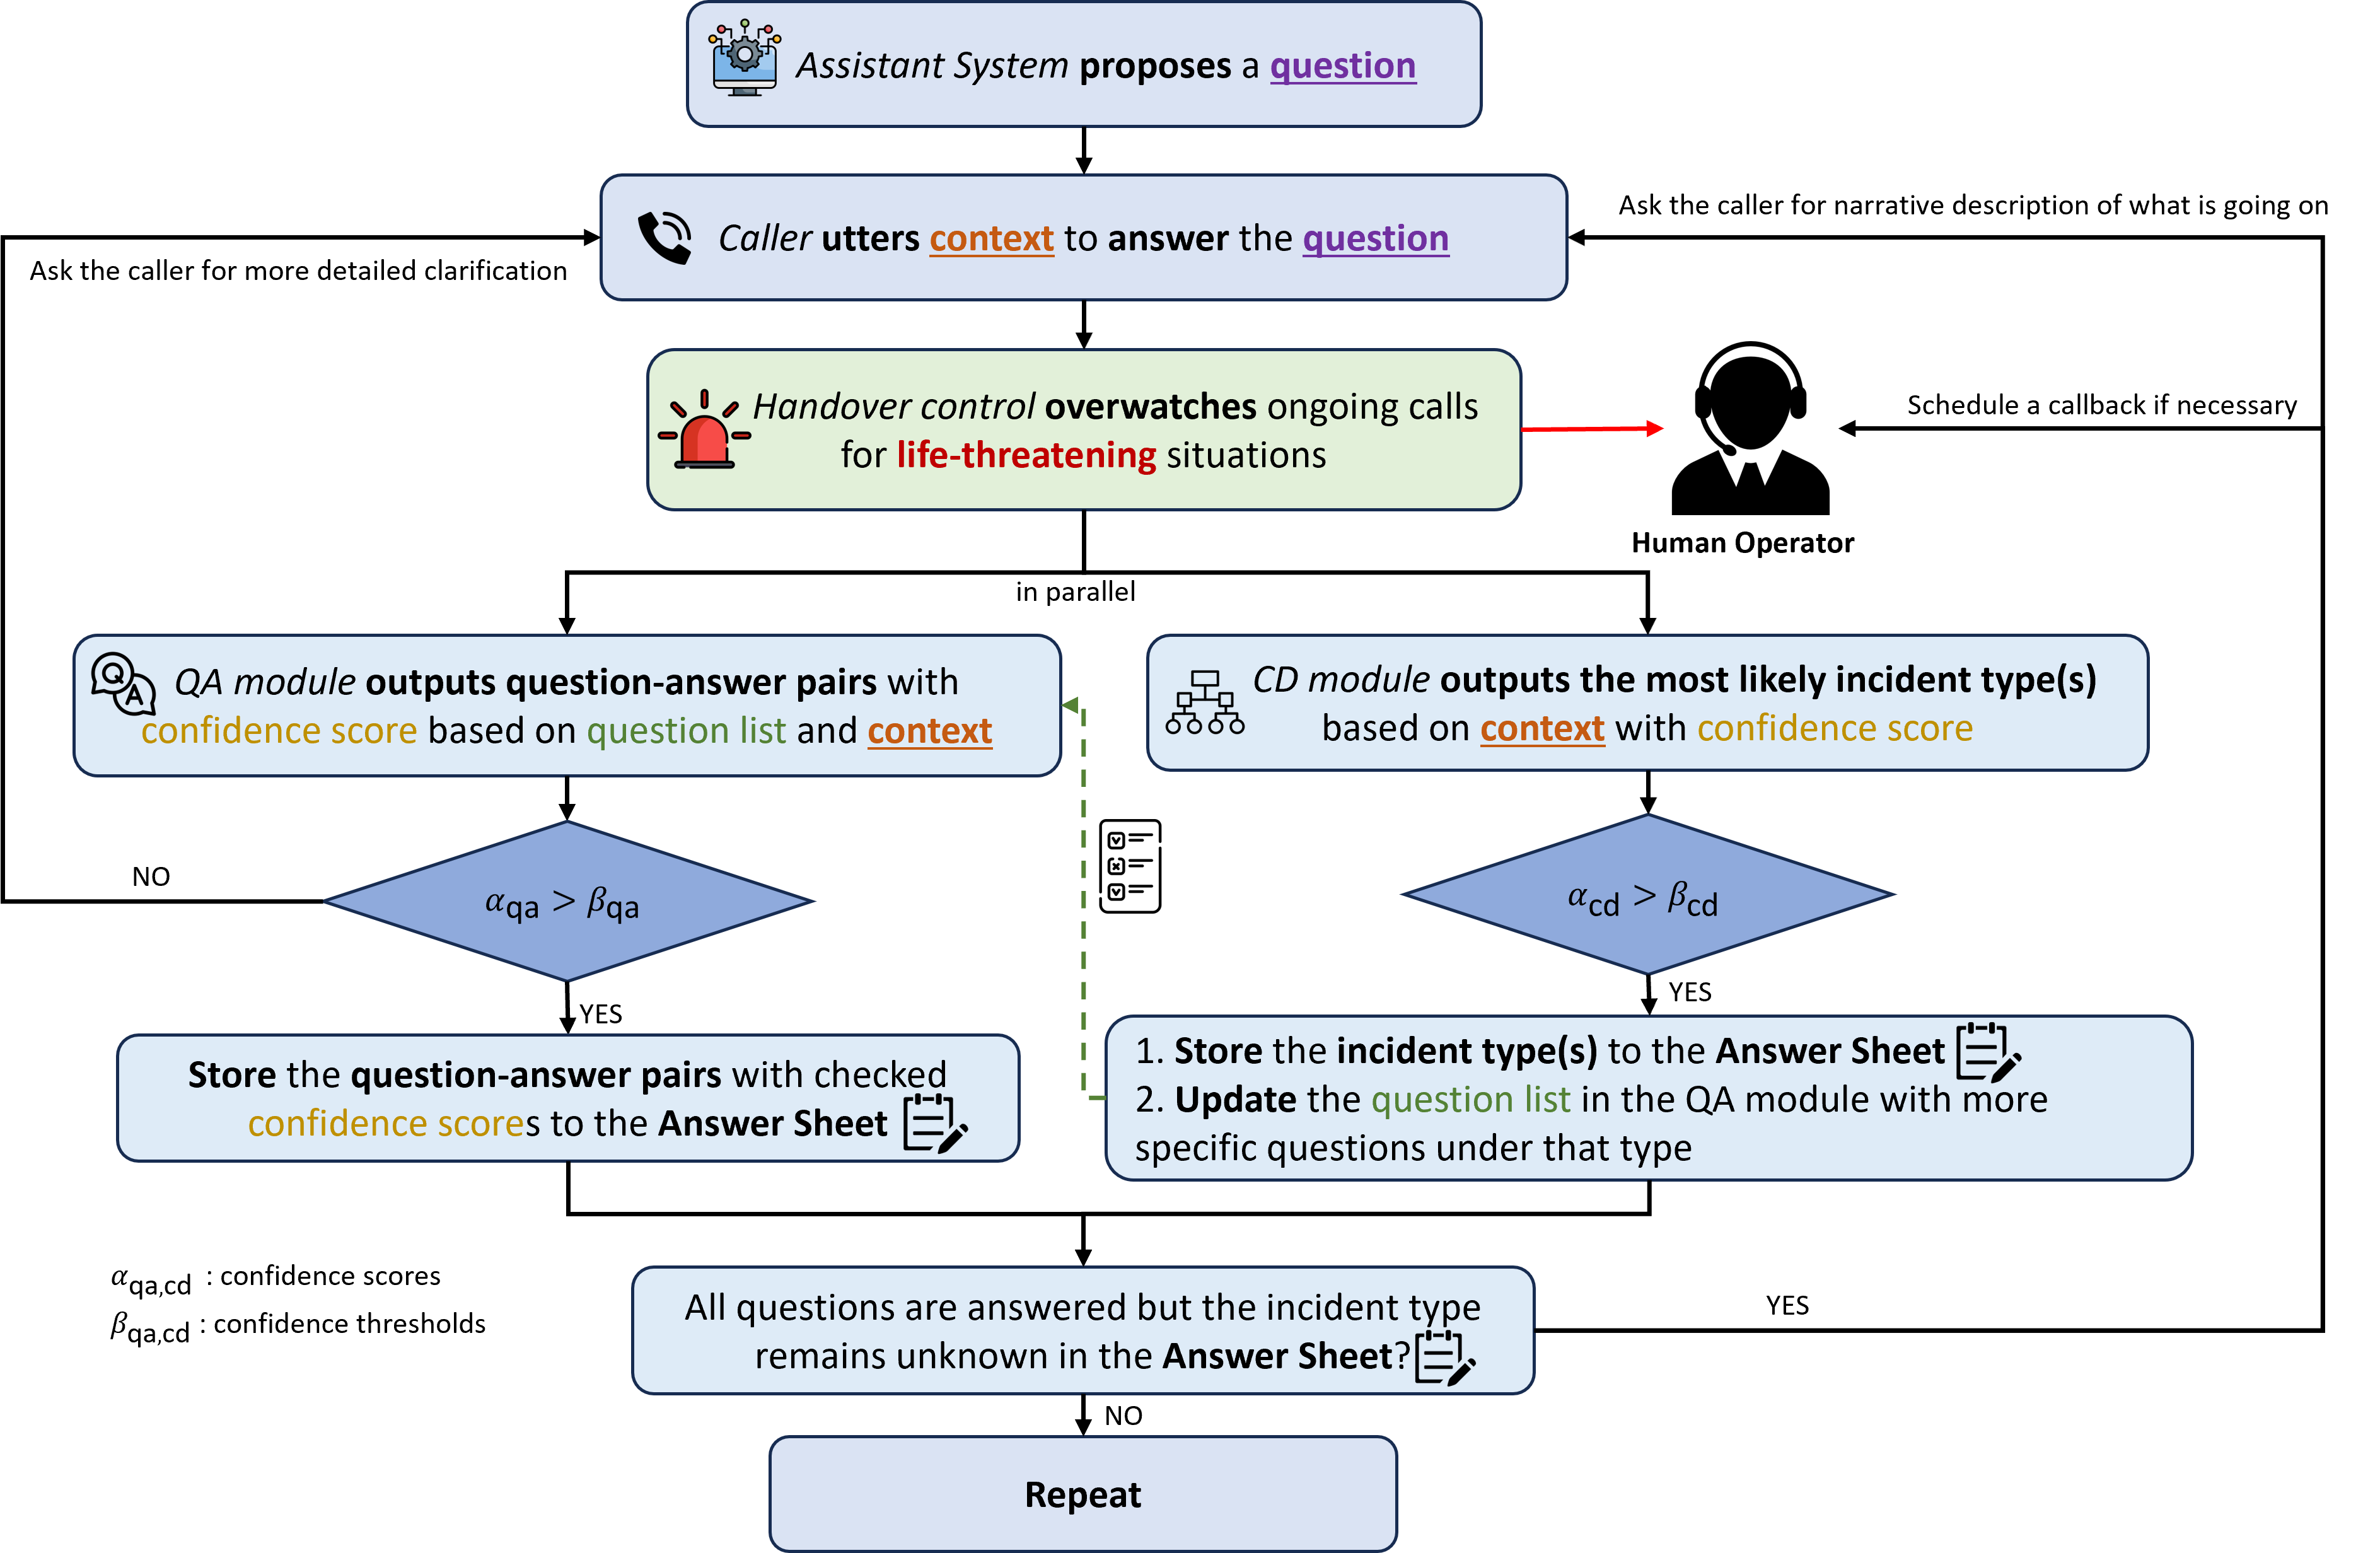
\includegraphics[width=0.9\textwidth]{figures/system_dryrun.png}
% %     \caption{Confidence-aware system choices}
% %     \label{fig:dryrun}
% %     \vspace{-0.5cm}
% % \end{figure*}


% % Confidence checking participates in both of the key modules. This module aims to not only provide the predictions to the dispatcher but also to include a \textbf{confidence score} which, by our design, indicates how the modules are confident with current outputs. A low confidence score might suggest the dispatcher carefully deciding whether to adopt the predictions.

\section{Confidence-guided System Design}

This section delves into the technical aspects of confidence guidance within Auto311. Firstly, we explain the method to derive confidence scores from the machine learning models. Secondly, we elucidate the purpose of the generated confidence scores within the workflow.

% In this section, we discuss the technical details of the confidence guidance in Auto311. First, we explain the applied method to obtain the confidence score behind the machine learning models. Second, we illustrate the role of the generated confidence scores in the workflow.

\begin{figure*}[t]
    \centering
    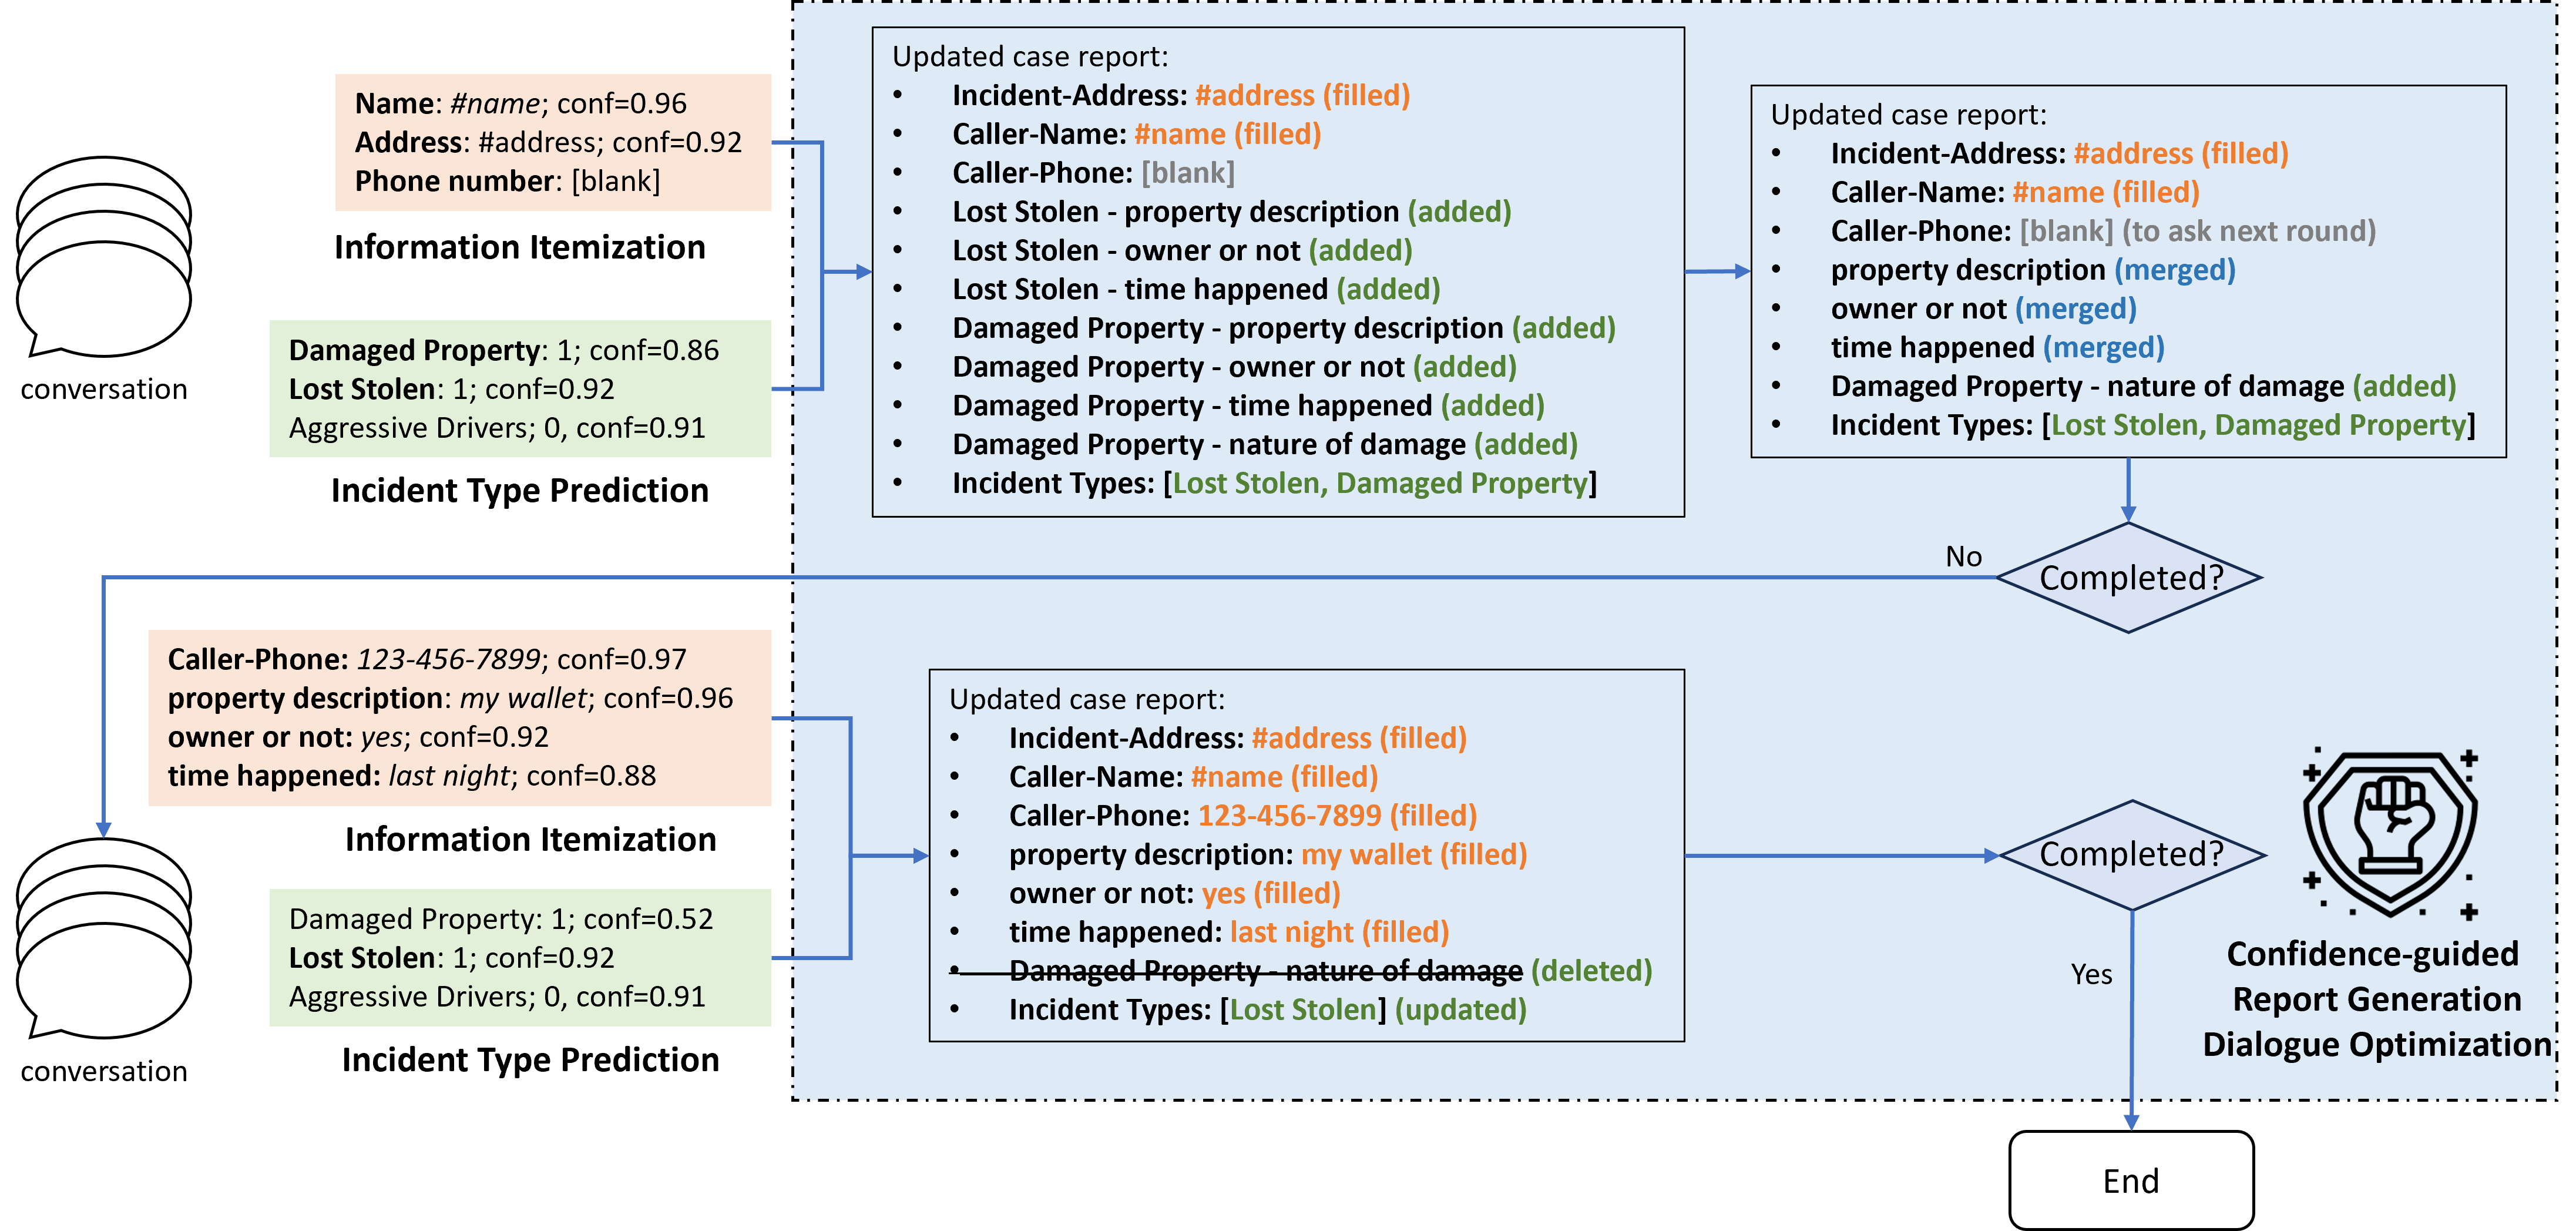
\includegraphics[width=0.9\textwidth]{figures/case_study.png}
    \caption{A General Case Study in Confidence Guidance}
    \label{fig:case_study}
    \vspace{-0.5cm}
\end{figure*}

\subsection{Confidence Measurement}

We define confidence as consistency over multiple trials with the same inputs. We leverage Monte Carlo Dropout\cite{gal2016dropout, ma2021predictive} to generate the confidence prediction. Specifically, dropout was set as active at test time and assesses consistency across trials to obtain scores. Preset thresholds determine if outputs are confident - meeting or exceeding the threshold means confident. Auto311 applies machine learning models to handle two major tasks component-wisely: incident type prediction and information itemization. Here we detail Auto311's approach to measuring confidence.

% Following the definition of confidence score in machine learning as ``the internal consistency with same input after multiple trials'', we apply a similar structure in \cite{ma2021predictive} -- leaving the dropout layer active during testing and calculating the consistency over multiple trials to obtain a confidence score. We set up confidence thresholds -- if the confidence score remains at the threshold or higher, the output is deemed confident. Auto311 applies machine learning models to handle two major tasks component-wisely: incident type prediction and information itemization. Here we detail Auto311's approach to measuring confidence.

\subsubsection{Confidence in Incident Type Prediction}

To address potential multiple incident types within a call, we employ a multi-layer hierarchy structure coupled with a bootstrap-like process. The initial layer of this structure involves training a neural network to assess if the present context corresponds to the most common incident type. Subsequently, the second layer trains another neural network to determine if the context aligns with the second most frequent incident type, excluding the previously identified type. This pattern continues for subsequent types. As a result, (1) the structure can identify all possible incident types within a call; (2) each category operates independently, facilitating future adjustments based on new data or expansion to more categories. At runtime, we establish confidence scores by measuring consistency across output distributions for the same input, utilizing active dropout to quantify prediction uncertainty. The hierarchical cascade structure adeptly handles multiple types, while confidence scoring measures prediction certainty.

% To handle the potential multiple incident types in each call, we apply a multi-layer hierarchy structure with a bootstrap-like procedure. The first layer of the multi-layer classification structure contains a neural network trained to determine if the current context belongs to the most prevalent incident type. Subsequently, the second layer involves training a separate neural network to ascertain if the current context corresponds to the incident type with the second highest frequency after excluding the previous type from the training set, continuing in this manner. Consequently, (1) the overall structure can identify all potential incident types from an ongoing call; (2) each category avoids interfering with others, enabling future fine-tuning on new data samples or expansion with additional categories. We obtain confidence scores at runtime by measuring consistency among output distributions with the same input, keeping dropout active. This quantifies uncertainty in the predictions. The hierarchical cascade structure flexibly handles multiple types, while the confidence scoring quantifies prediction certainty.

\subsubsection{Confidence in Information Itemization}

% Drawing from the machine learning concept of a confidence score, defined as the consistency when testing the same input multiple times, we adopt a similar approach as seen in \cite{ma2021predictive}. This involves keeping the dropout layer active during testing, calculating consistency across multiple trials, and deriving a confidence score. We establish confidence thresholds: if the score equals or surpasses the threshold, the output is considered confident. Auto311 employs machine learning models for two key tasks: predicting incident types and handling information itemization. In this context, we elaborate on how Auto311 gauges the confidence for each task component.

Regarding textual outputs for information itemization, determining confidence necessitates a consistency assessment between texts. Traditional text comparison methods often prioritize aspects like edit distances and length. See details in Related Work. However, our collaboration with DEC underscores the value of succinct outputs with ample details for case reports. Consider the scenario where the module generates ``on the 2525 West End Ave'' while the ground truth is ``2525 West End Ave.'' Traditional methods yield low scores, such as 0.5 from BLEU-bigram. However, when dispatchers gather incident location details, these outputs should exhibit high consistency due to matching location keywords and similar semantics. To address this, we adopt a new approach. For keywords, we employ an unsupervised state-of-the-art keyword extractor \cite{campos2018yake} to extract key segments from model outputs. The overlap between keyword segment lists is calculated. For semantics, we utilize SentenceBERT \cite{reimers-2019-sentence-bert} to project each output into a latent space, assessing the similarity between represented textual string lists. The overall score, calculated via Polyak averaging (p=0.2), integrates keyword overlaps and embedding distances. This metric enables us to gauge consistency and generate a confidence score.

% When it comes to textual outputs in information itemization, it first requires a method to calculate the consistency between texts before a confidence score is finally measured. Traditional text comparison approaches primarily emphasize features including edit distances and length. But throughout the collaboration with the local call center team, we consider concise outputs with ample details more useful for information itemization in the case report. For instance, if the module generates ``on the 2525 West End Ave'' but the ground truth is ``2525 West End Ave'', traditional text comparison methods furnish low scores, e.g. 0.5 from BLEU-bigram. Critically, when dispatchers gather incident location information, these outputs should exhibit high consistency since both contain identical location keywords and similar semantics. Thus, here, for keywords, we leverage an unsupervised state-of-the-art keyword extractor \cite{campos2018yake} to extract key segments from model outputs and calculate the overlap between keyword segment lists. For semantics, we apply SentenceBERT \cite{reimers-2019-sentence-bert} to project each output into a latent space, calculating the similarity between represented textual string lists. The overall score calculates using Polyak averaging, p=0.2, based on keyword overlaps and embedding distances. With the help of the text comparison metric, consistency now can be obtained and a confidence score can be generated under this scenario.

\subsection{Report Generation and Dialogue Optimization}

Auto311 is designed to be confidence-guided. With maximum confidence guaranteed, it (1) dynamically updates case reports at every turn of the conversation and (2) guides the follow-up conversation based on the generated case report. See Figure \ref{fig:sys_logic} for more detailed system logic. 

Confidence drives precise report completion via information itemization. Using the latest caller utterance, it populates report details. Textual output confidence is determined through text comparison. As in Figure \ref{fig:sys_logic}, uncertainty ($conf_1 \leq \lambda_1$) prompts Auto311 to seek clarification for guiding questions, capped at three turns before handover control. Confidence ($conf_1 > \lambda_1$) skips further dialogue optimization for filled fields. Confidence also aids the incident type prediction module's adaptability and report efficiency. Using complete utterance context, it predicts likely incident types. As shown in Figure \ref{fig:sys_logic}, low confidence ($conf_2 \leq \lambda_2$) excludes uncertain predictions from reports. High confidence ($conf_2 > \lambda_2$) incorporates predictions. Systemically, prediction persists each turn, even post early confident identification. This iterative process tracks trends in types and scores, updating reports on confidence drops ($conf_2 \leq \lambda_2$). Confidence-driven adaptation detects and responds to evolving incident types during calls, further updating reports.

% Confidence guides high-quality case report completion through information itemization. Taking the latest caller utterance, it outputs details for relevant report fields. As explained, text comparison determines confidence for textual outputs. As shown in Figure \ref{fig:sys_logic}, if uncertain about itemized info ($conf_1 \leq \lambda_1$), Auto311 prompts clarification if fields guide subsequent questions, capped at 3 turns before handover control is triggered and an operator steps in. When confident ($conf_1 > \lambda_1$), filled fields are excluded from further dialogue optimization. Confidence quantification thus optimizes itemization to complete reports more effectively.

% Confidence is a key factor guiding the accurate completion of case reports through information itemization. The module takes the most recent caller utterance as input and produces itemized information for the relevant fields in the case report as output. As explained earlier, the confidence score for text-based outputs is determined through text comparison. If Auto311 lacks certainty about the itemized information, it prompts the caller for clarification when $conf_1 \leq \lambda_1$, provided the fields guide subsequent questions. Our system limits caller clarification to three turns at most, after which a live operator steps in. Conversely, when $conf_1 > \lambda_1$, Auto311 is confident in the provided itemized information, leading to the fulfillment of the answered fields and exclusion from future dialogue optimization.



% Confidence also enables the incident type prediction module to adapt to evolving categories and generate reports more effectively. Taking the full utterance context, it predicts the most likely types. As illustrated in Figure \ref{fig:sys_logic}, low confidence scores ($conf_2 \leq \lambda_2$) mean uncertainty, so those predictions are excluded from report generation. High confidence ($conf_2 > \lambda_2$) incorporates predicted types into created reports. At a system level, prediction stays engaged every turn, even after confident early identification. This iterative checking empowers Auto311 to monitor trends in types and scores - a drop ($conf_2 \leq \lambda_2$) triggers excluding fields tied to uncertain types, updating the report. Confidence-guided adaptation allows detecting and responding to shifting incident types during the call to further update reports.

% Confidence serves as a guiding principle for the incident type prediction module, allowing it to dynamically adapt to evolving incident categories and generate case reports more effectively. The module takes the overall utterance as input and produces the most likely incident type(s) as output. When Auto311 predicts incident types with a confidence score below the threshold $conf_2 \leq \lambda_2$, it signifies uncertainty in the prediction. Consequently, such predictions are not incorporated into the report-generation process. Conversely, when $conf_2 > \lambda_2$, the predicted incident types are used to generate case reports with specific fields tailored to those types. At a system level, Auto311 maintains the incident type prediction module's engagement in every conversational turn to ensure awareness of the ongoing context. This holds true even when earlier turns have confidently identified an incident type. This approach empowers Auto311 to monitor trends in incident types and their corresponding confidence scores. If the confidence score drops below the threshold ($conf_2 \leq \lambda_2$), indicating decreased certainty in the incident type prediction, Auto311 adjusts the case report by excluding fields highly tied to the specific incident type. This ability allows Auto311 to detect and respond to changes in caller-identified incident types during the conversation, thus updating the case report accordingly.

% Confidence guides the incident type prediction module to dynamically adjust to the shifting incident types and more appropriately generate the case report. The input of the incident type prediction module is the overall caller utterance and the output is the most likely incident type(s). When Auto311 predicts the incident types with a low confidence score $conf_2 \leq \lambda_2$, it implies Auto311 is not fully certain about the prediction. In this case, the prediction is not adopted for report generation. Oppositely, when $conf_2 > \lambda_2$, the predicted incident types are further utilized to generate the case report with type-specific fields. Meanwhile, at a system level, Auto311 keeps the incident type prediction module active at every turn of the conversation to make it aware of the overall context, even when previous turns have confirmed one incident type with a high confidence score. By doing so, Auto311 is capable of tracking the trend of both incident types and the corresponding confidence scores. If the confidence score decreases lower than the threshold, when $conf_2 \leq \lambda_2$, indicating the incident type prediction module is no longer certain about the given type, Auto311 modifies the case report by dropping fields highly specific to the incident type. Thus, when the caller shifts the incident types during the call, Auto311 detects the shift and adjusts the case report using the updated incident type.

Previous component confidence scores further optimize future dialogues. In the case study illustrated in Figure \ref{fig:case_study}, when a new caller utterance is received, Auto311 identifies fields to complete in the case report (e.g., incident-address, caller-name, caller-phone). High-confidence completion marks them as done. Unfinished fields guide subsequent questions (e.g., requesting a callback number if caller-phone is missing). Concurrently, incident type is confirmed if confidence surpasses a set threshold (0.85 in Figure \ref{fig:case_study}). With the type established, specialized fields are identified (e.g., property description for lost/stolen cases), updating the report. Auto311 then prioritizes shared general fields (e.g., property description, time, ownership status), streamlining dialogue to focus initially on universal details. This avoids asking about the damage nature before finalizing the incident type, which applies only to damaged property cases. This optimization confirms type(s) with more context. In the example, the next turn's details indicate a shift to "lost/stolen" only. The report is updated accordingly. The dialogue concludes when all report fields are complete. Confidence scoring thus optimizes the flow by collecting universal details first and adapting to emergent incident types.


% The confidence scores from previous components play a significant role in optimizing future dialogue. As illustrated in the case study \ref{fig:case_study}, when receiving a new caller utterance, Auto311 first identifies fields to fill in the case report (e.g. incident-address, caller-name, caller-phone). High confidence completion of these fields marks them as finished. Remaining incomplete fields guide the next questions (e.g. asking for callback number if caller-phone is missing). Simultaneously, the incident type is confirmed if its confidence exceeds a preset threshold (0.85 in the figure). With the type established, Auto311 identifies specialized fields needed (e.g. property description for lost/stolen cases). The report is updated accordingly. Following this, Auto311 consolidates and prioritizes more general fields shared across incident types (e.g. property description, time, ownership status). This streamlines the dialogue to focus initially on universal information before specific inquiries. For instance, the system avoids asking about the nature of damage before finalizing the incident type, since it is identical to only damaged property cases. This optimization provides additional context to confirm type(s). In the example, in the next turn, the caller supplies missing details that indicate shifting to ``lost/stolen'' only. The report is updated based on the revised predictions. The dialogue concludes when all report fields are complete. In summary, confidence scoring enables optimizing the flow to gather universal details first, then adapt based on emergent incident types.

% The confidence scores produced by the previous components play a significant role in optimizing future dialogue, as illustrated in a general case study in Figure \ref{fig:case_study}. Upon receiving a new caller utterance, Auto311 initially identifies the fields that need to be filled in the case report. For example, in Figure \ref{fig:case_study}, these could include incident-address, caller-name, and caller-phone. If these pieces of information are collected with high confidence, the corresponding fields are marked as completed. The fields that remain incomplete guide the ongoing conversation, determining the next questions to be posed. For instance, if caller-phone is missing (as indicated by the gray marking in the figure), the next question might be, ``What is your preferred callback number?'' Simultaneously, the incident type is confirmed if its confidence score surpasses the preset threshold, represented as 0.85 in Figure \ref{fig:case_study}. Once the incident type is established, Auto311 refers to the call center's protocol to identify fields requiring type-specific details. In the figure, the prevalent incident types are ``damaged property'' and ``lost/stolen property.'' Accordingly, the case report is augmented with specialized fields such as ``lost stolen - property description'' and ``damaged property - nature of damage.'' Following this update, Auto311 proceeds to consolidate and prioritize less specific fields. For instance, both ``damaged property'' and ``lost stolen property'' incidents necessitate common information like property description, time of occurrence, and ownership status. Hence, Auto311 combines and gives priority to these shared fields. The outcome is a more streamlined dialogue that initially focuses on gathering universal information, postponing highly specific inquiries until incident types are definitively determined. For example, as shown in the second turn of Figure \ref{fig:case_study}, the system avoids inquiring about the nature of damage before the incident type is finalized. This optimized dialogue approach also affords Auto311 additional context to confirm the incident type(s). In the subsequent turn of conversation depicted in Figure \ref{fig:case_study}, the caller not only supplies the missing phone number but also provides details about the related property and the time of the incident. This new information indicates a shift in incident type to ``lost stolen'' only. Consequently, the case report is updated based on the revised module outputs. The dialogue concludes when all fields in the case report are filled.

% The confidence emitted by the components is also utilized for future dialogue optimization, see a general case study in Figure \ref{fig:case_study}. Once a new caller utterance is given, Auto311 first tracks the fields to complete in the case report, e.g., incident-address, caller-name, and caller-phone in Figure \ref{fig:case_study}.  If that information is collected with high confidence, the corresponding fields are marked as completed. The uncompleted fields guide the dialogue by defining the next questions to ask in future turns, e.g., caller-phone is missing, marked grey, and the next question to ask is ``What is your best number for a callback?''. At the same time, the incident type is confirmed if the confidence score exceeds the threshold, set to 0.85 in Figure \ref{fig:case_study}. Once the incident type is confirmed, Auto311 refers to the call center's protocol for fields with type-specific information. As shown in the figure, the most incident types are damaged property and lost/stolen property. Thus, the case report is updated with additional specific fields like the ``lost stolen - property description'' and ``damaged property - nature of damage''. After updating the case report, Auto311 updates the case report by merging and prioritizing less specific fields. For example, in Figure \ref{fig:case_study}, both damaged property and lost stolen property request common information like property description, time happened, and owner or not. Thus, Auto311 merges and prioritizes those common fields. As a result, the future dialogue is optimized and guided to only ask the caller for common fields first without asking highly type-specific questions before the incident types are finalized, e.g., asking ``What is the nature of damage?'' in the second turn in Figure \ref{fig:case_study}. This optimized dialogue also gives Auto311 extra contexts to finalize the incident type(s). For example, in the next turn of conversation in Figure \ref{fig:case_study}, the caller not only provides the missing phone number but also describes the related property and the time when the incident happened. This new utterance implies the incident type is shifted to lost stolen only. The case report is then updated based on the new module outputs. And the dialogue is terminated if all the fields on the case report are completed.

% Once the incident type is confirmed, this module directly refers to the call center's protocol for more specific information that needs to be collected. E.g., if the incident type is confirmed as ``illegal parking'', based on the protocol, more specific information like vehicle description will be needed. After having the necessary information,  Auto311 appends the fields that query the information to the case report, e.g., ``Illegal Parking - Vehicle Description''. When there are multiple incident types confirmed, Auto311 takes care of the fields for multiple incident types. E.g., when the call involves ``damaged property'' and ``lost stolen property'', Auto311 needs to obtain all necessary information for both types, including ``Damage Property - property description'', ``Damaged Property - owner or not'', ``Damaged Property - time happened'', ``Damaged Property - nature of damage'', ``Lost Stolen - property description'', ``Lost Stolen - owner or not'', and ``Lost Stolen - time happened''.  As we can tell, although ``damaged property'' and ``lost stolen property'' are two different incident types, they still share several fields requesting similar information. We define those fields requesting highly overlapped information to be less specific than others. Thus, in our design, Auto311 not only retrieves the specific fields but also rearranges the fields based on how specific they are to the incident types. From the previous example, the first few fields will query the information regarding ``property description'', ``owner or not'', and ``time happened''. By doing so, Auto311 gives the incident type prediction module more context to finalize the incident type. And progressively, see Figure \ref{fig:case_study} for more details, as Auto311 gets more and more certain about the incident type, more and more specific questions regarding the confirmed incident type will be proposed to the caller.


% To handle the potential multiple incident types in each call, we apply a multi-layer hierarchy structure with a bootstrap-like procedure. The first layer of the multi-layer classification structure encompasses training a neural network to determine if the current context belongs to the most prevalent incident type. Subsequently, the second layer involves training a separate neural network to ascertain if the current context corresponds to the incident type with the second highest frequency after excluding the previous type from the training set, continuing in this manner. This structure furnishes each incident type with an individual cascade model. Consequently, (1) the overall structure can identify all potential incident types from an ongoing call; (2) each category avoids interfering with others, facilitating future fine-tuning on new data samples or structure expansion with additional categories.

% % \subsection{Measuring Confidence Scores in Textual Outputs}
% % Following the definition of confidence score in machine learning as ``the internal consistency with same input after multiple trials'', to furnish a confidence score, we apply a similar structure in \cite{ma2021predictive} -- leaving the dropout layer active during testing and calculating the consistency over multiple trials. We also set up confidence thresholds. If the confidence score remains at the threshold or higher, the output is deemed confident.

% % However, when it comes to textual outputs, it first requires a method to calculate the consistency between texts before a confidence score is finally measured. Traditional text comparison approaches predominantly emphasize features including edit distances and length. But throughout the collaboration with the local call center team, we find these features are not completely suitable for this specific non-emergency call-handling task. They consider concise outputs with ample details more useful for information itemization in the case report. For instance, if the module generates ``on the 2525 West End Ave'' but the ground truth is ``2525 West End Ave'', traditional text comparison methods furnish low scores, e.g. 0.5 from BLEU-bigram. Critically, when dispatchers gather incident location information, these outputs should exhibit high consistency since both contain identical location keywords and similar semantics. Thus, here, for keywords, we leverage an unsupervised state-of-the-art keyword extractor \cite{campos2018yake} to extract key segments from model outputs and calculate the overlap between keyword segment lists. For semantics, we apply SentenceBERT \cite{reimers-2019-sentence-bert} to project each output into a latent space, calculating the similarity between represented textual string lists. The overall score calculates using Polyak averaging based on keyword overlaps and embedding distances. With the help of the text comparison metric, consistency now can be obtained and a confidence score can be generated under this scenario.


% % % However, in the information itemization module, it requires a different method to obtain the confidence score. Because the output of the module is no longer a distribution, the outputs come in textual format instead. Thus, measuring consistency between two textual strings becomes necessary. Current text comparison techniques predominantly emphasize features including edit distances and length. However, based on DEC requirements, our module outputs need concision while incorporating ample detail. For instance, if the model generates ``on the 2525 West End Ave'' and ``2525 West End Ave'' from two trials with the same expression, traditional text comparison methods furnish low scores, e.g. 0.5 from BLEU-bigram. Critically, when dispatchers gather incident location information, these outputs should exhibit high consistency since both contain identical location keywords and similar semantics. Hence, a more appropriate method for comparing textual strings is necessary here. Considering the specific demands of this task, we design a consistency metric consisting of two separate keyword and semantic measurements. For keywords, we leverage an unsupervised state-of-the-art keyword extractor \cite{campos2018yake} to extract key segments from model outputs and calculate the overlap between keyword segment lists. For semantics, we apply SentenceBERT \cite{reimers-2019-sentence-bert} to project each output into a latent space, calculating the similarity between represented textual string lists. The overall score calculates using Polyak averaging based on keyword overlaps and embedding distances. With the help of the text comparison metric, consistency now can be obtained and a confidence score can be generated under this scenario.

% \subsection{Confidence-guided System Design}

% Auto311 is designed to be confidence-guided. It is able to, with maximum confidence guaranteed, (1) dynamically generate and complete case reports at every turn of the conversation and (2) guide the follow-up conversation based on the generated case report. See Figure \ref{fig:sys_logic} for more detailed system logic.

% \subsubsection{Iterative Incident Type Checking}

% Auto311 keeps the incident type prediction module active at every turn of the conversation, even when previous turns have confirmed one incident type. By doing so, Auto311 is capable of tracking the trend of both incident types and the corresponding confidence scores. If the confidence score decreases lower than the threshold, indicating the incident type prediction module is no longer certain about the given type, Auto311 modifies the case report by dropping fields highly specific to the incident type. Thus, when the caller shifts the incident types during the call, Auto311 detects the shift and adjusts the case report using the updated incident type.

% \subsubsection{Field Selection and Dialogue Organization}
% Once the incident type is confirmed, this module directly refers to the call center's protocol for more specific information that needs to be collected. E.g., if the incident type is confirmed as ``illegal parking'', based on the protocol, more specific information like vehicle description will be needed. After having the necessary information,  Auto311 appends the fields that query the information to the case report, e.g., ``Illegal Parking - Vehicle Description''. When there are multiple incident types confirmed, Auto311 takes care of the fields for multiple incident types. E.g., when the call involves ``damaged property'' and ``lost stolen property'', Auto311 needs to obtain all necessary information for both types, including ``Damage Property - property description'', ``Damaged Property - owner or not'', ``Damaged Property - time happened'', ``Damaged Property - nature of damage'', ``Lost Stolen - property description'', ``Lost Stolen - owner or not'', and ``Lost Stolen - time happened''.  As we can tell, although ``damaged property'' and ``lost stolen property'' are two different incident types, they still share several fields requesting similar information. We define those fields requesting highly overlapped information to be less specific than others. Thus, in our design, Auto311 not only retrieves the specific fields but also rearranges the fields based on how specific they are to the incident types. From the previous example, the first few fields will query the information regarding ``property description'', ``owner or not'', and ``time happened''. By doing so, Auto311 gives the incident type prediction module more context to finalize the incident type. And progressively, see Figure \ref{fig:case_study} for more details, as Auto311 gets more and more certain about the incident type, more and more specific questions regarding the confirmed incident type will be proposed to the caller.


% Mutual information --> specific level

% After obtaining both finalized outputs and corresponding confidence scores from previous modules, our system takes actions based on those scores, see Figure \ref{fig:sys_logic}. Once the incident type is confirmed, this module directly refers to the call center's protocol for more specific information that needs to be collected. E.g., if the incident type is confirmed as ``illegal parking'', based on the protocol, more specific vehicle-related information will be the brand, color, and license plate number. As a result, more blank fields requesting those information are appended to the case report. The updated case report guides the information itemization module. The system only accepts field-information pairs that obtain confidence scores exceeding the threshold. In other words, with guidance from the confidence score and the finalized incident type, now the system is capable of extending the case report. Meanwhile, by combining the information itemization module with confidence guidance, our system is now able to fulfill the case report by offering field-information pairs with high confidence, see a general case study in Figure \ref{fig:case_study}. We also conclude the following three special cases to fully demonstrate the logic.

% \subsection{Incident Type Prediction}
% \label{subsec:prediction}

% The first layer of the multi-layer classification structure encompasses training a neural network to determine if the current context belongs to the most prevalent incident type. Subsequently, the second layer involves training a separate neural network to ascertain if the current context corresponds to the incident type with the second highest frequency after excluding the previous type from the training set, continuing in this manner. This structure furnishes each incident type with an individual cascade model. Consequently, (1) the overall structure can identify all potential incident types from an ongoing call; (2) each category avoids interfering with others, facilitating future fine-tuning on new data samples or structure expansion with additional categories.

% % To minimize model overhead, freezing of the neural network's main body transpires, with only the downstream fully-connected layers undergoing training for each incident type.

% \subsection{Information Itemization}
% \label{subsec:itemization}

% The information itemization module aims to fill in the blank fields in the case report with critical information from user utterances. Leveraging the ability of existing extractive question-answering frameworks, this module takes the question behind each blank field in the case report as input and outputs the most relevant information by quoting the caller utterance segments. Before training the model, we manually review our dataset and DEC's protocol on different incident types. We annotate the audio transcriptions to form our dataset in field-information pairs, which enables the training of this module. Different from the incident type prediction, which considers all previous contexts, this information itemization module considers only the last caller utterance as context. 

% \subsection{Confidence-guided Report Optimization}
% \label{subsec:confidence}

% This module targets the optimization of the created case report during every turn of the ongoing conversation.

% \subsubsection{Case Report vs Question List}
% It is worth noting that the case report mentioned here is different from the question list in the conversational interface in the following aspects: (1) the question list initially contains 4 questions but the case report initially contains 7 blank fields including the caller's name, the caller's contact number, the location of the incident, the narrative description of the incident, the potential vehicle-related description, the potential property-related description, and the potential suspect-related description; (2) the question list contains questions to ask in the next turns in the conversation, however, the case report consists of blank fields that need to be completed by the information itemization module; (3) the question list can be extended with blank fields with missing or low-confident answers while the case report can be extended by more specific fields under the predicted incident type from the incident type prediction module.

% \subsubsection{Confidence Measurement}

% Following the definition of confidence score in machine learning as ``the internal consistency with same input after multiple trials'', to furnish a confidence score, we apply a similar structure in \cite{ma2021predictive} -- leaving the dropout layer active during testing and calculating the consistency over multiple trials. We also set up confidence thresholds for both incident type prediction and information itemization modules. If the confidence score remains at the threshold or higher, the output is deemed confident.

% In the incident type prediction module, we finalize the result with the prediction with the most appearances within 100 trials. And the confidence score is the percentage of appearances in 100 trials. However, in the information itemization module, it requires a different method to obtain the confidence score. Because the output of the module is no longer a distribution, the outputs come in textual format instead. Thus, measuring consistency between two textual strings becomes necessary. Current text comparison techniques predominantly emphasize features including edit distances and length. However, based on DEC requirements, our module outputs need concision while incorporating ample detail. For instance, if the model generates ``on the 2525 West End Ave'' and ``2525 West End Ave'' from two trials with the same expression, traditional text comparison methods furnish low scores, e.g. 0.5 from BLEU-bigram. Critically, when dispatchers gather incident location information, these outputs should exhibit high consistency since both contain identical location keywords and similar semantics. Hence, a more appropriate method for comparing textual strings is necessary here. Considering the specific demands of this task, we design a consistency metric consisting of two separate keyword and semantic measurements. For keywords, we leverage an unsupervised state-of-the-art keyword extractor \cite{campos2018yake} to extract key segments from model outputs and calculate the overlap between keyword segment lists. For semantics, we apply SentenceBERT \cite{reimers-2019-sentence-bert} to project each output into a latent space, calculating the similarity between represented textual string lists. The overall score calculates using Polyak averaging based on keyword overlaps and embedding distances. With the help of the text comparison metric, consistency now can be obtained and a confidence score can be generated under this scenario.


% \subsubsection{Confidence-guided System Designs}

% After obtaining both finalized outputs and corresponding confidence scores from previous modules, our system takes actions based on those scores, see Figure \ref{fig:sys_logic}. Once the incident type is confirmed, this module directly refers to DEC's protocol for more specific information that needs to be collected. E.g., if the incident type is confirmed as ``illegal parking'', based on DEC's protocol, more specific vehicle-related information will be the brand, color, and license plate number. As a result, more blank fields requesting those information are appended to the case report. The updated case report guides the information itemization module. The system only accepts field-information pairs that obtain confidence scores exceeding the threshold. In other words, with guidance from the confidence score and the finalized incident type, now the system is capable of extending the case report. Meanwhile, by combining the information itemization module with confidence guidance, our system is now able to fulfill the case report by offering field-information pairs with high confidence, see a general case study in Figure \ref{fig:case_study}. We also conclude the following three special cases to fully demonstrate the logic.



% \textit{Case 1: What if the information itemization module keeps failing to provide a highly confident response?} Assuming the information itemization module works as expected, this is possibly caused by the caller's unclear description of the needed field. In this case, our system will ask the caller for clarification on this specific field, e.g., ``Sorry, I did not really catch your words on the color of the vehicle, can you describe it with more details?''. To preserve the user experience, the system only tries 3 repetitive questions, if the information remains unclear, indicating the information itemization module fails to understand the current context, the call will be routed to a real operator.

% \textit{Case 2: What if the incident type prediction module keeps failing to provide a highly confident response?} Without a confirmed incident type, the case report will not be extended. One possible reason causing this case is -- the caller has not provided any narrative description of the incident. Although the case report is not extended, the information itemization module still silently listens for any potential vehicle-, property-, or suspect-related information. However, those three additional three fields for potential information will not trigger our system to further ask the caller for clarification. Because when an incident type is unknown, we consider it inappropriate to ask the user for more detailed information. E.g., the caller is to report a noise violation and has not provided any description of the incident, however, our system starts to ask the caller to clarify the vehicle-related information. Another reason could be the ongoing incident goes beyond the given incident types. To mitigate this issue brought by limited system knowledge, the system stores the caller's entire utterance to the ``tell me what is going on'' as the narrative description fields and routes the call to a real operator with itemized information. The narrative description becomes a mandatory field for the caller to answer if the incident type remains unknown after the first three questions.



% \textit{Case 3: What if the ongoing call involves more than one incident type?} If there are multiple types existing in the current incident, the incident type prediction module is trained to output all possible incident types with high confidence scores exceeding the threshold. Afterward, all essential fields are appended to the case report. To deal with shifting incident types, we keep the incident type prediction module active even when an incident type is confirmed. By doing so, our system is able to track the trend of the confidence score of the currently decided incident type. If the current confidence score drops below the threshold and another new incident type guarantees a higher confidence score exceeding the threshold, we consider this to be caused by the shifting incident types and the system will modify the case report regarding the new incident -- removing the fields from the previous type(s) and adding new fields from the current type.

% Briefly speaking, we design our confidence-guided system to make sure: (1) the case report is created and modified according to the incident type(s) that our system is most certain about even when the call involves multiple incident types, (2) the case report is fulfilled using the itemized information that guarantees highest confidence scores according to the confirmed incident types, (3) additional interactions with the user is needed only when necessary by adding silent listening to potential information even when the incident type is unknown, and (4) in-time real human assistance when system exceptions occur.


% After our manual review of over 10,000 calls and DEC's question cards to different incident types, we conclude 9 essential and common questions that need to be answered to file a comprehensive report (not ranked): $\mathsf{Q1}$: requesting the caller's \textbf{name}. E.g., ``Can I have your name please?'' $\mathsf{Q2}$: requesting the \textbf{location} of the incident. E.g., ``Please offer some details about the location of the incident.'' $\mathsf{Q3}$: requesting the caller's \textbf{contact information}. E.g., ``What is the best number to reach you?'' $\mathsf{Q4}$: requesting information on the \textbf{suspect}(s). E.g., ``Can you provide some details about the suspect(s)?'' $\mathsf{Q5}$: requesting information on the related \textbf{vehicles}. E.g., ``Can you talk more about the vehicle you saw?'' $\mathsf{Q6}$: requesting information on the related \textbf{property}. E.g., ``Can you introduce more about the property you concern about?''

% In our design, the system undergoes training predominantly on six question types and associated answers. During a caller-dispatcher conversation, the latest caller utterance provides context to query our back-end question-answering model, answering all six questions before incident type confirmation. Analogous to call dispatching, the dispatcher retains full output control, enabling answer sheet modification at any time. Once call dispatch to a specific incident type occurs, our system retrieves the remaining incident-specific questions from the question card to query the question-answering model on the new questions.


% % In our design, our system is mainly trained on these 6 question types (along with the answers). During a conversation between the caller and the dispatcher, we utilize the latest caller utterance as the context and query our back-end question-answering model to answer all 6 questions before an incident type is confirmed. Like the call dispatching process, the dispatcher has full control over the output and is able to modify the answer sheet anytime. When the ongoing call has already been dispatched to one certain incident type, our system retrieves the remaining more specific questions on the question card and additionally queries the question-answering model with those new questions.

% \subsubsection{Highlighting Key Information with Confidence Scores}

% To target the nine pre-determined questions, we annotated all available audio transcriptions and formatted the resulting dataset using a [\textit{\textbf{context}}, \textit{\textbf{question\_type}}, \textit{\textbf{answer}}] structure. \textit{\textbf{Context}} refers to segments of the user utterance that contain relevant additional information that may provide clues for answering one or more of the nine \textit{\textbf{question\_types}}. \textit{\textbf{Answer}} represents the key to the \textit{\textbf{question\_type}} that corresponds to the \textit{\textbf{context}} following annotation. We employed DistilBERT as the back-end engine for our question-answering pipeline, fine-tuning it on the newly annotated dataset.

% The confidence-checking methodology in this process resembles the approach applied in call dispatching, following the intuition defining confidence as the model's internal consistency after several trials with comparable inputs. Correspondingly, to obtain the confidence score, the dropout layers remain active during testing. Internal consistency measurement proves relatively straightforward for classification tasks. However, for question-answering scenarios, measuring consistency between two textual strings becomes necessary. Current text comparison techniques predominantly emphasize features including edit distances and length. However, based on DEC requirements, our model outputs need concision while incorporating ample detail. For instance, if the model generates ``on the 2525 West End Ave'' and ``2525 West End Ave'' from two trials with distinct expressions, traditional text comparison methods furnish low scores around xxx. Additionally, xxx (provide counterexamples where longer is better). Critically, when dispatchers gather incident location information, these outputs should exhibit high consistency since both contain identical location keywords and similar semantics. Hence, a more appropriate method for comparing textual strings is necessary here. Considering the specific demands of this task, we design a consistency metric consisting of two separate keyword and semantic measurements. For keywords, we leverage an unsupervised state-of-the-art keyword extractor \cite{campos2018yake} to extract key segments from model outputs and calculate the overlap between keyword segment lists. For semantics, we apply SentenceBERT \cite{reimers-2019-sentence-bert} to project each output into a latent space, calculating the similarity between represented textual string lists. The overall score calculates using Polyak averaging based on keyword overlaps and embedding distances.


% \section{Methodology}

% In this section, we detail our approach to assisting the dispatchers. We model each call as a back-and-forth dialogue, which consists of multiple turns of interaction between the caller and the dispatcher. And our model listens to every turn of the conversation and generates an answer sheet for the dispatcher. In each call, we maintain context information. As a call dialed in, we apply one of the SOTA audio transcription tools, the OpenAI Whisper model \cite{openai_whisper_2022}, to help us obtain the textual information. During the dialogue, we track the \textbf{latest utterance} from the caller and maintain overall \textbf{context information} that includes all caller utterances. In the following paragraphs, we introduce how our system is able to help dispatch ongoing calls and to assist the dispatcher capture key information.

% \subsection{Alerting Potential Emergency}
% Given potential emergencies behind each call, including misdials to non-emergency lines, we develop an intuitive rule-based emergency detection feature with high vigilance for DEC interpretability and control. We utilize Latent Dirichlet Allocation (LDA) \cite{blei2003latent} and after a manual review, we then produce a sensitive word list implying life-threatening emergencies. We combine both NLP features \cite{nltk} like stem, lemma, part-of-speech tags, and shallow parsing tags along with hand-coded patterns to figure out independent rules to trigger the handover control, ceasing system interaction. We denote the ongoing user utterance as $\mathsf{S}$, the set of patterns as $p_0, p_1, ..., p_n \subset \mathsf{P}$, and the whole process as a boolean function $\mathsf{is\_trigger(S, {P})}$. Our rule-based procedure can be concluded using the following pseudo-logic: ``if any pattern $p$ of $\mathsf{P}$ exists in $\mathsf{S}$, then $\mathsf{is\_trigger(S, {P})}$ returns true, the handover control is triggered, and the system interactions will be ceased. Otherwise, $\mathsf{is\_trigger(S, {P})}$ returns false and the handover control continues over-watching the ongoing call.'' Here we provide several detailed patterns in Table \ref{tab:patterns}, where VP, NP, PRP, ADJP, PP refer to verb phrases, noun phrases, personal phrases, adjective phrases, and prepositional phrases correspondingly. We mark phrases that are being maintained during runtime using selected sensitive keywords using stars ($\ast$). Note, this is not an exhaustive  table, both patterns and sensitive keywords will be extended during usage.

% \begin{table}[H]
% \centering
% \footnotesize
% \caption{Example patterns in handover control}
% \begin{tabular}{||c|c|c||}
% \hline
%                                  & Example Patterns             & Example Texts         \\ \hline\hline
% \multirow{2}{*}{Firearm-related} & {[}VP$\ast${]}{[}NP$\ast${]}           & fires a pistol        \\ \cline{2-3} 
%                                  & {[}VP$\ast${]}{[}be{]}{[}VP$\ast${]}   & gunshots are fired    \\ \hline
% \multirow{3}{*}{Medical-related} & {[}PRP{]}{[}be{]}{[}ADJP$\ast${]} & he is irresponsive    \\ \cline{2-3} 
%                                  & {[}PRP{]}{[}be{]}{[}VP$\ast${]}   & he is stroking        \\ \cline{2-3} 
%                                  & {[}PRP{]}{[}be{]}{[}PP$\ast${]}   & he is in danger       \\ \hline
% \multirow{2}{*}{Civic-related}   & {[}PRP{]}{[}VP$\ast${]}           & he is assaulting      \\ \cline{2-3} 
%                                  & {[}PRP{]}{[}be{]}{[}VP$\ast${]}   & he is being assaulted \\ \hline
% \end{tabular}
% \label{tab:patterns}
% \end{table}

% % Considering there could potentially be an emergency behind each call and there could be calls misdialed to non-emergency lines with an emergency, we want our system to detect any sign of emergency with high vigilance. To make this approach controllable and interpretable for further use in DEC, we develop this feature in an intuitive rule-based way -- we carefully review the dataset and produce a list of sensitive words that would imply a life-threatening emergency, if any of those words appear in the latest caller utterance, the handover control will be triggered and our system will stop interacting with the dispatcher. 

% \subsection{Dispatching the Ongoing Call}

% When the most recent conversation turn passes the handover control, signifying no apparent emergency detection, the contextual information facilitates call dispatching. Initially, the latest utterance undergoes appending to the existing context. Subsequently, the multi-class classification model receives querying with contextual information each turn to determine the most probable incident type. In addition to classification results obtained per turn, monitoring of the confidence score corresponding to each model output transpires. Upon incident type confirmation, retrieval and addition of more incident-specific questions to the information extraction module’s question list occurs.

%  % Once the last turn of the conversation passes the handover control, which indicates no obvious sign of an emergency is detected, its context information is used for call dispatching. First, we append the latest utterance to the existing context. Then, we query the multi-class classification model with context information for the most likely incident type every turn. Besides classification results from every turn, we also keep track of the confidence score behind each model output. Once the incident type is confirmed, more incident-specific questions are retrieved and appended to the question list in the information extracting module.

% \subsubsection{Categorizing regarding Overall Context with Confidence Scores}
% A bootstrap-like procedure applies in this multi-classification task to address the imbalanced dataset. Incident types undergo sorting based on dataset appearance frequency. The first layer of the multi-layer classification structure encompasses training a neural network to determine if the current context belongs to the most prevalent incident type. Subsequently, the second layer involves training a separate neural network to ascertain if the current context corresponds to the incident type with the second highest frequency after excluding the previous type from the training set, continuing in this manner. To minimize model overhead, freezing of the neural network's main body transpires, with only the downstream fully-connected layers undergoing training for each incident type. This structure furnishes each incident type with an individual cascade model.

% The neural network model input constitutes the overall context containing all previous caller utterances. The output comprises the most likely incident type for the given context. However, applying softmax as the final layer forces the neural network model to provide a classification result even lacking confidence in the output. To furnish a confidence score, \cite{ma2021predictive} leaves the dropout layer active during testing. If consistency remains at 85\% or higher over 100 trials, the model is deemed confident regarding the current output.

% Consequently, (1) the overall structure can identify all potential incident types from an ongoing call; (2) each category avoids interfering with others, facilitating future fine-tuning on new data samples or structure expansion with additional categories.

% % We apply a bootstrap-like procedure in this multi-classification task to deal with the imbalanced dataset. We sort the incident types based on the appearances in the dataset. In the first layer of our multi-layer classification structure, we train a neural network to tell if the current context belongs to the incident with the most appearances. Then in the second layer, we train a separate neural network to tell if the current context belongs to the incident with the second most appearances (with the previous type deleted in the training set), so on so forth. To reduce model overhead, we freeze the main body of the neural network and only train the downstream fully-connected layers for each of the incident types. This structure grants each incident type an individual model in a cascade. 
% % The input of the NN model is the overall context that carries all previous caller utterances. The output is the most likely incident type given the current context. However, by applying softmax as the last layer, we are forcing the NN model to give out a classification result even when it is not confident with its output. To provide a confidence score, \cite{ma2021predictive} leaves the dropout layer on during testing. If the consistency remains 85\% or higher, within 100 trials, we consider the model is confident about its current output.
% % As a result, (1) the overall structure is able to tell all the potential incident types from an ongoing call; (2) each category does not interfere with others, which welcomes future fine-tuning on new data samples or even adding new categories to the structure.

% \subsection{Filing the Reported Incident}

% In the DEC workflow, the dispatcher must file an internal report in their reporting system during each call to inform follow-up departments like the Metro Nashville Police Department or Metro Nashville Fire Department about the situation and appropriate response. Ideally, the report should encompass abundant detail while remaining succinct to facilitate appropriate downstream reactions.

% % In DEC's workflow, the dispatcher needs to file an internal report to their reporting system during each call so that the follow-up departments like Metro Nashville Police Department or Metro Nashville Fire Department would be able to know what is happening and what is the most proper reaction for them. Thus, ideally, we want the report to cover as much detail as possible and at the same time, we also want the report to be succinct.

% \subsubsection{Essential Information to File a Report}

% After our manual review of over 10,000 calls and DEC's question cards to different incident types, we conclude 9 essential and common questions that need to be answered to file a comprehensive report (not ranked): $\mathsf{Q1}$: requesting the caller's \textbf{name}. E.g., ``Can I have your name please?'' $\mathsf{Q2}$: requesting the \textbf{location} of the incident. E.g., ``Please offer some details about the location of the incident.'' $\mathsf{Q3}$: requesting the caller's \textbf{contact information}. E.g., ``What is the best number to reach you?'' $\mathsf{Q4}$: requesting information on the \textbf{suspect}(s). E.g., ``Can you provide some details about the suspect(s)?'' $\mathsf{Q5}$: requesting information on the related \textbf{vehicles}. E.g., ``Can you talk more about the vehicle you saw?'' $\mathsf{Q6}$: requesting information on the related \textbf{property}. E.g., ``Can you introduce more about the property you concern about?''

% In our design, the system undergoes training predominantly on six question types and associated answers. During a caller-dispatcher conversation, the latest caller utterance provides context to query our back-end question-answering model, answering all six questions before incident type confirmation. Analogous to call dispatching, the dispatcher retains full output control, enabling answer sheet modification at any time. Once call dispatch to a specific incident type occurs, our system retrieves the remaining incident-specific questions from the question card to query the question-answering model on the new questions.


% % In our design, our system is mainly trained on these 6 question types (along with the answers). During a conversation between the caller and the dispatcher, we utilize the latest caller utterance as the context and query our back-end question-answering model to answer all 6 questions before an incident type is confirmed. Like the call dispatching process, the dispatcher has full control over the output and is able to modify the answer sheet anytime. When the ongoing call has already been dispatched to one certain incident type, our system retrieves the remaining more specific questions on the question card and additionally queries the question-answering model with those new questions.

% \subsubsection{Highlighting Key Information with Confidence Scores}

% To target the nine pre-determined questions, we annotated all available audio transcriptions and formatted the resulting dataset using a [\textit{\textbf{context}}, \textit{\textbf{question\_type}}, \textit{\textbf{answer}}] structure. \textit{\textbf{Context}} refers to segments of the user utterance that contain relevant additional information that may provide clues for answering one or more of the nine \textit{\textbf{question\_types}}. \textit{\textbf{Answer}} represents the key to the \textit{\textbf{question\_type}} that corresponds to the \textit{\textbf{context}} following annotation. We employed DistilBERT as the back-end engine for our question-answering pipeline, fine-tuning it on the newly annotated dataset.

% The confidence-checking methodology in this process resembles the approach applied in call dispatching, following the intuition defining confidence as the model's internal consistency after several trials with comparable inputs. Correspondingly, to obtain the confidence score, the dropout layers remain active during testing. Internal consistency measurement proves relatively straightforward for classification tasks. However, for question-answering scenarios, measuring consistency between two textual strings becomes necessary. Current text comparison techniques predominantly emphasize features including edit distances and length. However, based on DEC requirements, our model outputs need concision while incorporating ample detail. For instance, if the model generates ``on the 2525 West End Ave'' and ``2525 West End Ave'' from two trials with distinct expressions, traditional text comparison methods furnish low scores around xxx. Additionally, xxx (provide counterexamples where longer is better). Critically, when dispatchers gather incident location information, these outputs should exhibit high consistency since both contain identical location keywords and similar semantics. Hence, a more appropriate method for comparing textual strings is necessary here. Considering the specific demands of this task, we design a consistency metric consisting of two separate keyword and semantic measurements. For keywords, we leverage an unsupervised state-of-the-art keyword extractor \cite{campos2018yake} to extract key segments from model outputs and calculate the overlap between keyword segment lists. For semantics, we apply SentenceBERT \cite{reimers-2019-sentence-bert} to project each output into a latent space, calculating the similarity between represented textual string lists. The overall score calculates using Polyak averaging based on keyword overlaps and embedding distances.

% % \subsection{Confidence-aware System Choices}


% % The confidence-checking method in this process is similar to the one applied in call dispatching. We both follow the intuition which defines confidence as the model's internal consistency after a few trials with similar inputs. Likewise, to obtain the confidence score, we keep the dropout layers on during testing. The model's internal consistency is relatively straightforward when dealing with classification tasks. However, in question-answering scenarios, we need to measure the consistency between two textual strings instead. Current text comparison methods mainly focus on features like edit distances and length. However, in our case, based on DEC's requirement, we need our model's outputs to be concise but also include as much detail as possible. For example, if our model outputs ``on the 2525 West End Ave'' and ``2525 West End Ave'' from two trials with different expressions, traditional text comparison methods give low scores, like xxx. In addition, xxx (give out counter-examples where the longer the better). But in our scenario, when dispatchers attempt to gather information regarding the location of the incident, these two outputs should have a high consistency since they both pointing the same address with the same \textbf{keywords} and similar \textbf{semantics}. Thus, here we need a more suitable method to compare two textual strings. Based on the specific needs of this task, we design a consistency metric. Our proposed consistency metric consists of two separate measurements focusing on keywords and semantics respectively. On the keywords level, we leverage one of the SOTA unsupervised keyword extractors \cite{campos2018yake} to extract the key segments of the model outputs and calculate the overlap among lists of key segments. On the semantics level, we apply SentenceBERT \cite{reimers-2019-sentence-bert} to project each output into a latent space and calculate the similarity among lists of represented textual strings. The overall score is calculated using Polyak averaging based on the keyword overlaps and embedding distances.

% % \subsection{A Metric for Answer Evaluation}

% % After carefully discussing with DEC, we require our indicated answers to include as much detail as possible, as long as it would be helpful for downstream tasks like helping a police officer locate the incident. 

% % [... \textit{few examples here to show why} ...] One made-up example: ``the daily grocery store I often visit'' is not as good as ``the Kroger on 70S'', since the second offers actual help during incident locating.

% % Our system's text comparison is evaluated based on several key aspects. Firstly, we consider the length of the responses. While our system is expected to provide detailed responses, it should also avoid redundancy and aim to provide concise yet relevant information. Secondly, we extract keywords from the ground truth using YAKE and assign them importance scores. We then incorporate these keywords into the system's output and penalize it if any keyword is missing. Finally, we evaluate the overlap between the ground truth and the system's output using a weighted score that considers their respective lengths.

% % \subsection{Confidence Score and Confidence Boosting}

% % In our study, we explore various confidence scores that can be utilized in an extractive question-answering system. One such score is proposed by Huggingface, where the confidence is calculated as the product of the starting and ending indices of the indicated answer after applying softmax activation. Building upon this approach, we introduce a prior probability to evaluate the likelihood of the context containing the given question. To achieve this, we train binary classifiers for each question type to predict whether the context contains the given question. Our rationale for this approach is to avoid accepting low-probability outputs even if the question-answering system is highly confident about its output. Essentially, we aim to reject outputs that are unlikely to contain the given question, ensuring a higher degree of accuracy in the final results.

% % Once the confidence scores for each question-answer pair have been obtained, the subsequent system-level process involves interactive monitoring of confidence levels as the conversation progresses. This involves establishing two thresholds: $\alpha$, representing the level of confidence deemed acceptable, and $\beta$, representing the confidence gap. To accomplish this, the user's current utterance is first provided as context alongside all nine question types. Next, the system maintains nine question-answer pairs and their associated confidence scores. As the conversation progresses, new user utterances are cumulatively appended to previous ones and then fed into the QA model to update the question-answer pairs and their confidence scores. The question-answer pair will only be accepted and the question will no longer be queried in the process when the confidence level reaches $\alpha$ with a small shifting $\beta$ from the last few rounds of updates.

% % At the application level, the dispatcher is provided with answers to each of the nine questions. The dispatcher is given the flexibility to reject an answer by requesting that the answered question be repeated, to retain the suggested answers as is, or to accept our system's answer while the conversation is ongoing. As the conversation progresses and the user provides richer details in their utterances, the confidence scores for each of the nine questions theoretically increase. A question is considered completed when the dispatcher confirms it or when the back-end system is confident enough in its output. However, the dispatcher retains the authority to modify the final report before it is passed on to downstream groups.

\section{Evaluation}

\begin{table*}[]
\centering
\caption{Averaged performance over 30 trials on incident type prediction}
\tiny
\begin{tabular}{||c|cccc|cccc|cccc||}
\hline
Incident Type & \multicolumn{4}{c|}{Minor Crash Report}                                                                                                    & \multicolumn{4}{c|}{Lost or Stolen Property}                                                                                               & \multicolumn{4}{c||}{Aggressive Drivers}                                                                                                    \\ \hline\hline
Metric        & \multicolumn{1}{c|}{Precision}         & \multicolumn{1}{c|}{Recall}            & \multicolumn{1}{c|}{F-1}              & Accuracy         & \multicolumn{1}{c|}{Precision}         & \multicolumn{1}{c|}{Recall}            & \multicolumn{1}{c|}{F-1}              & Accuracy         & \multicolumn{1}{c|}{Precision}         & \multicolumn{1}{c|}{Recall}            & \multicolumn{1}{c|}{F-1}              & Accuracy         \\ \hline
LSTM          & \multicolumn{1}{c|}{40.00\%}           & \multicolumn{1}{c|}{96.00\%}           & \multicolumn{1}{c|}{56.47\%}          & 42.19\%          & \multicolumn{1}{c|}{0.00\%}            & \multicolumn{1}{c|}{0.00\%}            & \multicolumn{1}{c|}{0.00\%}           & 00.00\%          & \multicolumn{1}{c|}{36.84\%}           & \multicolumn{1}{c|}{84.62\%} & \multicolumn{1}{c|}{53.85\%}          & 62.50\%          \\ \hline
CNN           & \multicolumn{1}{c|}{66.67\%}           & \multicolumn{1}{c|}{88.00\%}           & \multicolumn{1}{c|}{75.86\%}          & 78.13\%          & \multicolumn{1}{c|}{\textbf{93.75\%}} & \multicolumn{1}{c|}{75.00\%}  & \multicolumn{1}{c|}{85.71\%}          & 83.75\%          & \multicolumn{1}{c|}{93.33\%} & \multicolumn{1}{c|}{57.14\%}           & \multicolumn{1}{c|}{72.72\%}          & 60.61\%          \\ \hline
RCNN          & \multicolumn{1}{c|}{85.71\%}           & \multicolumn{1}{c|}{96.00\%}  & \multicolumn{1}{c|}{90.57\%}          & 92.18\%          & \multicolumn{1}{c|}{77.78\%}           & \multicolumn{1}{c|}{87.50\%}           & \multicolumn{1}{c|}{82.35\%}          & 80.63\%          & \multicolumn{1}{c|}{66.67\%}           & \multicolumn{1}{c|}{57.14\%}           & \multicolumn{1}{c|}{61.54\%}          & 64.38\%          \\ \hline
RNN           & \multicolumn{1}{c|}{54.29\%}           & \multicolumn{1}{c|}{76.00\%}           & \multicolumn{1}{c|}{63.33\%}          & 65.63\%          & \multicolumn{1}{c|}{42.86\%}           & \multicolumn{1}{c|}{37.50\%}           & \multicolumn{1}{c|}{40.00\%}          & 41.88\%          & \multicolumn{1}{c|}{37.50\%}           & \multicolumn{1}{c|}{85.71\%}           & \multicolumn{1}{c|}{52.17\%}          & 65.63\%          \\ \hline
SelfAtten     & \multicolumn{1}{c|}{85.19\%}           & \multicolumn{1}{c|}{92.00\%}           & \multicolumn{1}{c|}{88.46\%}          & 90.63\%          & \multicolumn{1}{c|}{80.00\%}           & \multicolumn{1}{c|}{\textbf{97.98\%}} & \multicolumn{1}{c|}{88.89\%}          & 93.75\%          & \multicolumn{1}{c|}{80.00\%}           & \multicolumn{1}{c|}{57.14\%}           & \multicolumn{1}{c|}{66.67\%}          & 67.50\%          \\ \hline
Attention     & \multicolumn{1}{c|}{76.32\%}           & \multicolumn{1}{c|}{87.88\%}           & \multicolumn{1}{c|}{91.69\%}          & 79.69\%          & \multicolumn{1}{c|}{62.50\%}           & \multicolumn{1}{c|}{62.50\%}           & \multicolumn{1}{c|}{62.50\%}          & 61.25\%          & \multicolumn{1}{c|}{60.00\%}           & \multicolumn{1}{c|}{42.56\%}           & \multicolumn{1}{c|}{50.00\%}          & 81.25\%          \\ \hline
Bert          & \multicolumn{1}{c|}{93.06\%}  & \multicolumn{1}{c|}{\textbf{97.10\%}}           & \multicolumn{1}{c|}{95.04\%} & 95.76\% & \multicolumn{1}{c|}{88.00\%}           & \multicolumn{1}{c|}{95.20\%}           & \multicolumn{1}{c|}{91.50\%} & 95.60\% & \multicolumn{1}{c|}{93.75\%}  & \multicolumn{1}{c|}{90.91\%}           & \multicolumn{1}{c|}{92.31\%} & 93.75\% \\ \hline
\textbf{Auto311}          & \multicolumn{1}{c|}{\textbf{97.10\%}}  & \multicolumn{1}{c|}{94.37\%}           & \multicolumn{1}{c|}{\textbf{95.71\%}} & \textbf{96.34\%} & \multicolumn{1}{c|}{90.91\%}           & \multicolumn{1}{c|}{95.20\%}           & \multicolumn{1}{c|}{\textbf{93.00\%}} & \textbf{96.70\%} & \multicolumn{1}{c|}{\textbf{93.75\%}}  & \multicolumn{1}{c|}{\textbf{93.75\%}}           & \multicolumn{1}{c|}{\textbf{93.75\%}} & \textbf{94.94\%} \\ \hline\hline
Incident Type & \multicolumn{4}{c|}{Check Welfare}                                                                                                         & \multicolumn{4}{c|}{Damaged Property}                                                                                                      & \multicolumn{4}{c||}{Noise Violation}                                                                                                       \\ \hline\hline
Metric        & \multicolumn{1}{c|}{Precision}         & \multicolumn{1}{c|}{Recall}            & \multicolumn{1}{c|}{F-1}              & Accuracy         & \multicolumn{1}{c|}{Precision}         & \multicolumn{1}{c|}{Recall}            & \multicolumn{1}{c|}{F-1}              & Accuracy         & \multicolumn{1}{c|}{Precision}         & \multicolumn{1}{c|}{Recall}            & \multicolumn{1}{c|}{F-1}              & Accuracy         \\ \hline
LSTM          & \multicolumn{1}{c|}{46.88\%}           & \multicolumn{1}{c|}{\textbf{97.54\%}} & \multicolumn{1}{c|}{82.35\%}          & 46.88\%          & \multicolumn{1}{c|}{0.00\%}            & \multicolumn{1}{c|}{0.00\%}            & \multicolumn{1}{c|}{0.00\%}           & 0.00\%          & \multicolumn{1}{c|}{0.00\%}            & \multicolumn{1}{c|}{0.00\%}            & \multicolumn{1}{c|}{0.00\%}           & 0.00\%          \\ \hline
CNN           & \multicolumn{1}{c|}{68.18\%}           & \multicolumn{1}{c|}{96.54\%} & \multicolumn{1}{c|}{81.08\%}          & 78.13\%          & \multicolumn{1}{c|}{25.00\%}           & \multicolumn{1}{c|}{66.67\%} & \multicolumn{1}{c|}{40.00\%}          & 25.00\%          & \multicolumn{1}{c|}{66.67\%} & \multicolumn{1}{c|}{28.57\%}           & \multicolumn{1}{c|}{44.44\%}          & 34.38\%          \\ \hline
RCNN          & \multicolumn{1}{c|}{73.64\%}           & \multicolumn{1}{c|}{93.33\%}           & \multicolumn{1}{c|}{82.35\%}          & 81.25\%          & \multicolumn{1}{c|}{93.75\%} & \multicolumn{1}{c|}{62.50\%}           & \multicolumn{1}{c|}{76.92\%}          & 70.61\%          & \multicolumn{1}{c|}{96.77\%} & \multicolumn{1}{c|}{71.43\%}  & \multicolumn{1}{c|}{83.33\%} & 93.75\% \\ \hline
RNN           & \multicolumn{1}{c|}{73.33\%}           & \multicolumn{1}{c|}{73.33\%}           & \multicolumn{1}{c|}{73.33\%}          & 75.00\%          & \multicolumn{1}{c|}{31.58\%}           & \multicolumn{1}{c|}{75.00\%}           & \multicolumn{1}{c|}{44.44\%}          & 53.13\%          & \multicolumn{1}{c|}{96.77\%} & \multicolumn{1}{c|}{71.43\%}  & \multicolumn{1}{c|}{83.33\%} & 93.75\% \\ \hline
SelfAtten     & \multicolumn{1}{c|}{82.35\%}           & \multicolumn{1}{c|}{93.33\%}           & \multicolumn{1}{c|}{87.50\%}          & 87.50\%          & \multicolumn{1}{c|}{71.43\%}           & \multicolumn{1}{c|}{62.50\%}           & \multicolumn{1}{c|}{66.67\%}          & 64.38\%          & \multicolumn{1}{c|}{60.00\%}           & \multicolumn{1}{c|}{42.86\%}           & \multicolumn{1}{c|}{50.00\%}          & 51.25\%          \\ \hline
Attention     & \multicolumn{1}{c|}{45.83\%}           & \multicolumn{1}{c|}{64.71\%}           & \multicolumn{1}{c|}{53.66\%}          & 50.31\%          & \multicolumn{1}{c|}{75.00\%} & \multicolumn{1}{c|}{37.50\%}           & \multicolumn{1}{c|}{54.55\%}          & 54.38\%          & \multicolumn{1}{c|}{57.14\%} & \multicolumn{1}{c|}{42.86\%}           & \multicolumn{1}{c|}{60.00\%}          & 57.50\%          \\ \hline
Bert          & \multicolumn{1}{c|}{93.10\%}  & \multicolumn{1}{c|}{87.10\%}           & \multicolumn{1}{c|}{90.00\%} & 90.63\% & \multicolumn{1}{c|}{80.00\%} & \multicolumn{1}{c|}{87.88\%}           & \multicolumn{1}{c|}{88.89\%} & 94.12\% & \multicolumn{1}{c|}{96.77\%} & \multicolumn{1}{c|}{71.43\%}  & \multicolumn{1}{c|}{83.33\%} & 93.75\% \\ \hline
\textbf{Auto311}          & \multicolumn{1}{c|}{\textbf{93.10\%}}  & \multicolumn{1}{c|}{87.10\%}           & \multicolumn{1}{c|}{\textbf{90.00\%}} & \textbf{90.63\%} & \multicolumn{1}{c|}{88.89\%}           & \multicolumn{1}{c|}{\textbf{99.01\%}}           & \multicolumn{1}{c|}{\textbf{94.12\%}} & \textbf{96.88\%} & \multicolumn{1}{c|}{\textbf{96.77\%}}  & \multicolumn{1}{c|}{\textbf{71.43\%}}           & \multicolumn{1}{c|}{\textbf{83.33\%}} & \textbf{93.75\%} \\ \hline\hline

Incident Type & \multicolumn{4}{c|}{Roadway Hazard}                                                                                                        & \multicolumn{4}{c|}{Abandoned Vehicles}                                                                                                    & \multicolumn{4}{c||}{Drug or Prostitution Activity}                                                                                         \\ \hline\hline
Metric        & \multicolumn{1}{c|}{Precision}         & \multicolumn{1}{c|}{Recall}            & \multicolumn{1}{c|}{F-1}              & Accuracy         & \multicolumn{1}{c|}{Precision}         & \multicolumn{1}{c|}{Recall}            & \multicolumn{1}{c|}{F-1}              & Accuracy         & \multicolumn{1}{c|}{Precision}         & \multicolumn{1}{c|}{Recall}            & \multicolumn{1}{c|}{F-1}              & Accuracy         \\ \hline
LSTM          & \multicolumn{1}{c|}{46.88\%}           & \multicolumn{1}{c|}{83.33\%} & \multicolumn{1}{c|}{63.83\%}          & 46.88\%          & \multicolumn{1}{c|}{52.94\%}           & \multicolumn{1}{c|}{\textbf{90.10\%}} & \multicolumn{1}{c|}{69.23\%}          & 60.00\%          & \multicolumn{1}{c|}{50.00\%}           & \multicolumn{1}{c|}{42.86\%}           & \multicolumn{1}{c|}{46.15\%}          & 50.00\%          \\ \hline
CNN           & \multicolumn{1}{c|}{70.00\%}           & \multicolumn{1}{c|}{93.33\%}           & \multicolumn{1}{c|}{80.00\%}          & 78.13\%          & \multicolumn{1}{c|}{45.00\%}           & \multicolumn{1}{c|}{81.08\%} & \multicolumn{1}{c|}{62.07\%}          & 45.00\%          & \multicolumn{1}{c|}{22.22\%}           & \multicolumn{1}{c|}{28.57\%}           & \multicolumn{1}{c|}{25.00\%}          & 14.29\%          \\ \hline
RCNN          & \multicolumn{1}{c|}{86.67\%}           & \multicolumn{1}{c|}{86.67\%}           & \multicolumn{1}{c|}{86.67\%}          & 87.50\%          & \multicolumn{1}{c|}{21.43\%}           & \multicolumn{1}{c|}{33.33\%}           & \multicolumn{1}{c|}{26.09\%}          & 15.00\%          & \multicolumn{1}{c|}{22.22\%}           & \multicolumn{1}{c|}{28.57\%}           & \multicolumn{1}{c|}{25.00\%}          & 14.29\%          \\ \hline
RNN           & \multicolumn{1}{c|}{65.00\%}           & \multicolumn{1}{c|}{84.62\%}           & \multicolumn{1}{c|}{74.29\%}          & 71.88\%          & \multicolumn{1}{c|}{25.00\%}           & \multicolumn{1}{c|}{33.33\%}           & \multicolumn{1}{c|}{28.57\%}          & 25.00\%          & \multicolumn{1}{c|}{25.00\%}           & \multicolumn{1}{c|}{28.57\%}           & \multicolumn{1}{c|}{26.67\%}          & 21.43\%          \\ \hline
SelfAtten     & \multicolumn{1}{c|}{76.47\%}           & \multicolumn{1}{c|}{86.36\%}           & \multicolumn{1}{c|}{81.25\%}          & 81.25\%          & \multicolumn{1}{c|}{8.33\%}            & \multicolumn{1}{c|}{11.11\%}           & \multicolumn{1}{c|}{9.52\%}           & 5.00\%           & \multicolumn{1}{c|}{30.00\%}           & \multicolumn{1}{c|}{42.86\%}           & \multicolumn{1}{c|}{35.29\%}          & 21.43\%          \\ \hline
Attention     & \multicolumn{1}{c|}{68.18\%}           & \multicolumn{1}{c|}{\textbf{96.54\%}} & \multicolumn{1}{c|}{81.08\%}          & 78.12\%          & \multicolumn{1}{c|}{66.67\%}           & \multicolumn{1}{c|}{66.67\%}           & \multicolumn{1}{c|}{66.67\%}          & 70.00\%          & \multicolumn{1}{c|}{55.56\%}           & \multicolumn{1}{c|}{71.43\%}           & \multicolumn{1}{c|}{62.50\%}          & 57.14\%          \\ \hline
Bert          & \multicolumn{1}{c|}{100.00\%} & \multicolumn{1}{c|}{83.33\%}           & \multicolumn{1}{c|}{90.91\%} & 93.10\% & \multicolumn{1}{c|}{100.00\%} & \multicolumn{1}{c|}{88.89\%}  & \multicolumn{1}{c|}{94.12\%} & 95.00\% & \multicolumn{1}{c|}{85.17\%} & \multicolumn{1}{c|}{100.00\%}  & \multicolumn{1}{c|}{92.40\%} & 92.86\% \\ \hline
\textbf{Auto311}          & \multicolumn{1}{c|}{\textbf{100.00\%}} & \multicolumn{1}{c|}{83.33\%}           & \multicolumn{1}{c|}{\textbf{90.91\%}} & \textbf{93.10\%} & \multicolumn{1}{c|}{\textbf{100.00\%}} & \multicolumn{1}{c|}{88.89\%}  & \multicolumn{1}{c|}{\textbf{94.12\%}} & \textbf{95.00\%} & \multicolumn{1}{c|}{\textbf{85.17\%}} & \multicolumn{1}{c|}{\textbf{100.00\%}}  & \multicolumn{1}{c|}{\textbf{92.40\%}} & \textbf{92.86\%} \\ \hline
\end{tabular}
\label{tab:classification}
\end{table*}

% \subsection{Evaluation Setups}

Experiments assess the performance of (1) confidence-guided incident prediction, (2) confidence-guided itemization, and (3) the overall system. Our dataset includes 11,796 non-emergency calls from the DEC in Nashville, TN. Metrics for incident type prediction are precision, recall, F1, and accuracy. The newly introduced text comparison method evaluates itemization module outputs. The experiments were run on a machine with 2.50GHz CPU, 32GB memory, and Nvidia GeForce RTX 3080Ti GPU.

% Key aspects are the multi-faceted evaluation of prediction, itemization, and end-to-end modules, using real-world call data.

% Our dataset is provided by the local government and the local call center. It consists of 11,796 non-emergency calls in total. The metrics we used to evaluate the incident type prediction module are precision, recall, f-1 score, and accuracy. We use the newly introduced text comparison method to evaluate the textual outputs from the information itemization module and the annotated answers. We design our experiments mainly to discuss (1) the performance of confidence-guided incident type prediction, (2) the performance of confidence-guided information itemization, and (3) the performance of Auto311 at a system level. The experiments were run on a machine with 2.50GHz CPU, 32GB memory, and Nvidia GeForce RTX 3080Ti GPU.

\subsection{Confidence-guided Incident Type Prediction}

This section aims to evaluate Auto311's performance on incident type prediction. Baselines use various neural networks like LSTM, CNN, RCNN, Self-Attention, Bahdanau's Attention, and BERT \cite{hochreiter1997long, kim2014convolutional, lai2015recurrent, vaswani2017attention, bahdanau2014neural, wolf2019huggingface}(see Table \ref{tab:classification}). We include 9 categories due to the page limit (full results including standard deviation stats in Appendix). Experiments comprehensively assess prediction with different model architectures on real call data.


% This section aims to evaluate Auto311's performance on incident type prediction. To fully evaluate the module, we implement different backend neural network structures as baselines, like LSTM \cite{hochreiter1997long}, CNN \cite{kim2014convolutional}, RCNN \cite{lai2015recurrent}, Self-Attention \cite{vaswani2017attention}, Bahdanau's Attention \cite{bahdanau2014neural}, and BERT \cite{wolf2019huggingface}, see performances in \ref{tab:classification}. Here we only include 9 categories due to the page limit (see comprehensive results in the Appendix).

Analysis shows traditional models like CNN perform poorly, with just 62.99\% average F1 on 9 types. Transcription diversity from varied callers increases task complexity (e.g., different speaking habits), challenging learning without prior knowledge. BERT surpasses other models, with 92.54\% average F1 and 100\% max across all 11 types. Leveraging BERT's pre-trained weights and confidence guidance, Auto311 further improves BERT F1 from 91.50\% to 93.00\% for lost/stolen cases. Results demonstrate prediction difficulties due to call diversity and Auto311's enhancements over BERT using confidence scoring.

% Analysis of the results initially reveals that traditional text classification neural network models demonstrate poor performance across most incident types, e.g., CNN for text classification only yields an average 62.99\% F-1 score on those 9 incident types. This suboptimal outcome comes from the diverse formats of the audio transcriptions, which originate from varied callers and consequently exhibit substantial variations in length, vocabulary, and grammar. These differences increase classification task complexity, posing difficulties for traditional models to learn without prior knowledge. Additionally, comprehensive results demonstrate the BERT model surpasses other models across all 11 incident types, achieving an average F-1 score of 92.54\% and a maximum of 100.00\%. Additionally, leveraging prior knowledge furnished by pre-trained BERT weights, Auto311 even obtains improvements with the enhancement from the confidence guidance, e.g., boosting  BERT's F-1 score from 91.50\% to 93.00\% when dealing with lost or stolen cases.

% After analyzing the results, we first notice that traditional text classification neural network models do not perform well in most incident types. The reason behind this is the diverse formats of audio transcriptions. These transcriptions come from various callers, leading to significant variations in length, vocabulary, and grammar. These differences increase the complexity of the classification task, making it challenging for traditional models to learn without prior knowledge. Second, in the comprehensive results, the BERT model outperforms other models in all 11 incident types with an average F-1 score of 92.54\%, highest 100.00\%. With the prior knowledge provided in the pre-trained BERT weights, the downstream classification layers show a better overall performance in all incident types.

% \textit{In summary, results show effective incident type prediction, with BERT backend giving top F1 scores. Confidence guidance further improves performance. This demonstrates high-quality multi-label classification for calls with multiple incident types. The prediction module effectively dispatches calls to all relevant types.}


\textit{In summary, based on the results, Auto311 effectively dispatches the ongoing call to the given incident types. In terms of F-1 score, the BERT backend has the most competitive results. Confidence guidance further improves performance.}

% We also test the ability of our multi-layer classification structure when faced with situations where (1) the caller switches the incident type and (2) the caller includes more than one incident type during the call.

% The objective is to demonstrate the performance of the classification model. This will be achieved through (1) the accuracy of our model of some direct caller utterances and (2) the ability to dynamically change if the caller switches the intention during the call.

% \subsection{Validating Proposed Metric for Text Comparison}

% We conduct an evaluation to assess the effectiveness of our proposed text comparison metric, targeting on the question ``\textbf{How does this new text comparison work in this specific scenario?}''. For this evaluation, we manually selected three distinct groups of text pairs:
% \begin{itemize}
%     \item \textbf{Group one} consists of text pairs that are entirely dissimilar, for instance, ``65 South exit 92'' and ``Silver Camaro.'' These pairs serve as a benchmark to evaluate how well the metric can discern vastly different information.
%     \item \textbf{Group two} comprises pairs that exhibit slight differences in their content, but these discrepancies are not significant enough to significantly impact the dispatcher's decision-making process. For example, pairs like ``an SUV type truck'' and ``It's like an SUV type truck, maybe a Tahoe'' fall under this category.
%     \item \textbf{Group three} contains pairs with identical or highly similar information, which are relevant for dispatchers to complete internal reports. Examples of such pairs include ``on the West End Ave'' and ``West End Ave.''
% \end{itemize}

% To test the consistency scores, we utilize traditional metrics like BLEU \cite{papineni2002bleu}, Damerau–Levenshtein Distance (DLD) \cite{damerau1964technique}, and ROUGE \cite{lin-2004-rouge}, in addition to our modified metric. The evaluation aims to compare how each metric performs in distinguishing differences and similarities within the text pairs across these distinct groups. This analysis will provide valuable insights into the efficacy of our proposed metric compared to established text comparison metrics.

% \begin{figure}[t]
%     \centering
%     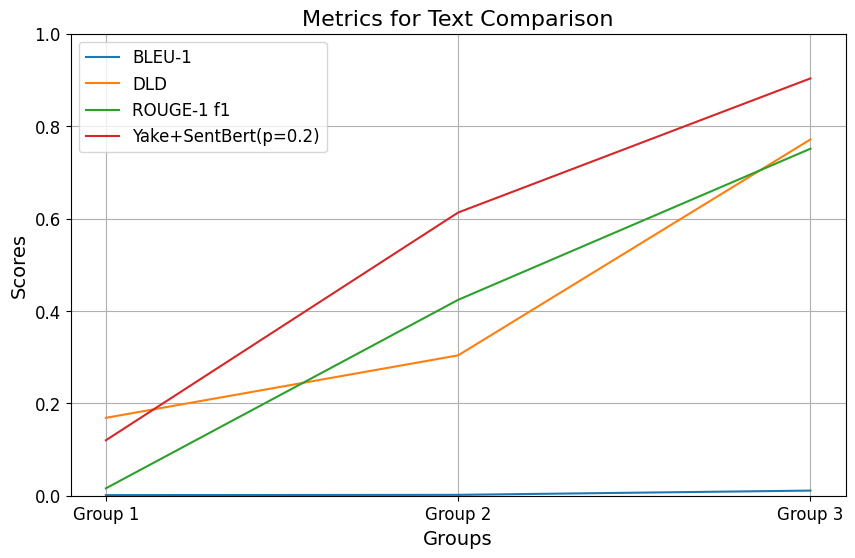
\includegraphics[width=0.45\textwidth]{figures/line-graph.png}
%     \caption{Metric for Text Comparison}
%     \label{fig:textcompare}
%     \vspace{-0.5cm}
% \end{figure}

% Analysis of the plot reveals certain transitional metrics display an upward trend while failing to furnish a fair assessment. The ideal metric yields low scores for group one pair comparisons and high scores for group three pairs. As Figure \ref{fig:textcompare} displays, although exhibiting increased scores from group one to group three, DLD and ROUGE do not account for the robust correlations among text pairs in group three.

% % From analyzing the plot, it is clear that some of the transitional metrics exhibit an upward trend, yet they do not provide a just assessment score. Ideally, we require a metric that yields a low score when comparing group one pairs and a high score when comparing group three pairs. The plot displays in figure \ref{fig:textcompare} reveals that DLD and ROUGE, despite their increasing scores from group 1 to group 3, fail to account for the high correlations among text pairs in group 3. 

% \textit{Ultimately, from the results, it indicates our proposed text comparison metric proves more effective in assessing texts for consistency in this non-emergency dispatching scenario.}

% % The objective is to demonstrate the effectiveness of the text comparison method we propose. We ask dispatchers to (1) evaluate the consistency among a list of texts in a real-world dispatching task, (2) compare our metric with their score, and (3) ask them if the scores make more sense.


\subsection{Confidence-guided Information Itemization}

This experimental setup assesses the performance of the information itemization module of Auto311 using various backends (DistilBERT, BERT, RoBERTa, LongFormer, BigBird \cite{sanh2019distilbert, beltagy2020longformer, zaheer2020big}) and benchmarks (SQuAD, CUAD, TriviaQA \cite{rajpurkar2016squad, rajpurkar2018know, hendrycks2021cuad, joshi2017triviaqa}) and compares it to large language models (LLMs) like GPT3.5 and 4\footnote{Prompt: ``\textit{I will provide context and a set of questions. Please respond to the questions using exact quotes from the context. Your answers should be concise and comprehensive. Context: ...; Question Set: ...''}}, with results in Table \ref{tab:informationextraction}. We utilize our consistency score in this evaluation. Two types of data samples are evaluated for performance: random test samples from archived data (collected by the end of 2022) and the latest data samples (collected from the beginning of 2023) from the call center. Recognizing that city-related information evolves (e.g., new places, activities), we simulate Auto311's usage under knowledge evolution by assessing performance on the latest data samples. Furthermore, we assess Auto311's performance in information itemization when queried with various fields, encompassing basic fields, less specific fields, and more specific fields. Basic fields include essential data like incident location, less specific fields cover descriptors like vehicle and human/suspect descriptions, and more specific fields pertain to incident-specific details such as the timing of the incident (DamagedProperty-when).

% This experimental setup assesses the performance of the information itemization module. We evaluate Auto311's performance in information itemization across various backends (DistilBERT, BERT, RoBERTa, LongFormer, BigBird \cite{sanh2019distilbert, beltagy2020longformer, zaheer2020big}) pre-trained on benchmark datasets (SQuAD, CUAD, TriviaQA \cite{rajpurkar2016squad, rajpurkar2018know, hendrycks2021cuad, joshi2017triviaqa}). Additionally, we compare it with large language models (LLMs) such as GPT3.5 and GPT4 variants\footnote{Prompt: ``\textit{I will provide context and a set of questions. Please respond to the questions using exact quotes from the context. Your answers should be concise and comprehensive.''}}, see results in Table \ref{tab:informationextraction}. We utilize our consistency score in this evaluation. Two types of data samples are evaluated for performance: randomly selected test samples from archived data (collected by the end of 2022) and the latest available data samples (collected from the beginning of 2023) from the local call center. Recognizing that city-related information evolves over time (e.g., new places, activities), we simulate Auto311's usage under knowledge evolution by assessing performance on the latest data samples. Furthermore, we assess Auto311's performance in information itemization when queried with various fields, encompassing basic fields, less specific fields, and more specific fields. Basic fields encompass essential information collected in every call, such as the incident's location (Incident-Location). Less specific fields include descriptors like vehicle description (common in car-related incidents), human/suspect description (relevant in drug-related or welfare check cases), and property description (pertinent to lost-stolen, damaged, or found property cases). More specific fields involve incident-type-specific details, encompassing narrative fields and binary fields like DamagedProperty-when, which inquires about the incident's timing.

% In this experiment setup, we aim to evaluate the performance of the information itemization module. We evaluate Auto311's performance on information itemization with various backends (DistilBERT, BERT, RoBERTa, LongFormer, BigBird \cite{sanh2019distilbert, beltagy2020longformer, zaheer2020big}) pretrained on benchmark datasets (SQuAD, CUAD, TriviaQA \cite{rajpurkar2016squad, rajpurkar2018know, hendrycks2021cuad, joshi2017triviaqa}. We also compare to large language models (LLMs) like ChatGPT variants GPT3.5 and GPT4. Table \ref{tab:informationextraction} shows results. LLMs are constrained to quote words from caller utterances to mimic the extractive process. Our consistency score metric was applied in this evaluation, with two data sample types assessing performance: randomly selected test samples from archived data (collected by the end of 2022) and the latest available data samples (collected from the beginning of 2023) from the local call center. Considering city-related knowledge keeps evolving over time, like newly built places and organized activities, we emulate the usage of Auto311 under knowledge evolution during runtime by also evaluating the performance on the latest data samples. Second, we evaluate Auto311's performance on information itemization when queried with different fields, covering basic fields, less specific fields, and more specific fields. Basic fields include must-collect information in every call, like the location of the incident (Incident-Location). Less specific fields contain fields like vehicle description (likely to appear in most car-related incidents), human/suspect description (likely to appear in drug-pros or check welfare cases), and property description (likely appear in lost-stolen, damaged, or found property cases). More specific fields consist of incident-type-specific fields covering both narrative fields and binary fields like DamagedProperty-when, querying when this incident happened.


% In this experiment setup, we aim to evaluate the performance of the information itemization module. We first evaluate Auto311's performance on information itemization with various backend models (DistilBERT, BERT, RoBERTa \cite{liu2019roberta}, LongFormer \cite{beltagy2020longformer}, BigBird \cite{zaheer2020big}) pretrained on benchmark datasets like SQuAD \cite{rajpurkar2016squad, rajpurkar2018know}, CUAD \cite{hendrycks2021cuad}, TriviaQA \cite{joshi2017triviaqa}. And we also compare its performance with SOTA LLMs (ChatGPT with GPT3.5 \cite{openai_chatgpt_2022}, ChatGPT with GPT4 \cite{openai_gpt4_2023}). The results of this experiment can be found in table \ref{tab:informationextraction}. When comparing with large language models (LLMs), we mandate the provision of answers by quoting callers' exact words. Our consistency score metric was applied in this evaluation, with two data sample types assessing performance: randomly selected test samples from archived data and the latest available data samples from the local call center. The first archived data samples contain previous audio recordings mainly collected by the end of 2022, which Auto311 is trained on. The second latest samples are collected mainly from the beginning of 2023. Considering city-related knowledge keeps evolving over time, we find the latest samples cover time-sensitive information like newly built places and organized activities. Thus, we further emulate the usage of Auto311 under knowledge evolution during runtime. 



% In the competition with LLMs, we have required them to provide answers by quoting the exact words spoken by the caller. Our consistency score metric has been used in this evaluation, and we have used three types of data samples to assess performance. These include test samples randomly selected from the entire dataset, new samples provided by DEC from the latest phone calls, and synthesized samples based on previous question-answer pairs. Batch 3 has been synthesized using a data enrichment algorithm similar to the one used in \cite{chen2022cityspec, chen2023cityspec}.  In addition to batch-wise evaluation, we also test the performance of our module on different question types including unseen specific questions under one certain incident type, e.g., ``what is the color of the vehicle?'' and ``when did this happen?'', see results in Table \ref{tab:different_question_types}.

\begin{table}[h]
\centering
\caption{Performance on information itemization}
\scriptsize
\begin{tabular}{||c|c|c||}
\hline
           & Archived Samples (test) & Latest Samples (runtime)  \\ \hline\hline
DistilBERT-SQuAD2 &  0.5546    & 0.5330                        \\ \hline        
BERT-SQuAD2 &   0.2422   & 0.2791                        \\ \hline
RoBERTa-SQuAD2 &   0.1172   & 0.2581                        \\ \hline
RoBERTa-CUAD &   0.2188   & 0.2378                        \\ \hline
LongFormer-TriviaQA &   0.3260   & 0.1424                        \\ \hline
BigBird-TriviaQA &   0.5289   &     0.5015                    \\ \hline
GPT3.5 (June 2023)     &   0.6343   & 0.6529                         \\ \hline
GPT4 (June 2023)      &   0.6578   & 0.6264                          \\ \hline
\textbf{Auto311}   &   \textbf{0.9329}   & \textbf{0.8605}          \\ \hline
\end{tabular}
\label{tab:informationextraction}
\end{table}

\begin{table*}[t]
\centering
\caption{Auo311's performance on different fields}
\scriptsize
\begin{tabular}{||c|ccccccccc||}
\hline
                  & \multicolumn{3}{c|}{Basic Fields}                                                                                                                                                                                                                                                                                           & \multicolumn{6}{c||}{Less Specific Feilds}                                                                                                                                                                                  \\ \hline\hline
                  & \multicolumn{1}{c|}{Incident-Location}                                                                & \multicolumn{1}{c|}{Caller-Name}                                                                           & \multicolumn{1}{c|}{Caller-Phone \#}                                                                   & \multicolumn{2}{c|}{Vehicle Description}                                       & \multicolumn{2}{c|}{Human/Suspect Description}                                 & \multicolumn{2}{c||}{Property Descritpion}                \\ \hline
w/o Conf Guide    & \multicolumn{1}{c|}{0.9035}                                                                           & \multicolumn{1}{c|}{0.9478}                                                                                & \multicolumn{1}{c|}{1.0000}                                                                            & \multicolumn{2}{c|}{0.8538}                                                    & \multicolumn{2}{c|}{0.9678}                                                    & \multicolumn{2}{c||}{0.9512}                              \\ \hline
w/ Conf Guide     & \multicolumn{1}{c|}{\textbf{0.9631}}                                                                  & \multicolumn{1}{c|}{\textbf{0.9962}}                                                                       & \multicolumn{1}{c|}{\textbf{1.0000}}                                                                   & \multicolumn{2}{c|}{\textbf{0.9104}}                                           & \multicolumn{2}{c|}{\textbf{1.0000}}                                           & \multicolumn{2}{c||}{\textbf{1.0000}}                     \\ \hline\hline
                  & \multicolumn{9}{c|}{More Specific Fields}                                                                                                                                                                                                                                                                                                                                                                                                                                                                                                                \\ \hline\hline
\multirow{2}{*}{} & \multicolumn{1}{c|}{\multirow{2}{*}{\begin{tabular}[c]{@{}c@{}}DamagedProperty\\ -When\end{tabular}}} & \multicolumn{1}{c|}{\multirow{2}{*}{\begin{tabular}[c]{@{}c@{}}AggressiveDriver\\ -Behavior\end{tabular}}} & \multicolumn{1}{c|}{\multirow{2}{*}{\begin{tabular}[c]{@{}c@{}}CheckWelfare\\ -Relation\end{tabular}}} & \multicolumn{3}{c|}{\begin{tabular}[c]{@{}c@{}}MinorCrash\\ -BlockTraffic (Y/N)\end{tabular}}                          & \multicolumn{3}{c||}{\begin{tabular}[c]{@{}c@{}}CheckWelfare\\ -InpersonMeet (Y/N)\end{tabular}}   \\ \cline{5-10} 
                  & \multicolumn{1}{c|}{}                                                                                 & \multicolumn{1}{c|}{}                                                                                      & \multicolumn{1}{c|}{}                                                                                  & \multicolumn{1}{c|}{P}                 & \multicolumn{1}{c|}{R}                & \multicolumn{1}{c|}{F-1}              & \multicolumn{1}{c|}{P}                 & \multicolumn{1}{c|}{R}                & F-1              \\ \hline
w/o Conf Guide    & \multicolumn{1}{c|}{0.9045}                                                                           & \multicolumn{1}{c|}{0.8255}                                                                                & \multicolumn{1}{c|}{0.9023}                                                                            & \multicolumn{1}{c|}{66.67\%}          & \multicolumn{1}{c|}{100.00\%}          & \multicolumn{1}{c|}{80.0\%}           & \multicolumn{1}{c|}{83.33\%}           & \multicolumn{1}{c|}{83.33\%}          & 83.33\%          \\ \hline
w/ Conf Guide     & \multicolumn{1}{c|}{\textbf{1.000}}                                                                   & \multicolumn{1}{c|}{\textbf{0.9164}}                                                                       & \multicolumn{1}{c|}{\textbf{0.9855}}                                                                   & \multicolumn{1}{c|}{\textbf{88.89\%}} & \multicolumn{1}{c|}{\textbf{100.00\%}} & \multicolumn{1}{c|}{\textbf{94.12\%}} & \multicolumn{1}{c|}{\textbf{83.33\%}} & \multicolumn{1}{c|}{\textbf{100.00\%}} & \textbf{90.91\%} \\ \hline
\end{tabular}
\label{tab:confidence_on_different_question_types}
\end{table*}


% \begin{table}[h]
% \centering
% \caption{Performance of the information extracting module}
% \scriptsize
% \begin{tabular}{||c|c|c|c||}
% \hline
%            & Test Batch & Latest Batch & Synthesized (Nashville) \\ \hline\hline
% DistilBERT-SQuAD &  0.5546    & 0.5330     &    0.7553                     \\ \hline        
% DistilBERT-adapted &   0.9329   & 0.8605     & 0.9849                       \\ \hline
% BERT-SQuAD &   0.2422   & 0.2791     &     0.8136                    \\ \hline
% BERT-adapted   &   0.7907   &      0.7244      &   0.9457                      \\ \hline
% GPT3.5     &   0.6343   & 0.6529     &    0.9078                     \\ \hline
% GPT4       &   0.6578   & 0.6264     &   0.9794                      \\ \hline
% Claude 2   &   0.8113   & 0.8850     &   0.9545                      \\ \hline
% \end{tabular}
% \label{tab:informationextraction}
% \end{table}

Table \ref{tab:informationextraction} yields the following insights: (1) pretrained model limitations: DistilBERT and BERT struggle in current non-emergency dispatch scenarios, performing notably lower than other methods. For instance, BERT pretrained on SQuAD achieves only 0.2422 on the test batch; (2) LLMs vs. Auto311: Despite LLMs' general NLP success, Auto311 consistently outperforms them on both datasets. For example, Auto311's performance surpasses GPT3.5 by 47\% on archived samples and 41\% on the latest samples; (3) adaptation to evolving knowledge: Auto311's 37\% performance lead over GPT4, despite a minor drop, underscores its proficiency in capturing evolving local city knowledge.

% From Table \ref{tab:informationextraction}, we make the following observations. 
% First, despite high performance on datasets such as SQuAD, existing pretrained models including DistilBERT and BERT fail to handle current non-emergency dispatch scenarios, with scores noticeably lower than other approaches. For example, the BERT model pertained on SQuAD only obtains 0.2422 on the test batch.
% Second, although LLMs like GPT achieve great success on general-purpose NLP tasks, they still do not entirely outperform Auto311 on both datasets. For example, Auto311 outperforms GPT3.5 by 47\% on archived samples and 41\% on latest samples.
% Third, although the performance drops by 0.0724, we find Auto311 still outperforms LLMs, 37\% higher than GPT4, by decently capturing the evolving knowledge in the local city.

Table \ref{tab:confidence_on_different_question_types} highlights how confidence guidance enhances itemization across field types, e.g., improving consistency from 0.8255 to 0.9164 for aggressive driver behavior details. Auto311 achieves 100\% recall for binary questions, correctly predicting traffic blockage and in-person meetup needs. In real-world non-emergency scenarios, prioritizing high recall ensures comprehensive coverage of potential requests. Results showcase confidence scoring's role in optimizing itemization, particularly for critical binary fields.

% Table \ref{tab:confidence_on_different_question_types} shows confidence guidance improves itemization across field types, e.g. increasing consistency from 0.8255 to 0.9164 for aggressive driver behavior details. For binary questions, Auto311 achieves 100\% recall for both fields, which means it correctly predicts all utterances implying traffic blockage and in-person meetup needs.  In real-world scenarios like non-emergency call handling, we prioritize a higher recall rate, since it guarantees all potential requests are met. Results demonstrate confidence scoring enhances itemization, with optimized recall for critical binary fields.

% From Table \ref{tab:confidence_on_different_question_types}, we find that with the introduction of confidence guidance, Auto311's performance on information itemization in different fields is further improved, e.g., with a consistency score increased from 0.8255 to 0.9164 when fulfilling fields specifically requesting what is the behavior of the aggressive driver. In the last two binary questions, Auto311 achieves a 100.00\% recall score. In real-world scenarios like non-emergency call handling, we prioritize a higher recall rate, since it guarantees all potential requests are met. Thus, the 100\% recall rate indicates that all the caller utterances implying the traffic is blocked or an in-person meetup is needed are predicted correctly.

\textit{In summary, the results underscore the difficulty of the information itemization task for both pretrained models and existing LLMs. Auto311's fine-tuning on our dataset effectively integrates task-specific knowledge, leading to competitive performance surpassing LLMs. Moreover, through runtime emulation, Auto311 adapts to evolving city knowledge, indicating potential for long-term deployment. Additionally, confidence guidance empowers Auto311 to enhance the completion of various case report fields.}

% \textit{In summary, this table indicates, the information itemization task challenges both pretrained models and available LLMs. With fine-tuning on our dataset, this task-specific knowledge is successfully injected into Auto311, yielding competitive performance exceeding LLMs. Additionally, based on runtime emulation, Auto311 is also able to capture the evolving city knowledge, showing potential in a long-time deployment. Furthermore, the confidence guidance grants Auto311 improvements in fulfilling different fields on the case report.}

% First, although existing pretrained models like DistilBERT and BERT yield high performance on datasets like SQuAD, those models fail to deal with current non-emergency dispatching scenarios, and their scores are obviously lower than other approaches. E.g., the BERT model pretrained on SQuAD only obtains 0.2422 on the test batch. 
% Second, after fine-tuning pretrained models on our dataset, both DistilBERT and BERT achieve competitive performances when compared to SOTA LLMs in most cases, e.g., DistilBERT archives a score of 0.9329 on the test batch, higher than all other backend models, and it outperforms all other backend models trying to answer the initial 6 questions types.
% % We also notice that Claude 2 outperforms DistilBERT on the latest bath by 0.02, we carefully review the predictions from both models and find this small gap is caused by our limited training set.
% Last, fine-tuned models still perform well on synthesized inputs with unseen city-specific features or even entirely unseen inputs. E.g., fine-tuned DistilBERT scores 0.9849 on the synthesized batch and 0.9322 on more specific questions that did not even appear during the training phase.  

% \textit{In summary, both tables indicate, no matter whether batch-wise or question-type-wise, fine-tuning pretrained models can effectively inject task-specific knowledge into our module and result in a better overall performance even when compared to SOTA LLMs under the current scenario.}

% Question-answering model performance: the objective is to demonstrate the efficacy of the DistilBERT QA system and establish the necessity of fine-tuning. This will be achieved through (1) analyzing the performance (in terms of our proposed metric) of DistilBERT prior to being fine-tuned on our dataset and (2) testing the various back-end models, including BERT and its variants.
% \subsection{Potential Cross-City Deployment}
% We also evaluate the information itemization module's performance alongside state-of-the-art LLMs for potential cross-city deployment to demonstrate transfer learning potential and future adaptability to diverse scenarios. Specifically, case studies utilize New York City, Washington DC, Los Angeles, and Atlanta. Caller context synthesis leverages a similar data enrichment algorithm as previous experiments along with city-level features from \cite{chen2022cityspec, chen2023cityspec}.

% We also test our module performance along with SOTA LLMs in possible cross-city deployment, to show its potential in transfer learning and future adaptation under different scenarios. Here specifically, we choose New York City, Washington DC, Los Angles, and Atlanta for case studies. We synthesize the caller's context using a similar data enrichment algorithm applied in previous experiments and city-level features from \cite{chen2022cityspec, chen2023cityspec}. 

% \begin{table}[H]
% \centering
% \caption{Performance of the information extracting module in unseen scenarios}
% \scriptsize
% \begin{tabular}{||c|c|c|c|c||}
% \hline
%            & NYC, NY & WAS, DC & LA, CA & ATL, GA  \\ \hline\hline
% DistilBERT-adapted &   \textbf{0.9976}  &  \textbf{0.9892}  &  \textbf{0.9933}  &   \textbf{0.9989}   \\ \hline
% BERT-adapted       &  0.9418   &  0.9802  &  0.964  &  0.9614     \\ \hline
% GPT3.5     &  0.9304   &  0.9215  &  0.8736  & 0.9202   \\ \hline
% GPT4       &  0.9917   &  0.9876  &  0.9905  &  0.9893 \\ \hline
% Claude 2   &  0.9423   &  0.9413  &  0.9474  &  0.9464  \\ \hline
% \end{tabular}
% \end{table}

% \textit{In summary, although our system never learns the city-featured vocabulary from unseen cities, it still performs close to (statistically higher than) SOTA LLMs in terms of our consistency score. This promising performance indicates there can be potential cross-city deployment opportunities for our system.}

\subsection{System Level Performance}


The subsequent experiments focus on assessing Auto311's system-level performance. Due to data limitations, audio recordings only capture fixed dialogue paths, preventing direct interaction with the same caller in identical call scenarios. Instead, we emulate conversations by merging utterance segments. This emulation facilitates evaluating Auto311's capabilities in two aspects: (1) assessing its management of changing incident types and (2) analyzing the optimization of follow-up dialogues during emulation.

% The following experiments focus on evaluating Auto311's system-level performance. Due to the data characteristics, audio recordings only capture fixed dialogue trajectories, which further means Auto311 cannot directly interact with the same caller under the same call scenario. Instead, we emulate conversations by combining utterance segments. Emulated conversations allow assessing Auto311 on the following two abilities: (1) analyzing Auto311's handling of shifting incident types, and (2) analyzing Auto311's follow-up dialogue optimization under emulation. 
 

% The following experiments focus on evaluating Auto311's system-level performance. Due to the data characteristics, audio recordings only capture fixed dialogue trajectories, which further means Auto311 cannot directly interact with the same caller under the same call scenario. Thus, to comprehensively evaluate Auto311 at a system level, we emulate the conversation by combining previous caller utterance segments. This section includes two different experiments: (1) analyzing how Auto311 handles shifting incident types during the call, and (2) analyzing how well can Auto311 utilize given information to optimize follow-up dialogues as a system under emulation.

% \subsubsection{Influences on Incident Type Prediction}
% We first test the influences brought by the confidence guidance on the incident type prediction module independently. In Table \ref{tab:confidence_on_different_incident_types}, we record the performance improvements with confidence guidance kept active during running. Based on the experimental results, we make the following observation: although pretraining BERT on our dataset has already granted the incident type module a satisfying ability to predict all the possible incident types given a call utterance, with confidence guidance, the module is still improved by rejecting outputs with lower confidence scores.

% \begin{table*}[t]
% \centering
% \caption{Performance of the information extracting module regarding different questions}
% \scriptsize
% \begin{tabular}{||c|cccc|cccc|cccc||}
% \hline
% Incident Type & \multicolumn{4}{c|}{Minor Crash Report}                                                            & \multicolumn{4}{c|}{Lost or Stolen Property}                                                       & \multicolumn{4}{c||}{Aggressive Drivers}                                                            \\ \hline\hline
% Metric        & \multicolumn{1}{c|}{Precision} & \multicolumn{1}{c|}{Recall} & \multicolumn{1}{c|}{F-1} & Accuracy & \multicolumn{1}{c|}{Precision} & \multicolumn{1}{c|}{Recall} & \multicolumn{1}{c|}{F-1} & Accuracy & \multicolumn{1}{c|}{Precision} & \multicolumn{1}{c|}{Recall} & \multicolumn{1}{c|}{F-1} & Accuracy \\ \hline
% Bert-unguided & \multicolumn{1}{c|}{93.06\%}          & \multicolumn{1}{c|}{97.10\%}       & \multicolumn{1}{c|}{95.04\%}    &     95.76\%     & \multicolumn{1}{c|}{88.00\%}          & \multicolumn{1}{c|}{95.65\%}       & \multicolumn{1}{c|}{91.67\%}    &     95.60\%     & \multicolumn{1}{c|}{93.75\%}          & \multicolumn{1}{c|}{90.91\%}       & \multicolumn{1}{c|}{92.31\%}    &     93.75\%     \\ \hline
% Bert-guided   & \multicolumn{1}{c|}{\textbf{97.10\%}}          & \multicolumn{1}{c|}{\textbf{94.37\%}}       & \multicolumn{1}{c|}{\textbf{95.71\%}}    &     \textbf{96.34\%}     & \multicolumn{1}{c|}{\textbf{90.91\%}}          & \multicolumn{1}{c|}{95.20\%}       & \multicolumn{1}{c|}{\textbf{93.00\%}}    &    \textbf{96.70\%}      & \multicolumn{1}{c|}{93.75\%}          & \multicolumn{1}{c|}{\textbf{93.75\%}}       & \multicolumn{1}{c|}{\textbf{93.75\%}}    &    \textbf{94.94\%}      \\ \hline\hline
% Incident Type & \multicolumn{4}{c|}{Check Welfare}                                                                 & \multicolumn{4}{c|}{Damaged Property}                                                              & \multicolumn{4}{c||}{Noise Violation}                                                               \\ \hline\hline
% Metric        & \multicolumn{1}{c|}{Precision} & \multicolumn{1}{c|}{Recall} & \multicolumn{1}{c|}{F-1} & Accuracy & \multicolumn{1}{c|}{Precision} & \multicolumn{1}{c|}{Recall} & \multicolumn{1}{c|}{F-1} & Accuracy & \multicolumn{1}{c|}{Precision} & \multicolumn{1}{c|}{Recall} & \multicolumn{1}{c|}{F-1} & Accuracy \\ \hline
% Bert-unguided & \multicolumn{1}{c|}{93.10\%}          & \multicolumn{1}{c|}{87.10\%}       & \multicolumn{1}{c|}{90.00\%}    &     90.63\%     & \multicolumn{1}{c|}{80.00\%}          & \multicolumn{1}{c|}{100.00\%}       & \multicolumn{1}{c|}{88.89\%}    &     94.12\%     & \multicolumn{1}{c|}{100.00\%}          & \multicolumn{1}{c|}{71.43\%}       & \multicolumn{1}{c|}{83.33\%}    &    93.75\%      \\ \hline
% Bert-guided   & \multicolumn{1}{c|}{93.10\%}          & \multicolumn{1}{c|}{87.10\%}       & \multicolumn{1}{c|}{90.00\%}    &     90.63\%     & \multicolumn{1}{c|}{\textbf{88.89\%}}          & \multicolumn{1}{c|}{100.00\%}       & \multicolumn{1}{c|}{\textbf{94.12\%}}    &     \textbf{96.88\% }    & \multicolumn{1}{c|}{100.00\%}          & \multicolumn{1}{c|}{71.43\%}       & \multicolumn{1}{c|}{83.33\%}    &      93.75\%    \\ \hline\hline
% Incident Type & \multicolumn{4}{c|}{Roadway Hazard}                                                                & \multicolumn{4}{c|}{Abandoned Vehicles}                                                            & \multicolumn{4}{c||}{Drug or Prostitution Activity}                                                 \\ \hline\hline
% Metric        & \multicolumn{1}{c|}{Precision} & \multicolumn{1}{c|}{Recall} & \multicolumn{1}{c|}{F-1} & Accuracy & \multicolumn{1}{c|}{Precision} & \multicolumn{1}{c|}{Recall} & \multicolumn{1}{c|}{F-1} & Accuracy & \multicolumn{1}{c|}{Precision} & \multicolumn{1}{c|}{Recall} & \multicolumn{1}{c|}{F-1} & Accuracy \\ \hline
% Bert-unguided & \multicolumn{1}{c|}{100.00\%}          & \multicolumn{1}{c|}{83.33\%}       & \multicolumn{1}{c|}{90.91\%}    &     93.10\%     & \multicolumn{1}{c|}{100.00\%}          & \multicolumn{1}{c|}{88.89\%}       & \multicolumn{1}{c|}{94.12\%}    &    95.00\%      & \multicolumn{1}{c|}{85.17\%}          & \multicolumn{1}{c|}{100.00\%}       & \multicolumn{1}{c|}{92.40\%}    &     92.86\%     \\ \hline
% Bert-guided   & \multicolumn{1}{c|}{100.00\%}          & \multicolumn{1}{c|}{83.33\%}       & \multicolumn{1}{c|}{90.91\%}    &     93.10\%     & \multicolumn{1}{c|}{100.00\%}          & \multicolumn{1}{c|}{88.89\%}       & \multicolumn{1}{c|}{94.12\%}    &     95.00\%     & \multicolumn{1}{c|}{85.17\%}          & \multicolumn{1}{c|}{100.00\%}       & \multicolumn{1}{c|}{92.40\%}    &     92.86\%     \\ \hline
% \end{tabular}
% \label{tab:confidence_on_different_incident_types}
% \end{table*}

% \subsubsection{Influences on Information Itemization}
% Similarly, we also test the influences brought by the confidence guidance on the information itemization module. In Table \ref{tab:confidence_on_different_question_types}, we record the performance improvements with confidence guidance kept active during running.


\subsubsection{Adjustments to Shifting Incident Types}

We evaluate Auto311's adaptability to shifting incident types. Using common shifts observed in the dataset (see Figure \ref{fig:conf_curve}), we emulate conversations where the caller firmly states type A (blue lines and grey regions), then adds type-specific details for type B (orange lines and regions), indicating a type shift. These experiments assess Auto311's real-time adaptation to emergent types in emulated interactions.

% As discussed, the ongoing calls could involve multiple types. We evaluate Auto311's ability to adjust to shifting types. Experiments use common shifts observed from the dataset (see Figure \ref{fig:conf_curve}): minor crash to aggressive driver (subplot a), minor crash to road hazard (subplot b), damaged property to lost/stolen (subplot c), noise violation to check welfare (subplot d). Conversations are emulated by the caller first firmly stating type A (marked with blue lines and grey regions), then adding more type-specific details for type B (marked with orange lines and orange regions), indicating a type shift. Experiments assess end-to-end adaptation to emergent types in emulated interactions.

% Previous sections evaluated static prediction - here we analyze handling type shifts dynamically with accumulating utterances and confidence guidance.

% As discussed in Section Motivating Study, there are approximately 38.27\% percent of recordings involving more than one incident type. In this experiment, we evaluate and analyze Auto311's ability to adjust to the shifting incident types during the conversation, which further enables it to dynamically generate case reports. To fully evaluate Auto311's ability to handle multiple incident types, we select the most popular shifting situations from the dataset, see Figure \ref{fig:conf_curve}: from minor crash report to aggressive driver (subplot a), from minor crash report to roadway hazard (subplot b), from damaged property to lost stolen property (subplot c), and from noise violation to check welfare (subplot d). In emulation, we compose the conversations by first firmly reporting the ongoing incident type is A (marked with blue lines and grey regions), then continuously supplementing specific details under type B (marked with orange lines and orange regions). Note, the previous discussion only covers Auto311's performance on incident type prediction with a static caller utterance provided. However, in this section, we analyze and discuss Auto311's ability to shift from one incident type to another with more and more utterances being collected dynamically with confidence guidance.

\begin{figure}[h]
    \centering
    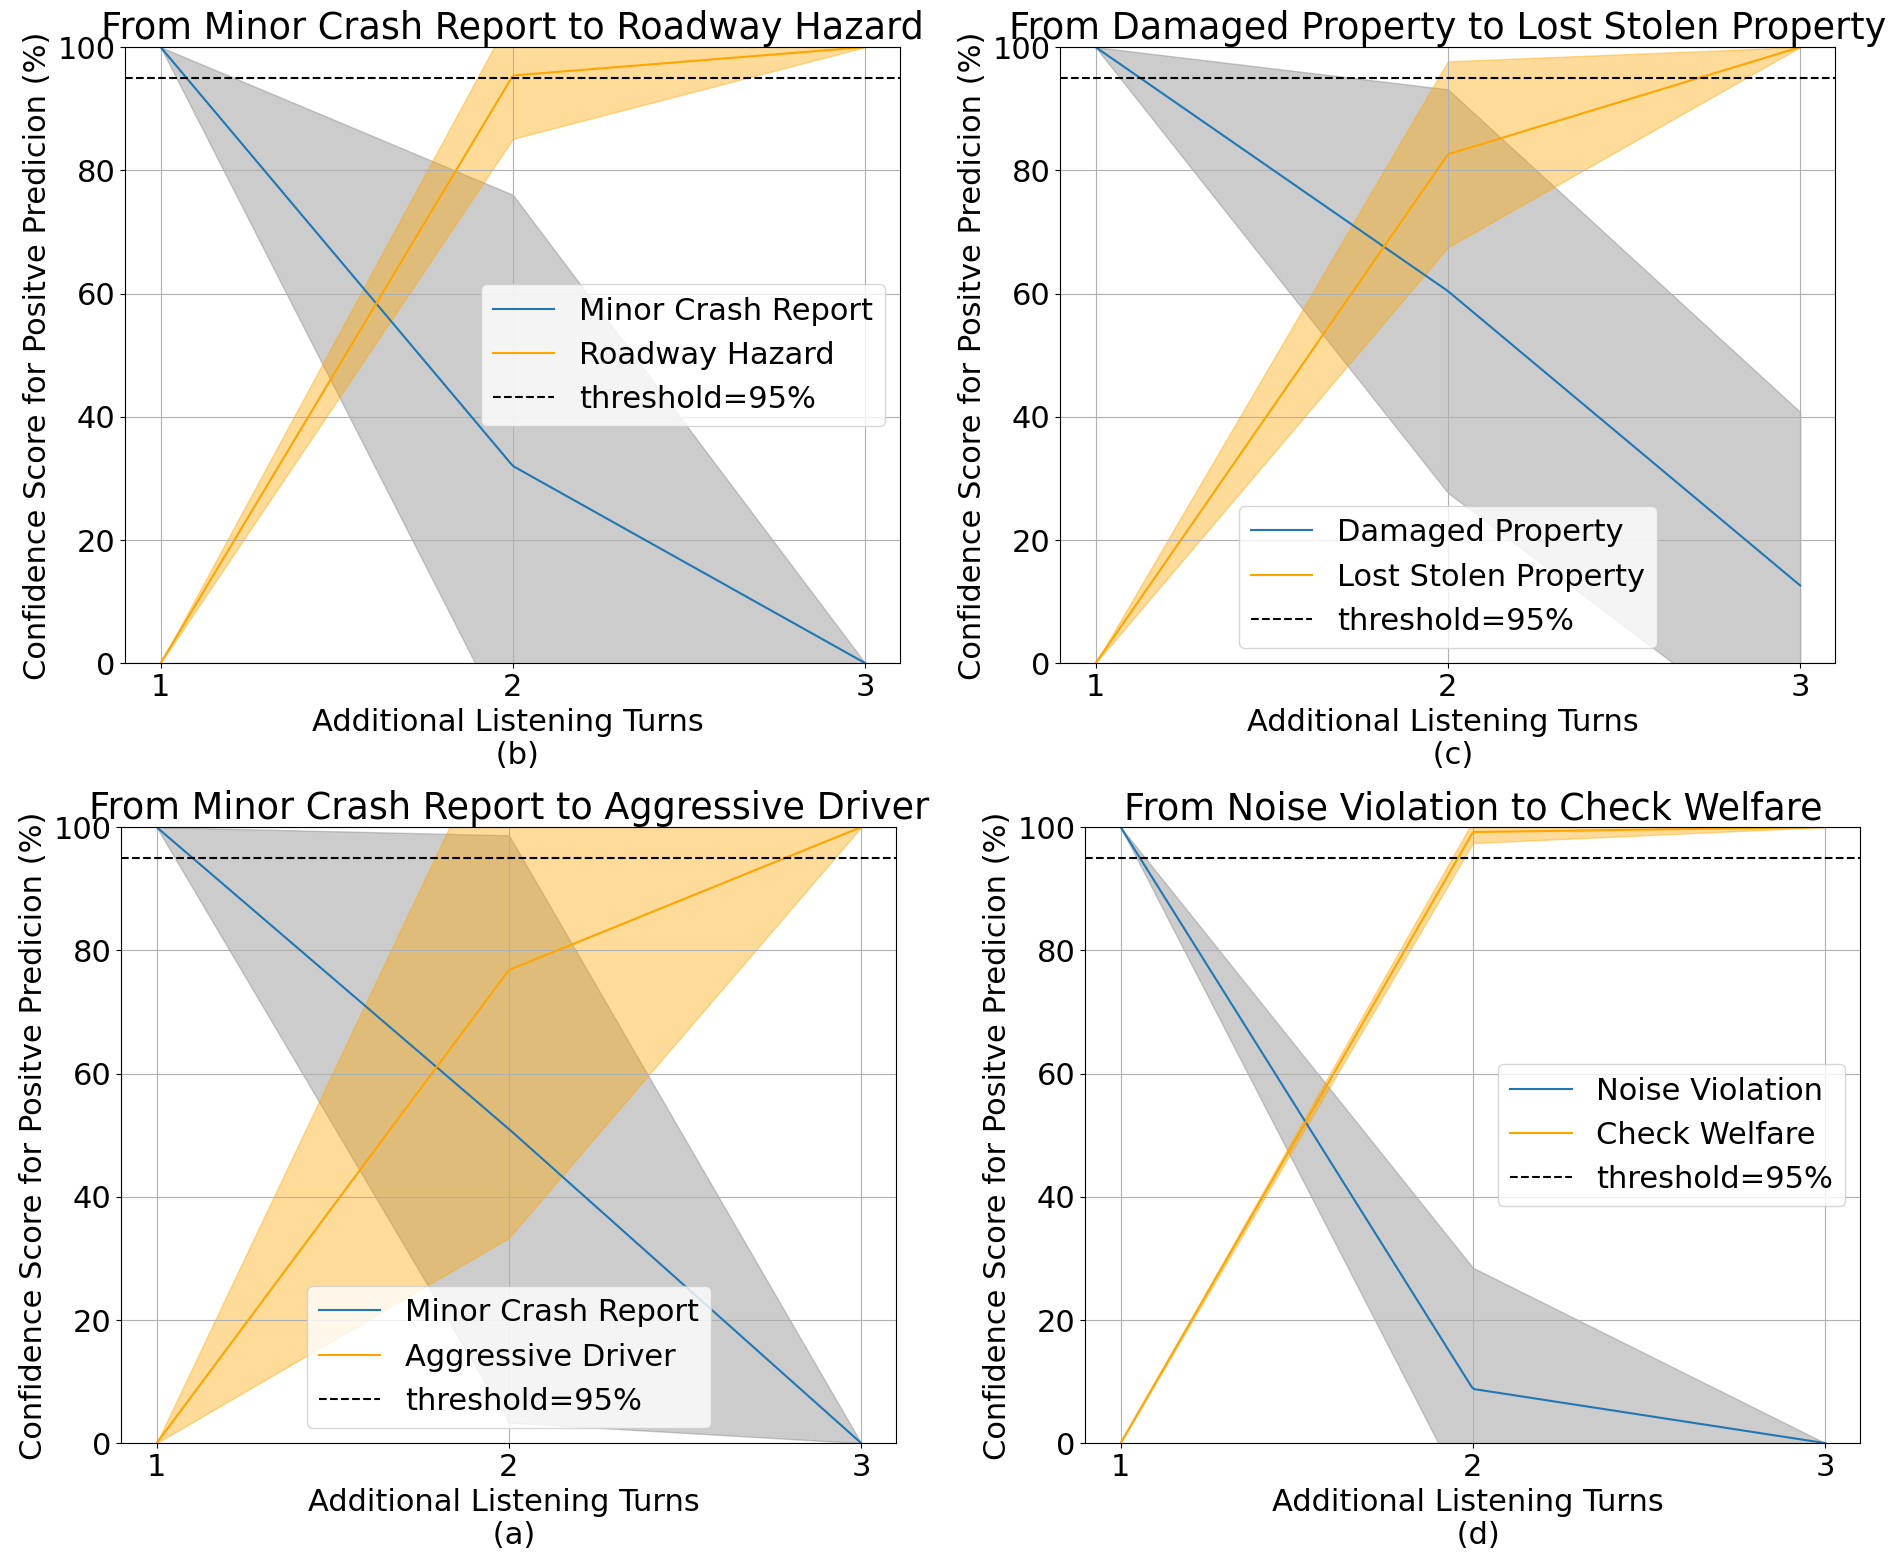
\includegraphics[width=0.40\textwidth]{figures/conf_curve.png}
    \caption{Confidence Changes in Shifting Incident Types}
    \label{fig:conf_curve}
    \vspace{-0.5cm}
\end{figure}

From Figure \ref{fig:conf_curve}, we observe that first, Auto311 handles all four major shifting situations in three future turns with more type-specific descriptions being fed as input to the incident type prediction module. Second, with the introduction of confidence guidance, Auto311 adjusts the prediction results to align with the shifting trend dynamically.

\textit{In summary, Auto311 adeptly handles shifting incident types in simulations, updating its understanding and creating optimized reports with more specific information over 3 follow-up turns.}

% \textit{In summary, based on our experimental results, Auto311 is capable of handling multiple incident types not only by statically accurately telling all the types but also by appropriately adjusting to shifting incident types with more specific information being fed in few follow-up turns.}

\subsubsection{Optimizations to Upcoming Dialogues}

We emulate Auto311 usage by composing caller utterances and assessing the relationship between saved turns and utterance size (see Figure \ref{fig:emulation}). Utterance size represents the count of past segments included. Across 100 emulations per size, we monitor saved turns and categorization accuracy. These experiments evaluate Auto311's ability to optimize dialogues through accumulated context and to make type predictions effectively.

% We emulate Auto311 usage by feeding composed caller utterances and analyzing turns saved versus utterance size (Figure \ref{fig:emulation}). Utterance size refers to the number of past segments in the composed utterance. Size $n$ means $n$ previous segments are included. In 100 emulations per size, we monitor dialogue turns saved by Auto311 and also the accuracy in categorizing the composed utterances. Experiments assess Auto311's ability to optimize upcoming dialogues by leveraging accumulating context and prediction accuracy.

% To demonstrate Auto311's ability to optimize upcoming dialogues, we emulate the process of the usage of Auto311 by feeding the composed caller utterance to Auto311. During emulation, we analyze the number of turns that can be saved in future conversations with respect to the size of the composed utterances (100 emulations for each size), see Figure \ref{fig:emulation}, and monitor Auto311's accuracy in categorizing the composed utterances. The utterance size refers to the number of utterance segments used in the composed utterance; size $n$ means there are $n$ previous utterance segments included in the composed utterances. 


Longer composed utterances contain more itemizable details. The blue line indicates Auto311's saved turns during emulation, while the light blue region represents total information provided. The average and maximum real-world utterance lengths are denoted by green and red dashed lines. Emulation demonstrates Auto311 effectively using additional information in caller utterances to minimize follow-up turns. Furthermore, Auto311 achieves a 94.49\% accuracy (not shown in Figure \ref{fig:emulation}) when handling composed utterances.

% Larger composed utterances contain more itemizable information. The blue line shows turns saved by Auto311 under emulation. The light blue region indicates the total information provided. Green and red dashed lines show average and maximum real-world utterance lengths. From the emulation, we find Auto311 is able to fully utilize the additional information conveyed in caller utterances to save follow-up turns. Additionally, Auto311 reports an overall accuracy of 94.49\% (not shown in Figure \ref{fig:emulation}) when faced with composed utterances.

% We observe that as the size of composed utterances gets larger, it contains more additional information for Auto311 to itemize. The blue line shows the turns saved by Auto311 under emulation. The light blue region indicates the amount of provided information based on current utterances. Green and red dashed lines indicate the average and maximum length of all the real-world caller utterances correspondingly. From the emulation, we find (1) Auto311 is able to fully utilize the additional information conveyed in caller utterances to save follow-up turns. Additionally, Auto311 reports an overall accuracy of 94.49\% when faced with composed utterances.


\begin{figure}[h]
    \centering
    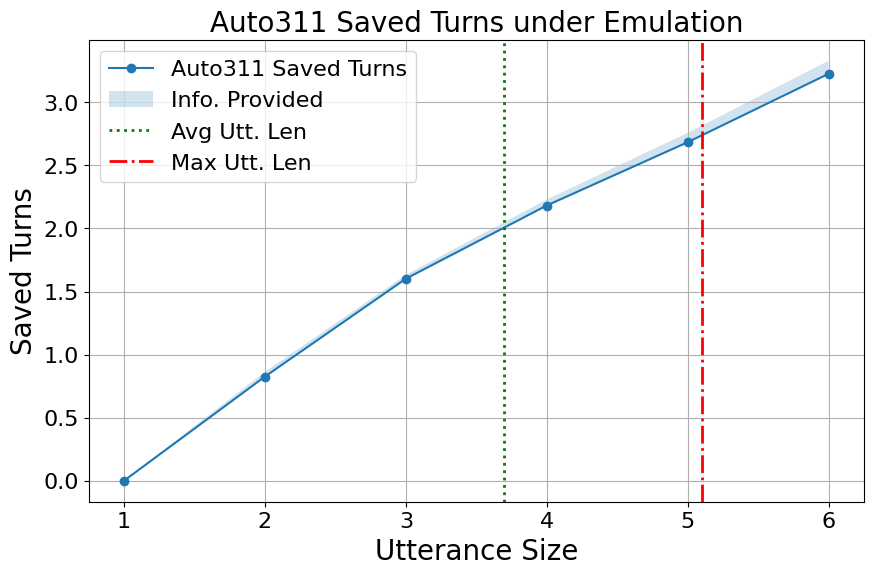
\includegraphics[width=0.40\textwidth]{figures/emulation.png}
    \caption{Emulated Usage of Auto311}
    \label{fig:emulation}
    \vspace{-0.5cm}
\end{figure}





% To demonstrate the impacts of our proposed system in real-world deployment, we simulate the working situation by emulating 10 random batches from the audio recordings to analyze (1) how many interactions can be potentially saved in further conversation based on the first few turns of dialogue and (2) how accurately can our system categorize the ongoing call. After our 10 emulations, with the assistance of our system, an average of 1.01 with a maximum of 1.86 turns can be theoretically reduced in future conversations based on the information provided in real audio recordings. Meanwhile, our system reports an overall accuracy of 94.49\% when dispatching the ongoing call to given incident types.

% \textit{In summary, the emulations demonstrate, at a system level, Auto311: (1) piratically optimizes future dialogues by fully utilizing additional utterance information. (2) effectively categorizes potential incident types with 94.49\% overall accuracy.}

\textit{In summary, these emulations prove our solution, at a system level, not only piratically optimizes future conversations by utilizing additional information provided in caller utterances but also effectively categorizes the potential incident types with an overall accuracy of 94.49\%.}


\section{Related Work}

\textbf{Question Answering and Large Language Models.} In recent years, advanced question-answering systems have evolved across various scenarios \cite{chen2023cityspecshield, chen2022intelligent, chen2022cityspec, diefenbach2018core}. Black-box abstractive QA systems like mBART and T5 \cite{chipman2022mbart, raffel2019t5} lack output control. Although large language models, especially for QA dialogues \cite{brown2020language, ouyang2022training, claude2_2023}, gain attention, we still argue that prompt-based models are unsuitable for emergency response due to compromised input preservation and advocate for a transparent, controllable offline approach prioritizing reliability and decision transparency.

% In recent years, significant efforts have been made to create advanced question-answering systems across various scenarios \cite{allam2012question, hirschman2001natural, diefenbach2018core}. While abstractive QA systems like fine-tuned mBART and T5 \cite{chipman2022mbart, raffel2019t5} are also widely used, they often lack output control as black-box models. Large language models, especially for QA dialogues, are gaining attention \cite{brown2020language, ouyang2022training, claude2_2023}. However, we contend that prompt-based models are unsuitable for emergency response due to their potential to compromise user utterance preservation, which is considered critical for accuracy and reliability in emergency response. Thus, a more transparent and controllable offline approach, prioritizing original input preservation and model decision elucidation, is necessary.



% Recent years have witnessed significant efforts to develop advanced question-answering systems for diverse scenarios \cite{allam2012question, hirschman2001natural, diefenbach2018core}. Abstractive QA systems, including fine-tuned mBART and T5\cite{chipman2022mbart, raffel2019t5}, are often considered text-to-text black-box models with limited output control. Large language models also gain increasing attention, especially for question-answering dialogues \cite{brown2020language, ouyang2022training, claude2_2023}. However, despite advances in prompt-based models, we argue they prove unsuitable for emergency response systems, as they may compromise preserving users’ initial utterances, critical for system accuracy and reliability. Thus, a more transparent, controllable approach prioritizing original input preservation and elucidating model decision-making should be adopted.



% In recent years, significant efforts have been dedicated to the development of advanced question-answering systems under various scenarios \cite{allam2012question, hirschman2001natural, diefenbach2018core}. Among them, abstractive question-answering (QA) systems, such as fine-tuned mBART \cite{chipman2022mbart}, are often considered as text2text black-box generation models, with limited control over the output. Large language models (LLMs) are also drawing more and more attention in Natural Language Processing applications, especially when the interactions are carried out in a question-answering dialogue \cite{brown2020language, ouyang2022training, claude2_2023}. Despite recent huge advancements in prompt-based language models, we argue that these methods are unsuitable for the current task of emergency response systems, as they may jeopardize the preservation of the initial user utterance, which is paramount for ensuring the accuracy and reliability of the system. Therefore, a more transparent and controllable approach should be adopted, which prioritizes the preservation of the user's initial input and provides a clearer understanding of the model's decision-making process.

\noindent\textbf{Confidence Scores in Machine Learning}. 
While significant efforts have been dedicated to assessing the model confidence \cite{poggi2017quantitative, hullermeier2021aleatoric, poggi2016learning}, we redefine confidence as internal consistency across identical inputs, deviating from common definitions. For text classification like call dispatching, this consistency is seen in distributional shifts. However, quantifying and analyzing output text changes across domains remains challenging in current information itemization setups. Most open-source QA models provide confidence scores for single runs, like HuggingFace's Bert-QA \cite{huggingface_bert_qa_2022}, which measures confidence in a single trial through simple multiplication of softmax distributions. Hence, a robust confidence measurement mechanism for Auto311 in incident type prediction and information itemization is crucial.

% Substantial excellent work aims to measure model confidence \cite{poggi2017quantitative, hullermeier2021aleatoric, poggi2016learning}. However, we redefine confidence as internal consistency across multiple trials with identical inputs, diverging from common definitions. For text classification like call dispatching, internal consistency manifests in distributional shifts. Moreover, in current information itemization setups, effective means to quantify and analyze output text perturbations across domains remain lacking. Most open-source QA models' built-in confidence scores focus on one single run, like HuggingFace's Bert-QA \cite{huggingface_bert_qa_2022} measure confidence within a single trial by a simple multiplication by the softmax distributions of the start and end index. Thus an effective confidence measurement mechanism for Auto311 in both incident type prediction and information itemization is crucial.

% While considerable work focuses on measuring model confidence \cite{poggi2017quantitative, hullermeier2021aleatoric, poggi2016learning}, we redefine confidence as internal consistency across repeated trials with identical inputs. This approach differs from common definitions and is particularly relevant for tasks like call dispatching in text classification. Existing open-source QA models' confidence scores mainly address single runs, like HuggingFace's Bert-QA \cite{huggingface_bert_qa_2022}. They calculate confidence within one trial using a simple multiplication with the softmax distribution of start and end indices. To enhance Auto311's incident type prediction and information itemization tasks, an effective mechanism for measuring confidence across trials is crucial.



% There has been plenty of excellent work aiming to measure the confidence of a machine learning model \cite{poggi2017quantitative, hullermeier2021aleatoric, poggi2016learning}. We conclude and adjust the definition of confidence score as ``the internal consistency of a model after multiple trails with same inputs'' instead. In text classification applications, similar to call dispatching, internal consistency can be obtained by observing the shifts in output distributions. However, in question-answering scenarios, there lack of common approaches to effectively quantify and analyze the perturbations in outputted text fields among different application domains. Build-in confidence scores in open-source QA models, like Bert-QA from Huggingface \cite{huggingface_bert_qa_2022}, simply measure the confidence by multiplying the two output distributions within a single trial, which conflicts with our definition of confidence score in the first place.

\noindent\textbf{Metrics for Text Comparison}. Many text comparison metrics are unsuitable for Auto311's information itemization. For our goal of concise, detailed outputs that allow deviations from the ground truth, metrics like Damerau-Levenshtein distance \cite{damerau1964technique} and BLEU \cite{papineni2002bleu} fall short. N-gram metrics like ROUGE \cite{lin-2004-rouge} and WER lack semantic understanding. Although end-to-end metrics like embeddings and learned metrics \cite{reimers-2019-sentence-bert, cer2018universal, artetxe-etal-2019-laser} consider semantics, they misalign with our criteria and lack interpretability and generalization in emergency response. Thus, a metric that gauges key information coverage from user utterances while meeting dispatch center requirements becomes essential.

% Numerous text comparison metrics are unsuitable for Auto311's information itemization. Since the goal is concise yet detailed outputs, allowing deviations from the ground truth, edit distance metrics like Damerau-Levenshtein distance \cite{damerau1964technique} and BLEU \cite{papineni2002bleu} are unsuitable. Other n-gram metrics like ROUGE \cite{lin-2004-rouge} and WER lack semantic consideration. While end-to-end metrics like embeddings and learned metrics \cite{reimers-2019-sentence-bert, cer2018universal, artetxe-etal-2019-laser} do consider semantics, they misalign with our criteria and lack interpretability and generalization in the emergency response context. Thus, a metric measuring key information coverage from user utterances while meeting dispatch center requirements is necessary.


% As preserving original user input without modification based on user utterances is paramount, edit distance metrics like Damerau-Levenshtein distance \cite{damerau1964technique} and BLEU \cite{papineni2002bleu} are inappropriate. Likewise, end-to-end metrics including embeddings and learned metrics \cite{reimers-2019-sentence-bert, cer2018universal, artetxe-etal-2019-laser} lack interpretability or generalization. Traditional n-gram metrics like ROUGE \cite{lin-2004-rouge} and WER insufficiently consider semantic importance. Thus, a metric measuring key information coverage from user utterances while meeting dispatch center requirements is necessary.

% \textbf{Text Classification}. The field of Natural Language Processing (NLP) has witnessed remarkable progress, leading to the development of numerous text multi-classification models that have demonstrated astonishing performance on various datasets. However, our specific scenario demands a system that can dynamically adapt to the caller's inputs, which may transition between different incident types or even encompass multiple incident types as the conversation progresses. To address this challenge effectively, we capitalize on the impressive performance of state-of-the-art (SOTA) text classification models and devise a multi-layer text classification structure. By employing this multi-layer approach, we aim to enhance the system's capacity to handle the dynamic nature of the conversation, allowing it to accurately identify and classify incident types as they evolve during the discourse. This model architecture leverages the strength of existing SOTA text classification models, while also incorporating adaptability and flexibility to accommodate the changing context and user input. As a result, our approach endeavors to provide a robust and efficient solution for the unique demands of the emergency response domain.

% With the rapid development of NLP models, there are plenty of text multi-classification models that have obtained astonishing performances on different datasets. However, in our scenario, we require our system to dynamically adjust to the caller's inputs, which might shift between different incident types or include multiple incident types as the conversation goes on. In this task, We leverage the strong performance of current SOTA text classification models and develop a multi-layer text classification structure to better deal with the challenge.
% \input{7_futurework}
\section{Summary}

In this paper, we introduce Auto311, the first automated system tailored for non-emergency call management. Our evaluations with real-world and emulated interactions show strong performance in (1) incident type prediction, (2) case report generation, and (3) enhanced follow-up conversations using confidence-based guidance. 
In future work, we will enhance Auto311 and deploy it to handle non-emergency calls in the real world.
By reducing the 
burden through non-emergency callers, residents in critical need of assistance through 911 will receive a fast and effective response. 



% This system performs several key functions, including categorizing ongoing calls, enhancing the conversation's effectiveness, and generating internal reports.
\section{Acknowledgement}


This material is based upon work supported by the National Science Foundation (NSF) under Award Numbers 2228607. 
This work is a collaborative effort, and we are grateful for the support and contributions of everyone involved. In particular, we would like to express our gratitude for the valuable input and expertise provided by Stephen Martini, Director of the Department of Emergency Communication, and his team throughout the project. We also sincerely appreciate Keith Durbin, Chief Information Officer and Director of Information Technology Services, and Colleen Herndon, Assistant Director of GIS \& Data Insights, Information Technology Services for the Metropolitan Government of Nashville and Davidson County, for their valuable collaboration and insights. 


\bibliography{auto311}
\appendix
\begin{center}
\section*{Appendix}
\end{center}

\section{Detailed Introduction on Dataset}

\begin{figure*}[htbp]
    \centering
    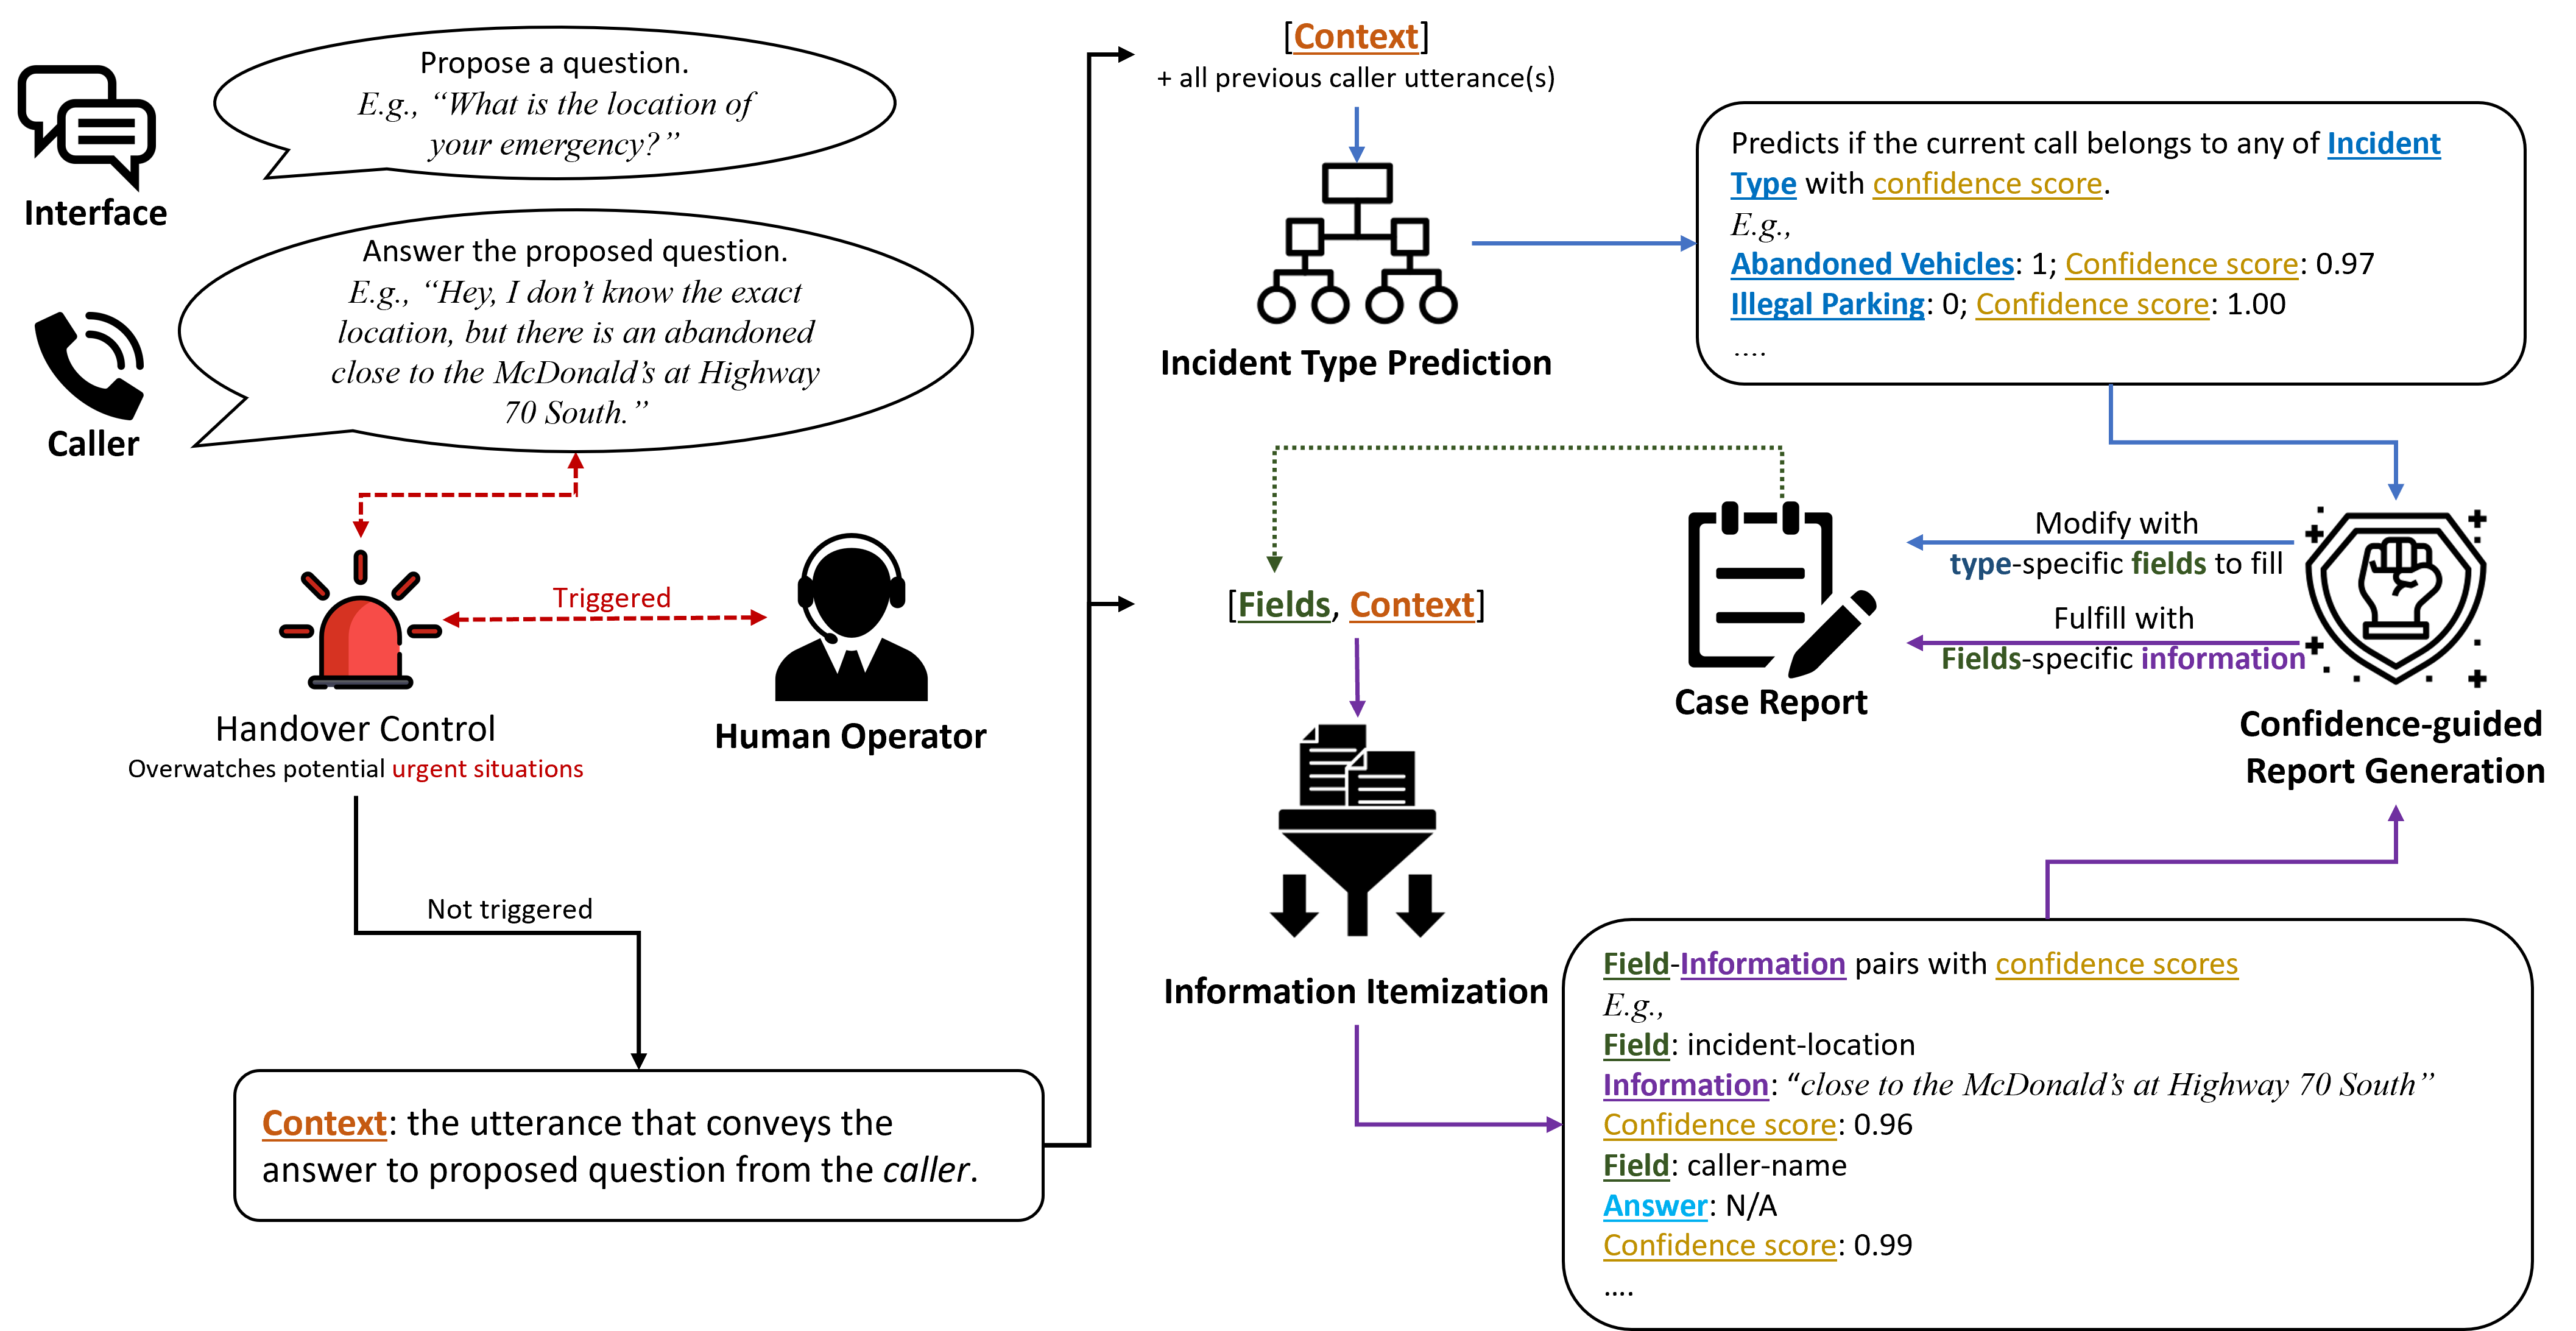
\includegraphics[width=0.9\textwidth]{figures/running_example.png}
    \caption{Running Example within One Turn of Conversation}
    \label{fig:running_example}
    \vspace{-0.5cm}
\end{figure*}

Our dataset includes real-world audio recordings covering from November 2022 to February 2023 across over 11 non-emergency types, we focus on the most common 11 incident types in this paper. Incident types are carefully annotated by dispatchers from the emergency response center.

In this section, we introduce our dataset in more detail. Initially, the dataset consists of 11,796 real recordings from the local call center. To convert the audio files in textual format for Auto311 to learn, we transcribe the audio with speaker diarization \cite{openai_whisper_2022, Bredin_pyannote_2020}. Following is one sample transcription from our dataset reporting an abandoned vehicle with private and sensitive information masked.

\noindent[00:00:13.727]--[00:00:16.458] $\mathsf{Dispatcher}$: Police Fire and Medical. 

\noindent[00:00:17.121]--[00:00:36.458] $\mathsf{Caller}$: Oh, good morning. Um, there is a car that seems to be abandoned, uh, across the street. And I just wondered if someone could check it out. It hasn't moved in weeks and weeks and weeks, and it's got kind of tinted windows and it's just creepy.

\noindent[00:00:36.863]--[00:00:38.061] $\mathsf{Dispatcher}$:  Okay, where is it located?

\noindent[00:00:39.023]--[00:01:05.483] $\mathsf{Caller}$: It is across the street from \textit{\#masked\_address}, and that's \textit{\#masked\_address}. It's in front of like a very small green space. There are kids that play in that green space, and we just all kind of, you know, creeped out about it.

\noindent[00:01:05.685]--[00:01:11.372] $\mathsf{Dispatcher}$:  Okay, so \textit{\#masked\_address}. What kind of vehicle is it?

\noindent[00:01:12.182]--[00:01:31.842] $\mathsf{Caller}$:  It is a very dark grey Volvo I believe is what it is. It's a very dark grey car and the windows are tinted just a bit.

\noindent[00:01:35.740]--[00:01:47.316] $\mathsf{Dispatcher}$: Alright, and what's your first and last name?

\noindent[00:01:48.261]--[00:01:49.746] $\mathsf{Caller}$: Okay, my name is \textit{\#masked\_personal\_information}.

\noindent[00:01:50.421]--[00:01:52.598] $\mathsf{Dispatcher}$: Did you want to speak to an officer when they come out?

\noindent[00:01:53.340]--[00:01:55.517] $\mathsf{Caller}$:  No, there's no need for that.

\noindent[00:01:55.956]--[00:02:05.204] $\mathsf{Dispatcher}$:  Alright, I will get someone out there across \textit{\#masked\_address} as soon as we can, okay?

\noindent[00:02:05.912]--[00:02:09.642] $\mathsf{Caller}$:  That sounds great. Thank you so much and I hope you have a real good day.

\noindent[00:02:09.574]--[00:02:10.013] $\mathsf{Dispatcher}$:  You too, bye.



\section{One Example Turn of Auto311}
A further example in Auto311 is also provided in Figure \ref{fig:running_example}.

\section{Handover Control Patterns}

We denote the ongoing user utterance as $\mathsf{S}$, the set of patterns as $p_0, p_1, ..., p_n \subset \mathsf{P}$, and the whole process as a boolean function $\mathsf{is\_trigger(S, {P})}$. Our rule-based procedure can be concluded using the following pseudo-logic: 

``if any pattern $p$ of $\mathsf{P}$ exists in $\mathsf{S}$, then $\mathsf{is\_trigger(S, {P})}$ returns true, the handover control is triggered, and the system interactions will be ceased and the call will be rerouted to a real operator immediately. Otherwise, $\mathsf{is\_trigger(S, {P})}$ returns false and the handover control continues over-watching the ongoing call.'' 

\begin{table}[h]
\centering
\scriptsize
\caption{Example patterns in handover control}
\begin{tabular}{||c|c|c||}
\hline
Cases                                       & Example Patterns             & Example Texts      \\ \hline\hline
\multirow{2}{*}{Request Human Operators} & {[}NP$\ast${]}                    & real human         \\ \cline{2-3} 
                                            & {[}VP$\ast${]}                    & end the call       \\ \hline
\multirow{2}{*}{Alert Potential Urgency} & {[}PRP{]}{[}be{]}{[}ADJP$\ast${]} & he is unresponsive \\ \cline{2-3} 
                                            & {[}VP$\ast${]}{[}be{]}{[}NP$\ast${]}   & guns are fired     \\ \hline
\end{tabular}
\label{tab:patterns}
\end{table}

Here we provide several patterns in Table \ref{tab:patterns}, where VP, NP, PRP, ADJP, and PP refer to verb phrases, noun phrases, personal phrases, adjective phrases, and prepositional phrases. We mark phrases that need to be maintained during runtime using sensitive keywords using stars ($\ast$). Note, this is not an exhaustive table, both patterns and sensitive keywords will be extended during usage.




\section{Phone tree of Incident Types}
We work with city authorities and create the following phone tree for different incident types, including 11 types of incidents including, illegal parking, abandoned vehicle, aggressive driver, lost-stolen, damaged property, found property, drug pros, check welfare, and noise violation. Each event has its only specific fields to fill alongside each call. The phone tree is in Figure \ref{fig:phone_tree}, we only show 9 incident types here due to the page size.


\subsection{Additional Evaluation} 

\begin{table}[]
\footnotesize
\begin{tabular}{||c|cccc||}
\hline
          & \multicolumn{4}{c||}{Illegal Parking(binary)}                                                                                                 \\ \hline\hline
Metric    & \multicolumn{1}{c|}{Precision}         & \multicolumn{1}{c|}{Recall}            & \multicolumn{1}{c|}{F-1}               & Accuracy          \\ \hline
LSTM      & \multicolumn{1}{c|}{53.85\%}           & \multicolumn{1}{c|}{87.79\%}           & \multicolumn{1}{c|}{70.00\%}           & 53.85\%           \\ \hline
CNN       & \multicolumn{1}{c|}{0.00\%}                 & \multicolumn{1}{c|}{0.00\%}                 & \multicolumn{1}{c|}{0.00\%}                 & 0.00\%                 \\ \hline
RCNN      & \multicolumn{1}{c|}{0.00\%}                 & \multicolumn{1}{c|}{0.00\%}                 & \multicolumn{1}{c|}{0.00\%}                 & 0.00\%                 \\ \hline
RNN       & \multicolumn{1}{c|}{25.00\%}           & \multicolumn{1}{c|}{28.57\%}           & \multicolumn{1}{c|}{26.67\%}           & 15.38\%           \\ \hline
Self-Attn & \multicolumn{1}{c|}{0.00\%}                 & \multicolumn{1}{c|}{0.00\%}                 & \multicolumn{1}{c|}{0.00\%}                 & 0.00\%                 \\ \hline
Attention & \multicolumn{1}{c|}{55.56\%}           & \multicolumn{1}{c|}{71.42\%}           & \multicolumn{1}{c|}{62.50\%}           & 53.85\%           \\ \hline
Bert      & \multicolumn{1}{c|}{100.00\%} & \multicolumn{1}{c|}{100.00\%} & \multicolumn{1}{c|}{100.00\%} & 100.00\% \\ \hline
\textbf{Auto311}   & \multicolumn{1}{c|}{\textbf{100.00\%}} & \multicolumn{1}{c|}{\textbf{100.00\%}} & \multicolumn{1}{c|}{\textbf{100.00\%}} & \textbf{100.00\%} \\ \hline
\end{tabular}
\label{table:rest_eval}
\caption{Auto311 on Incident Type Prediction}
\end{table}

\subsubsection{Evaluation on Incident Type Prediction}
Here we provide the rest evaluation of Auto311 on incident prediction, specifically on illegal parking and found property. The last layer of the incident type prediction module contains a binary classification of illegal parking and found property, see Table 4 for more details. As we can tell from the table, with the introduction of confidence guidance, Auto311 leverages the strong prior knowledge from BERT, yielding 100.00\% F-1 scores on both incident types.


% \section{Phone Tree to Handle Different Incident Type}



\subsubsection{Validating Proposed Metric for Text Comparison}

We conduct an evaluation to assess the effectiveness of our proposed text comparison metric, targeting the question ``How does this new text comparison work in this specific scenario?''. For this evaluation, we manually selected three distinct groups of text pairs:
\begin{itemize}
    \item \textbf{Group one} consists of text pairs that are entirely dissimilar, for instance, ``65 South exit 92'' and ``Silver Camaro.'' These pairs serve as a benchmark to evaluate how well the metric can discern vastly different information.
    \item \textbf{Group two} comprises pairs that exhibit slight differences in their content, but these discrepancies are not significant enough to significantly impact the dispatcher's decision-making process. For example, pairs like ``an SUV type truck'' and ``It's like an SUV type truck, maybe a Tahoe'' fall under this category.
    \item \textbf{Group three} contains pairs with identical or highly similar information, which are relevant for dispatchers to complete internal reports. Examples of such pairs include ``on the West End Ave'' and ``West End Ave.''
\end{itemize}

To test the consistency scores, we utilize traditional metrics like BLEU \cite{papineni2002bleu}, Damerau–Levenshtein Distance (DLD) \cite{damerau1964technique}, and ROUGE \cite{lin-2004-rouge}, in addition to our modified metric. The evaluation aims to compare how each metric performs in distinguishing differences and similarities within the text pairs across these distinct groups. This analysis will provide valuable insights into the efficacy of our proposed metric compared to established text comparison metrics.

\begin{figure}[h]
    \centering
    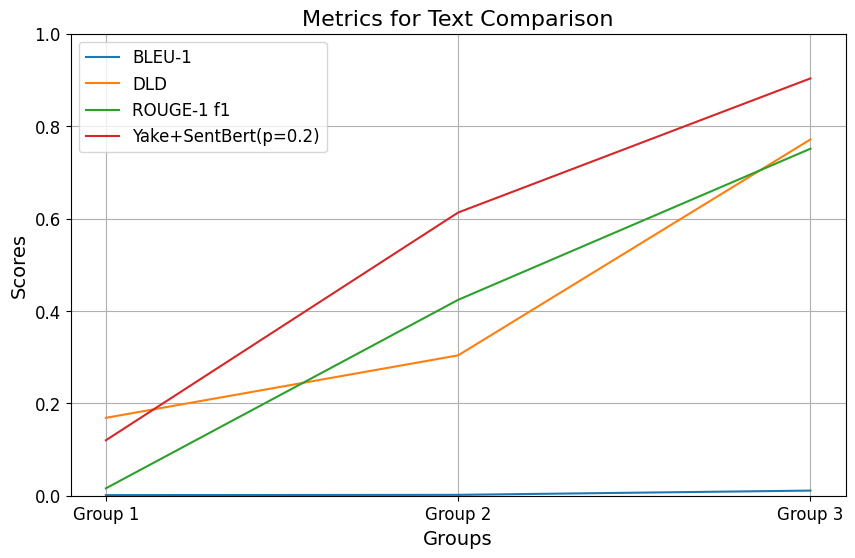
\includegraphics[width=0.40\textwidth]{figures/line-graph.png}
    \caption{Metric for Text Comparison}
    \label{fig:textcompare}
    \vspace{-0.5cm}
\end{figure}

Analysis of the plot reveals certain transitional metrics display an upward trend while failing to furnish a fair assessment. The ideal metric yields low scores for group one pair comparisons and high scores for group three pairs. As Figure \ref{fig:textcompare} displays, although exhibiting increased scores from group one to group three, DLD and ROUGE do not account for the robust correlations among text pairs in group three.

% From analyzing the plot, it is clear that some of the transitional metrics exhibit an upward trend, yet they do not provide a just assessment score. Ideally, we require a metric that yields a low score when comparing group one pairs and a high score when comparing group three pairs. The plot displays in figure \ref{fig:textcompare} reveals that DLD and ROUGE, despite their increasing scores from group 1 to group 3, fail to account for the high correlations among text pairs in group 3. 

\textit{Ultimately, from the results, it indicates our proposed text comparison metric proves more effective in assessing texts for consistency in this non-emergency dispatching scenario.}

% The objective is to demonstrate the effectiveness of the text comparison method we propose. We ask dispatchers to (1) evaluate the consistency among a list of texts in a real-world dispatching task, (2) compare our metric with their score, and (3) ask them if the scores make more sense.



\section{Discussion and Future Work}
This section discusses potential future work to enhance our proposed system based on additional findings from dataset review and development planning.

\subsubsection{Address Validation}
Location information is critical in emergency response systems. However, callers often describe locations using landmarks, not addresses. Descriptions like ``the McDonald's at Charlotte Pike'' are implicit. Translating these to explicit addresses or coordinates could better locate incidents. This work highlights address information from caller utterances without additional validation.

% Location information remains critical in an emergency and non-emergency response systems. However, callers frequently describe locations using conspicuous buildings or common spots during phone conversations. These qualitative location descriptions warrant further validation or clarification for location-sensitive tasks like emergency response. For instance, locations such as ``the McDonald's at Charlotte Pike'' or ``the Walmart entrance'' constitute implicit or ambiguous information. Hence, translating casual descriptions into explicit address details, ideally, coordinates, could better locate incidents. Presently, this work solely highlights address information from caller utterances without additional validation.

\subsubsection{Redundant Call and Callback Handling}
Redundant calls frequently occur reporting identical incidents. For instance, when witnesses spot a highway car crash, multiple people may call to report the same event, providing descriptions like ``there is a car wreck on I-440, milestone 76'' or ``there is a severe car crash on Interstate 440.'' While calling about the same incident, each call can still furnish unique unobtainable information. Similarly, caller callbacks regarding the same incident often provide previously omitted details, e.g., ``Hey, I just called a few minutes ago reporting an aggressive driver on I-40, I think the driver is in a blue Toyota, I just saw him.'' Hence, skipping or terminating ostensibly redundant calls proves inappropriate. Instead, solutions should strategically emphasize novel information despite referring to a previously reported incident. Presently, we treat each incoming call equivalently without assigning differential importance to any information we attempt to collect.


\begin{figure*}[ht]
\centering
\rotatebox{90}{
  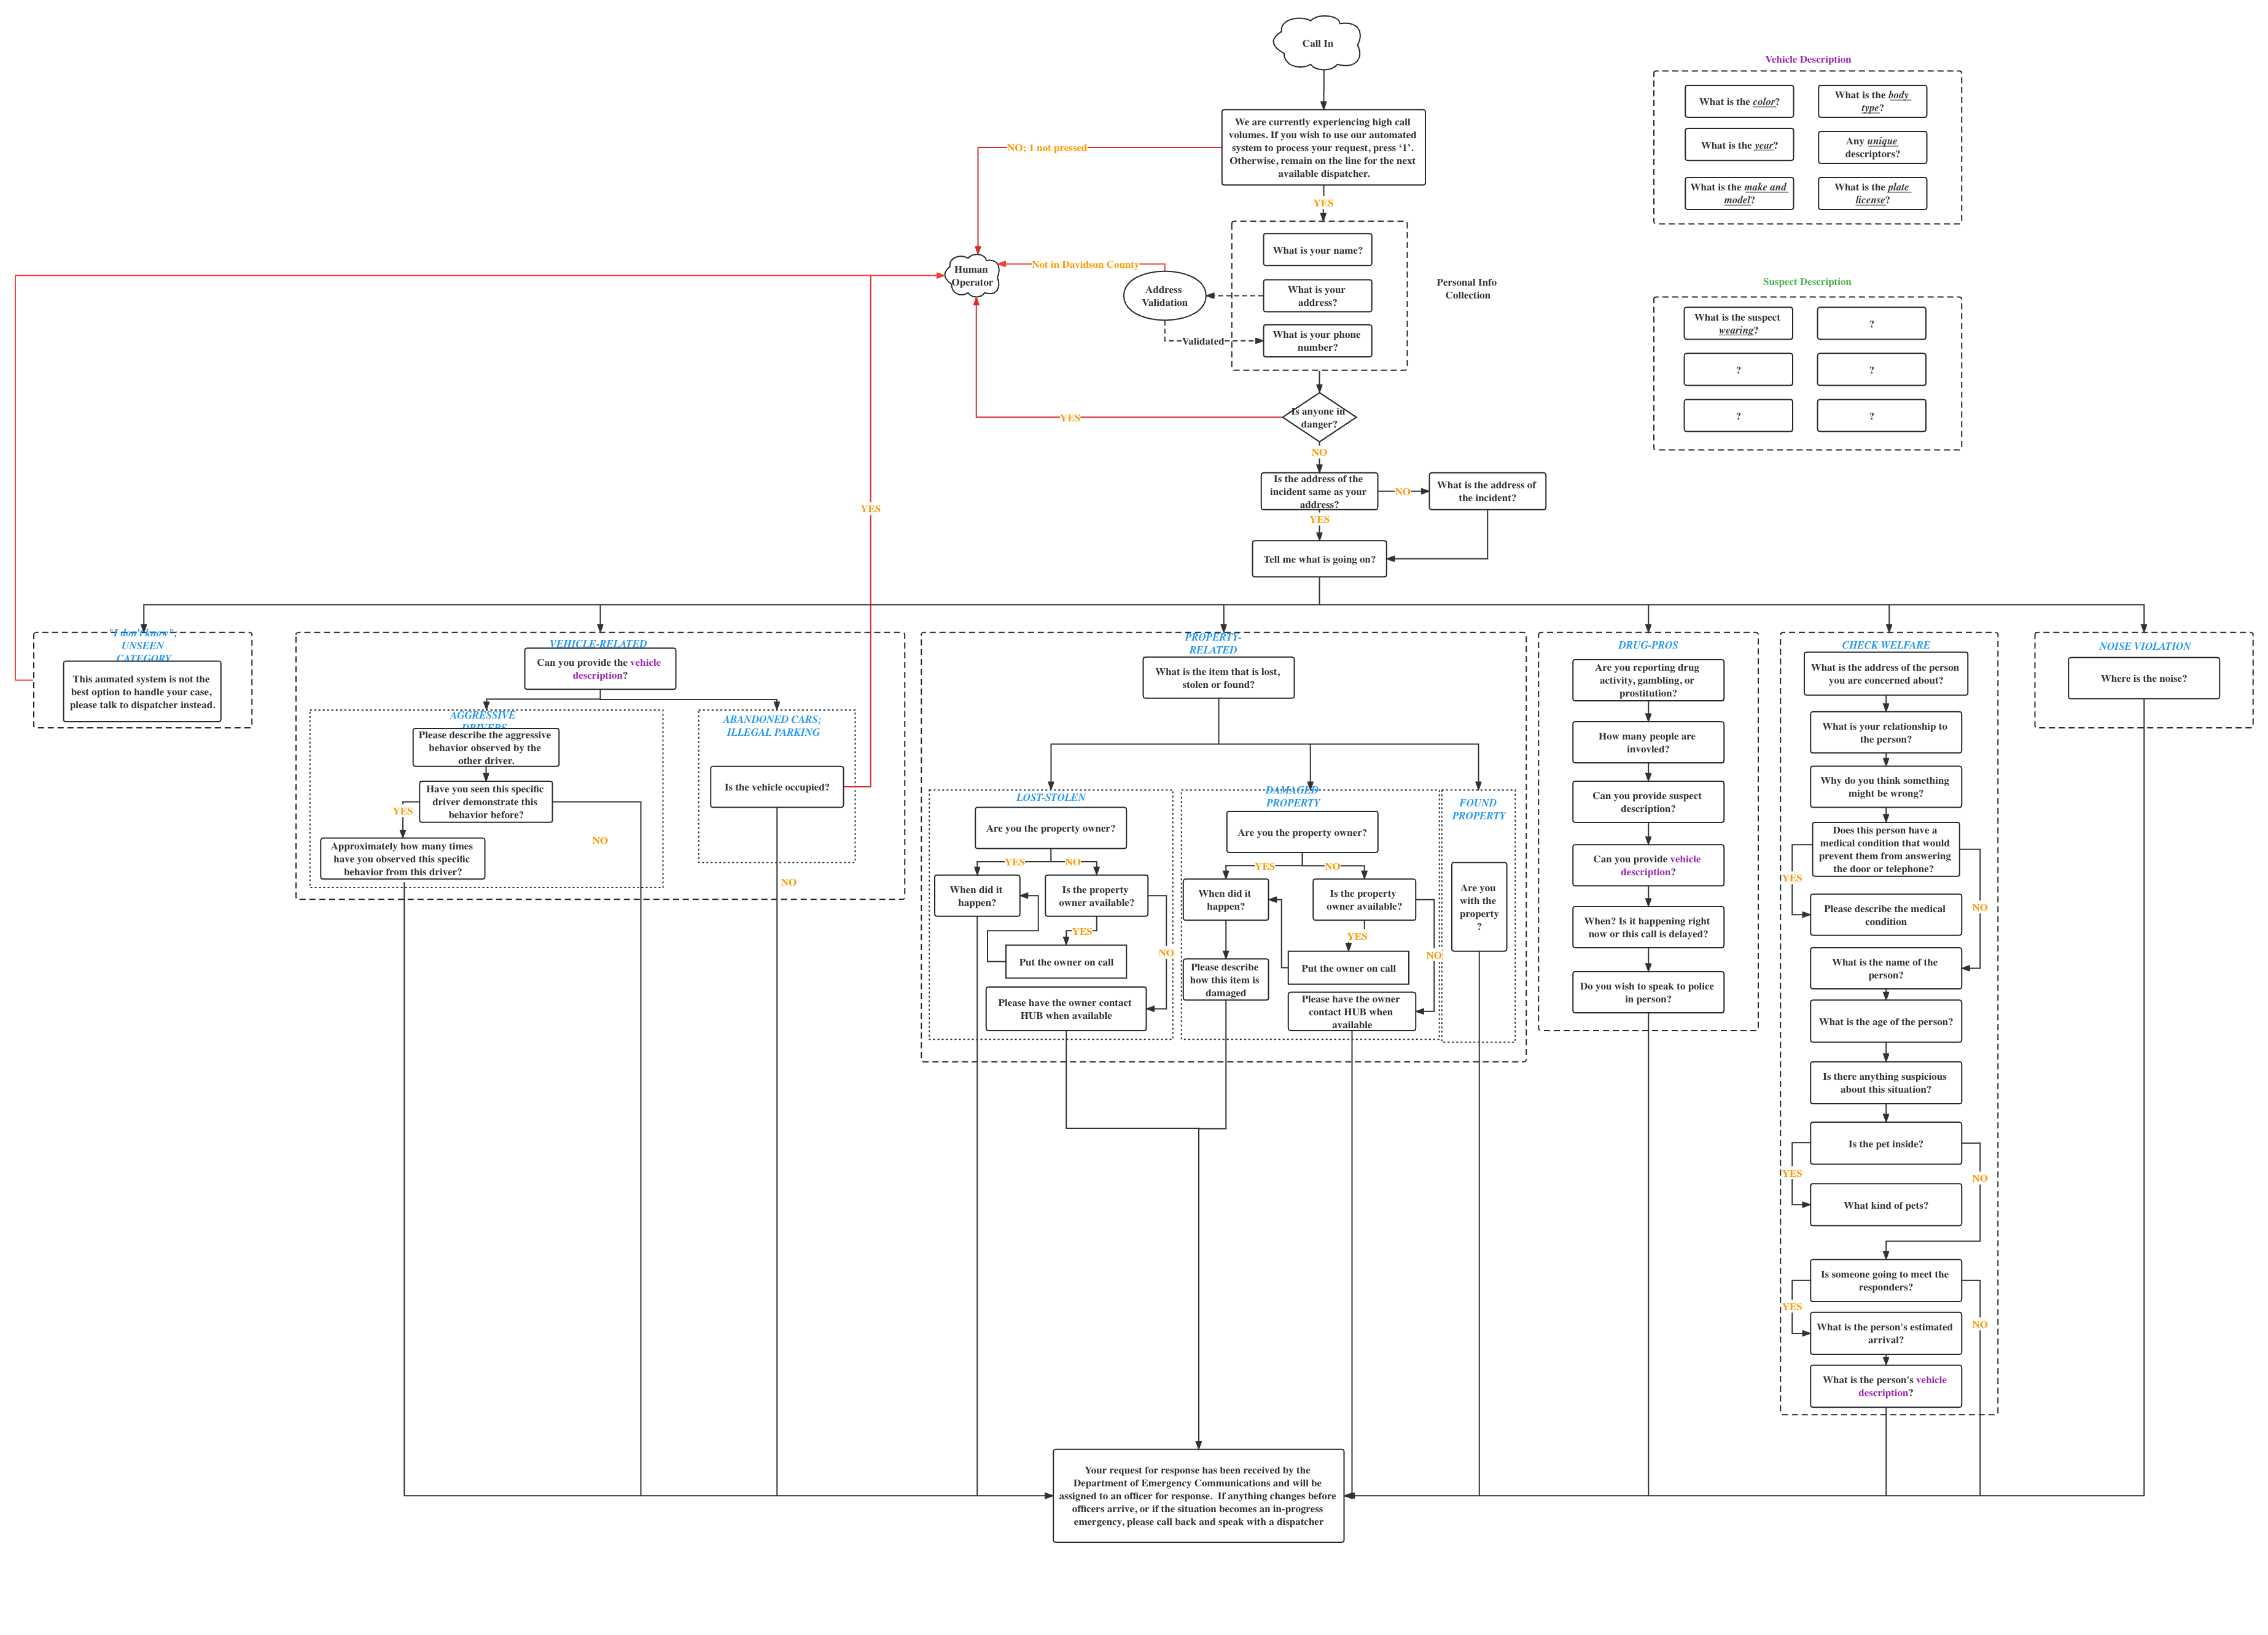
\includegraphics[width=1.4\textwidth]{figures/CIVIC-311.png} 
}
\caption{Phone Tree for Incident Handling} 
\label{fig:phone_tree}
\end{figure*}

\begin{table}[]
\footnotesize
\begin{tabular}{||c|c|c|c|c||}
\hline
          & Minor Crash Report & Lost-Stolen & Aggressive Drivers & Damaged Property \\ \hline\hline
LSTM      & 56.47\%            & 0.00\%      & 53.85\%            & 0.00\%           \\ \hline
CNN       & 75.86\%            & 85.71\%     & 72.72\%            & 40.00\%          \\ \hline
RCNN      & 90.57\%            & 82.35\%     & 61.54\%            & 76.92\%          \\ \hline
RNN       & 63.33\%            & 40.00\%     & 52.71\%            & 44.44\%          \\ \hline
Self-Attn & 88.46\%            & 88.89\%     & 66.67\%            & 66.67\%          \\ \hline
Attention & 91.69\%            & 62.50\%     & 50.00\%            & 54.55\%          \\ \hline
Bert      & 95.04\%            & 95.60\%     & 92.31\%            & 88.89\%          \\ \hline
\textbf{Auto311}   & \textbf{95.71\%}            & \textbf{96.70\%}     & \textbf{93.75\%}            & \textbf{94.12\%}          \\ \hline
\end{tabular}
\end{table}
\end{document}
